\section{Měření polohy - principy odporové, indukčnostní, kapacitní}
\subsection{Odporové snímače polohy}

\subsubsection{Snímače se skokovou změnou odporu}
Mechanicky ovládané kontakty:
\begin{itemize}
    \item Mechanické mikrospínače - ovládání světla
    \item Parametry: Rozsahy síly potřebné pro spínání, velikost proudu/napětí které mohou spínat(větší problém s DC proudy), životnost z pohledu počtu spínání(rychlost mechanické únavy, klasicky \(10^6\) sepnutí)
\end{itemize}
Magneticky ovládané kontakty:
\begin{itemize}
    \item Jazýčková relé - kontakty z magneticky měkkého materiálu ovládané polem permamentního magnetu
    \item Princip - k relé přibližujeme magnet, přiblížením vzniká přitažlivá síla mezi kontakty relé
    \item Parametry - spínané proudy(jednotky mA), max počet přepnutí
    \item Kontakty se mohou slepit kvůli přiliš silné magnetizaci
    \item Měření rychlosti na kole, otevření zavření dveří, atd...
\end{itemize}
\begin{figure}[h!]
    \centering
    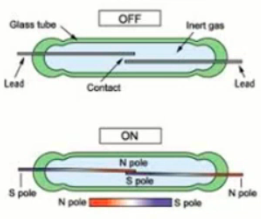
\includegraphics[scale = 0.5]{img/JazRele.png}
\end{figure}
\subsubsection{Snímače s plynulou změnou odporu}
Odporové potenciometry s pohyblivým kontaktem mechanicky spojeným s měřenou veličinou.\\
Na nevodivé podložce je nanesena vodivá vrstva, přes kterou přejíždí pohyblivý kontakt a měříme odpor mezi jezdcem a jedním z okraju vodivé dráhy.\\
Dělení podle typu jezdce:
\begin{itemize}
    \item Rotační jezdec - měření úhlového posunutí
    \item Přímočarý jezdec - měření polohy nebo lineárního posunutí
    \item Spirálový jezdec - helipot typicky s 10 závity, rozsah větší jak 360°
\end{itemize}
Lankem ovládané potenciometry, mají rozsah až 40m, rychlost 2m/s.
\begin{figure}[h!]
    \centering
    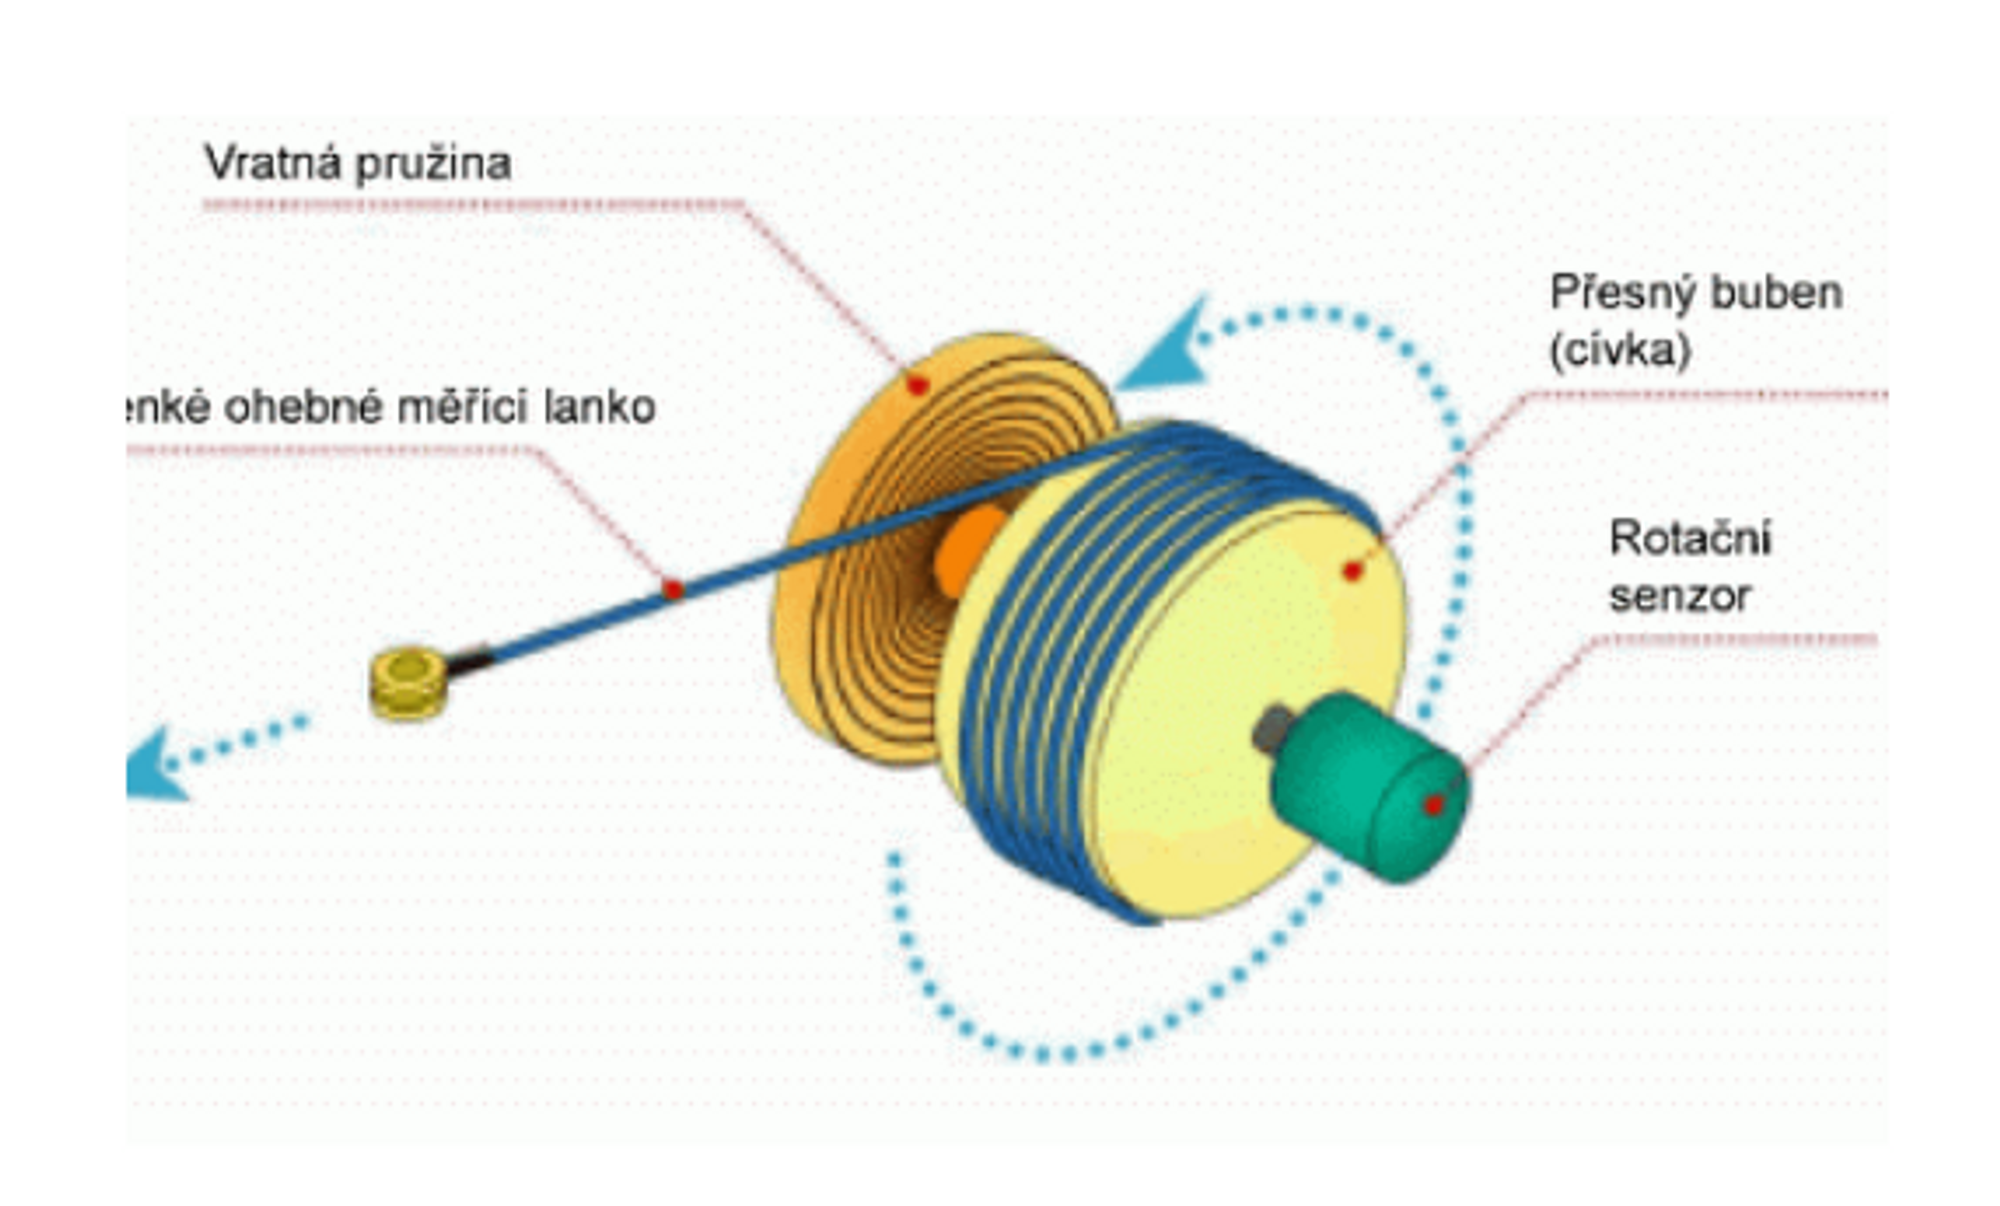
\includegraphics[scale = 0.1]{img/Lanko.png}
\end{figure}

\subsubsection{Zapojení odporových snímačů}
\begin{figure}[h!]
    \centering
    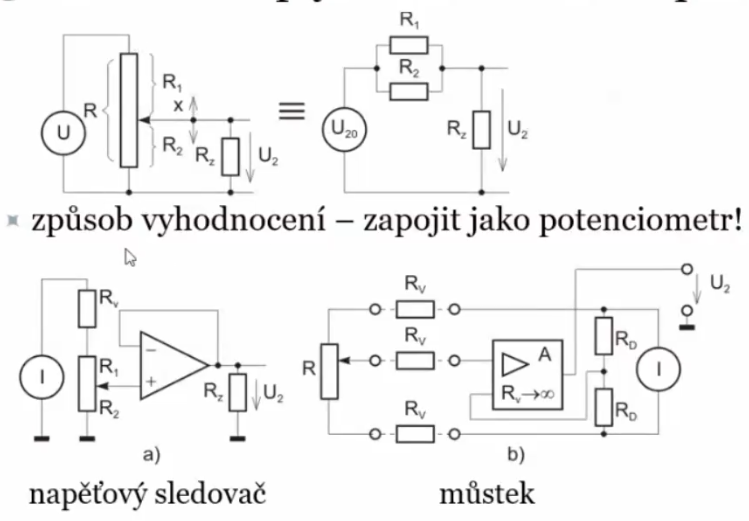
\includegraphics[scale = 0.4]{img/ZapojOdp.png}
\end{figure}
V prvním zapojení je \textit{R} samotný snímač, který se připojí na ke zdroji U, tím se stanoví rozsah a potom posouváním, které je zobrazeno proměnnou x měníme odpor. Měříme výstupní napětí \(U_2\)\\
Požadavek, aby výstupní dělič byl nezatížený, chceme aby vstupní odpor voltmetru byl poměrně veliký.\\
Je nutno zajistit aby odběr proudu z děliče byl co nejmenší, jinak se bude chovat nelineárně. To se dá řešit buď vysokým vstupním odporem voltmetru anebo napěťovým sledovačem. Pokud má voltmetr odpor větší jak 1:100 vůči měřicí kartě už nám na tomto nezáleží.\\
V zapojení napěťového sledovače je mezi zátěžový odpor a snímač zaveden napěťový zesilovač s jednotkovým zesílením. Ideální zesilovač má nekonečný vstupní a nulový výstupní odpor, což vede k tomu, že na zátěžovém odporu nezáleží.\\
Můstek, pokud máme dlouhé vodiče od snímače kde se začne projevovat odpor vodičů, výhodou je že potlačuje odpor vodičů \(R_v\).
\subsubsection{Výhody}
\begin{itemize}
    \item jednoduché zpracování signálu
    \item jednoduchá výroba, levné
    \item reprodukovatelnost, linearita
    \item odolnost proti vibracím - ne tak uplně, jen běžné průmyslové vibrace tlumí
\end{itemize}
\subsubsection{Nevýhody}
\begin{itemize}
    \item kontaktní princip
    \item šum
    \item životnost
    \item dynamické vlastnosti - kvůli mechanickým vlastnostem, měřitelná pouze pomalá změna
    \item omezený ztrátový výkon(vnitřní odpor děliče musí být menší než vstupní odpor aby nedocházelo k přehřívání)
\end{itemize}

\subsection{Indukčnostní snímače polohy}
Pasivní snímače, měřená veličina je převáděna na změnu indukčnosti(jedna nebo dvě cívky) nebo vzájemné indukčnosti(dvě nebo tři cívky).\\
Dělení indukčnostních snímačů:
\begin{itemize}
    \item Dle magnetického obvodu:
          \begin{itemize}
              \item S otevřeným magnetickým obvodem - magnetický tok prochází z velké části vzduchem
              \item S uzavřeným magnetickým obvodem - magnetický tok prochází z velké části přes magneticky vodivý materiál
          \end{itemize}
    \item Dle uspořádání cívek:
          \begin{itemize}
              \item Jednoduchá(parametrický) snímač - změna indukčnosti 1 cívky, závislost nelineární
              \item Diferenční snímač - vyhodnocujeme rozdíl dvou cívek
              \item Transformátorový snímač - 1 cívka napájecí, měříme změnu vzájemné indukčnosti napájecí s dvuma cívkama sekundárníma
          \end{itemize}
    \item Dle principu:
          \begin{itemize}
              \item Změna indukčnosti
              \item Změna vzájemné indukčnosti - LVDT, oscilátorové
          \end{itemize}
\end{itemize}

\subsubsection{Impedance cívky snímače}
\begin{center}
    \(Z(j\omega) = R + j\omega\frac{N^2}{Z_m} = R +j\omega\frac{N^2}{R_m+jX_m} = (R+ \frac{N^2\omega X_m}{\left\lvert Z_m(j\omega)\right\rvert^2 }) + j(\frac{N^2\omega R_m}{\left\lvert Z_m(j\omega) \right\rvert^2})\)
\end{center}
Kde:
\begin{itemize}
    \item R je ohmický odpor vinutí
    \item \(R_m\) a \(X_m\) jsou činná a jalová složka magnetické reluktance \(Z_m\). \(X_m = \frac{P_0}{\omega \Phi^2}\) odpovídá ztrátám vířivými proudy a hysterzí. U snímačů s vnesenou impedancí, snímačů s vířivými proudy, snímačů s potlačeným polem. \(R_m = \sum \frac{l_i}{\mu_i S_i}\) odpovídá geometrii uzavřeného magnetického obvodu. snímače s proměnnou délkou střední siločáry \(l_i\), snímače s proměnnou plochou \(S_i\) vzduchové mezery, snímače s proměnnou permeabilitou \(\mu_i\).
\end{itemize}
\begin{center}
    \(L \approx \frac{N^2}{R_m}\)
\end{center}
\subsubsection{Indukčnostní snímač s uzavřeným magnetickým obvodem}
\subsubsection*{Indukčnostní snímač s proměnnou vzduchovou mezerou}
Jednoduchý parametrický snímač s proměnnou délkou střední siločáry ve vzduchové mezeře.\\
U \(R_m\) můžeme vypustit "kovovou" část, protože děláme permeabilitou železa, která je cca 300k a tím pádem je ten zlomek zanedbatelný oproti vzduchové části.\\
Nezávislý na parazitních vlivech.\\
\newpage
\begin{figure}[h!]
    \centering
    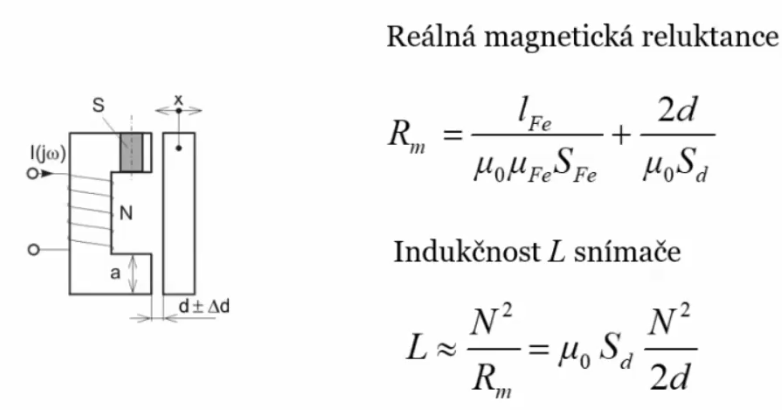
\includegraphics[scale = 0.3]{img/IndukcSPromMez.png}
\end{figure}

Diferenční snímač, přidáme stejný systém na druhou stranu (symetricky). Poté budem porovnávat rozdíl indukčností obou částí.\\
Při pohybu větší indukčnost bude na straně bude vzduchová mezera (d) menší.\\
Velmi jednoduchý,stabilní, robustní a má velkou citlivost(až extrémní).\\
Změna indučknosti napravo oproti te nalevo - můstkové zapojení. Musíme měřit nejen absolutní hodnotu napětí, ale musíme měřit i fázi výstupního signálu vůči vstupnímu signálu. Absolutní hodnotou měříme posun a fází směr posunu\
\begin{figure}[h!]
    \centering
    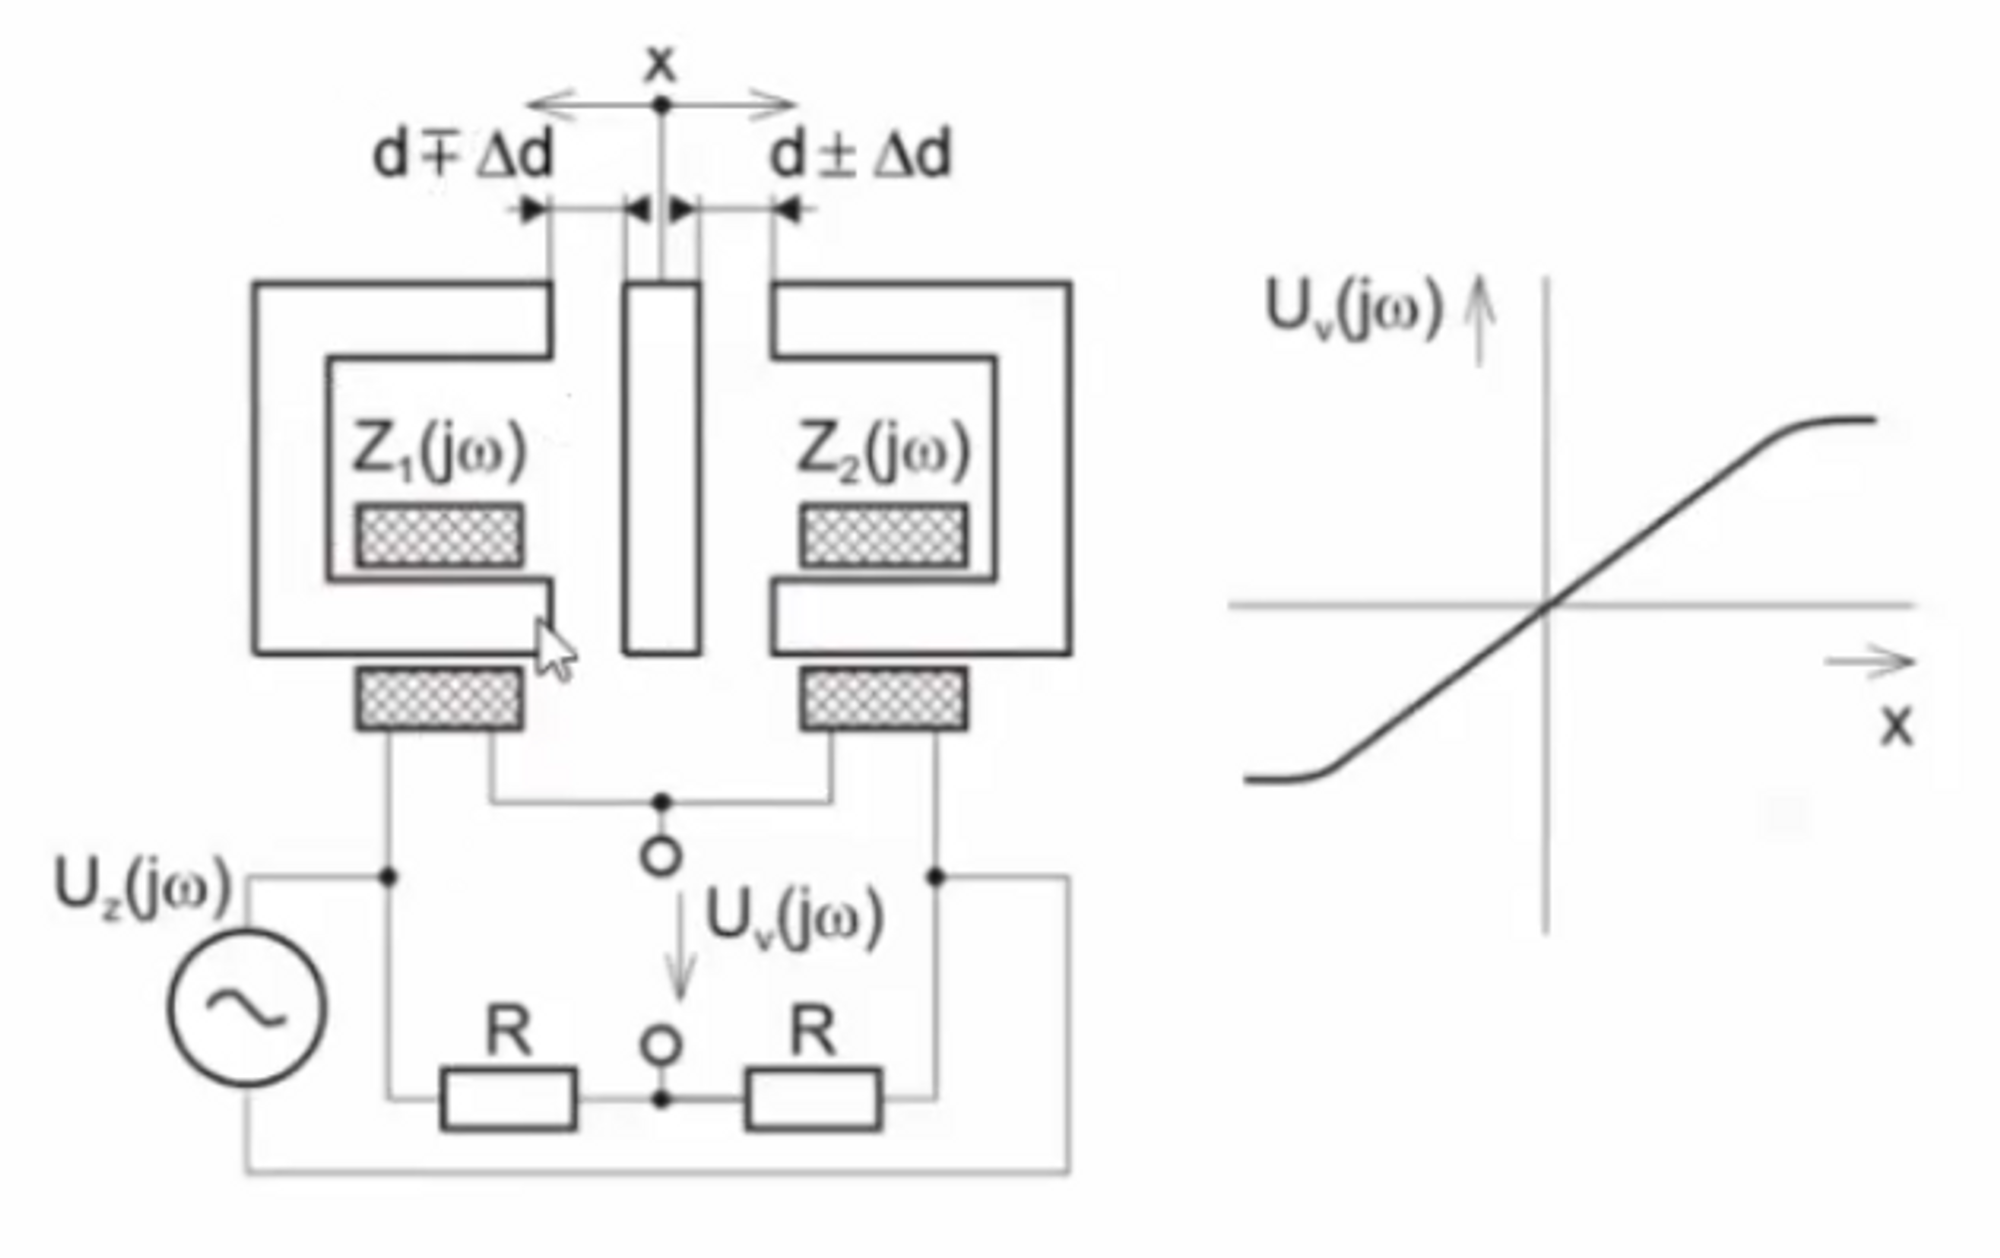
\includegraphics[scale = 0.1]{img/IndukDif.png}
\end{figure}

\subsubsection{Indukčnostní snímač s otevřeným magnetickým obvodem}
\subsubsection*{Diferenční}
Když do cívky budeme vkládat magneticky vodivý materiál, ovlivňujeme magnetickou vodivost celého obvodu a tím se mění indukčnost.\\
Snižujeme magnetický odpor a tím roste indukčnost.\\

\begin{figure}[h!]
    \centering
    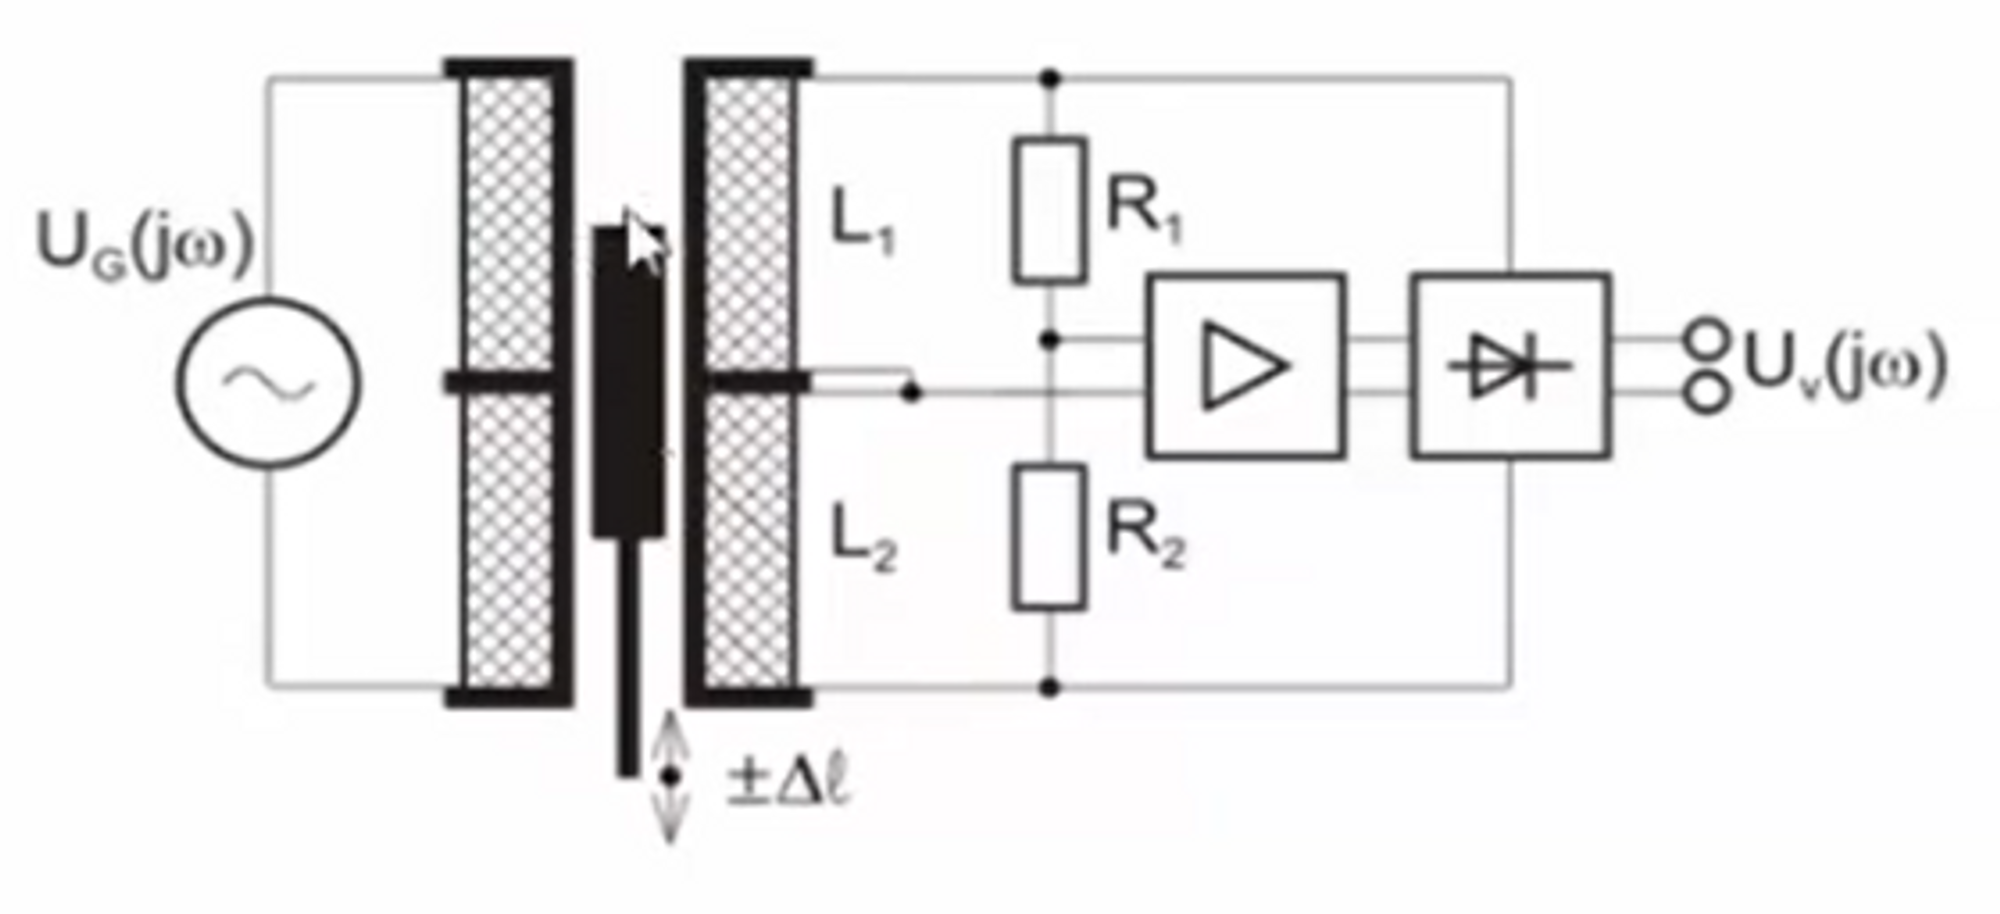
\includegraphics[scale = 0.1]{img/DifOtInd.png}
\end{figure}

Můstkové zapojení, pokud bude materiál přesně uprostřed, indukčnost cívek bude stejná, pohybem materiálu měníme indukčnosti cívek a měříme rozvážení můstku. Dioda(fázový detektor) dělá fázové vyhodnocení.\\


\subsubsection*{Transformátorový - LVDT}
LVDT - Linear variable differential transformer.\\
Častěji používaný.\\
Mění se vzájemná indukčnost mezi prostřední cívkou a cívkami na okraji.\\
Změnou polohy jádra ovlivňujeme vzájemnou indukčnost primární cívky vůči sekundárním cívkám. Pokud je materiál přesně uprostřed, pak je vzájemná indukčnost stejná vůči horní i spodní cívce. Pokud pohneme jádrem nahoru, tak větší část MP primární cívky bude procházet cívkou \(S_1\), tím se do cívky \(S_1\) bude indukovat větší napětí. Změnu vzájemné indukčnosti vyhodnocujeme měřením velikosti indukovaného napětí na sekundárních cívkách, jejich poměrem pak určujeme polohu jádra. Alternativou je vyhodnocování fáze mezi primárním a sekundárním napětím.\\

\begin{figure}[h!]
    \centering
    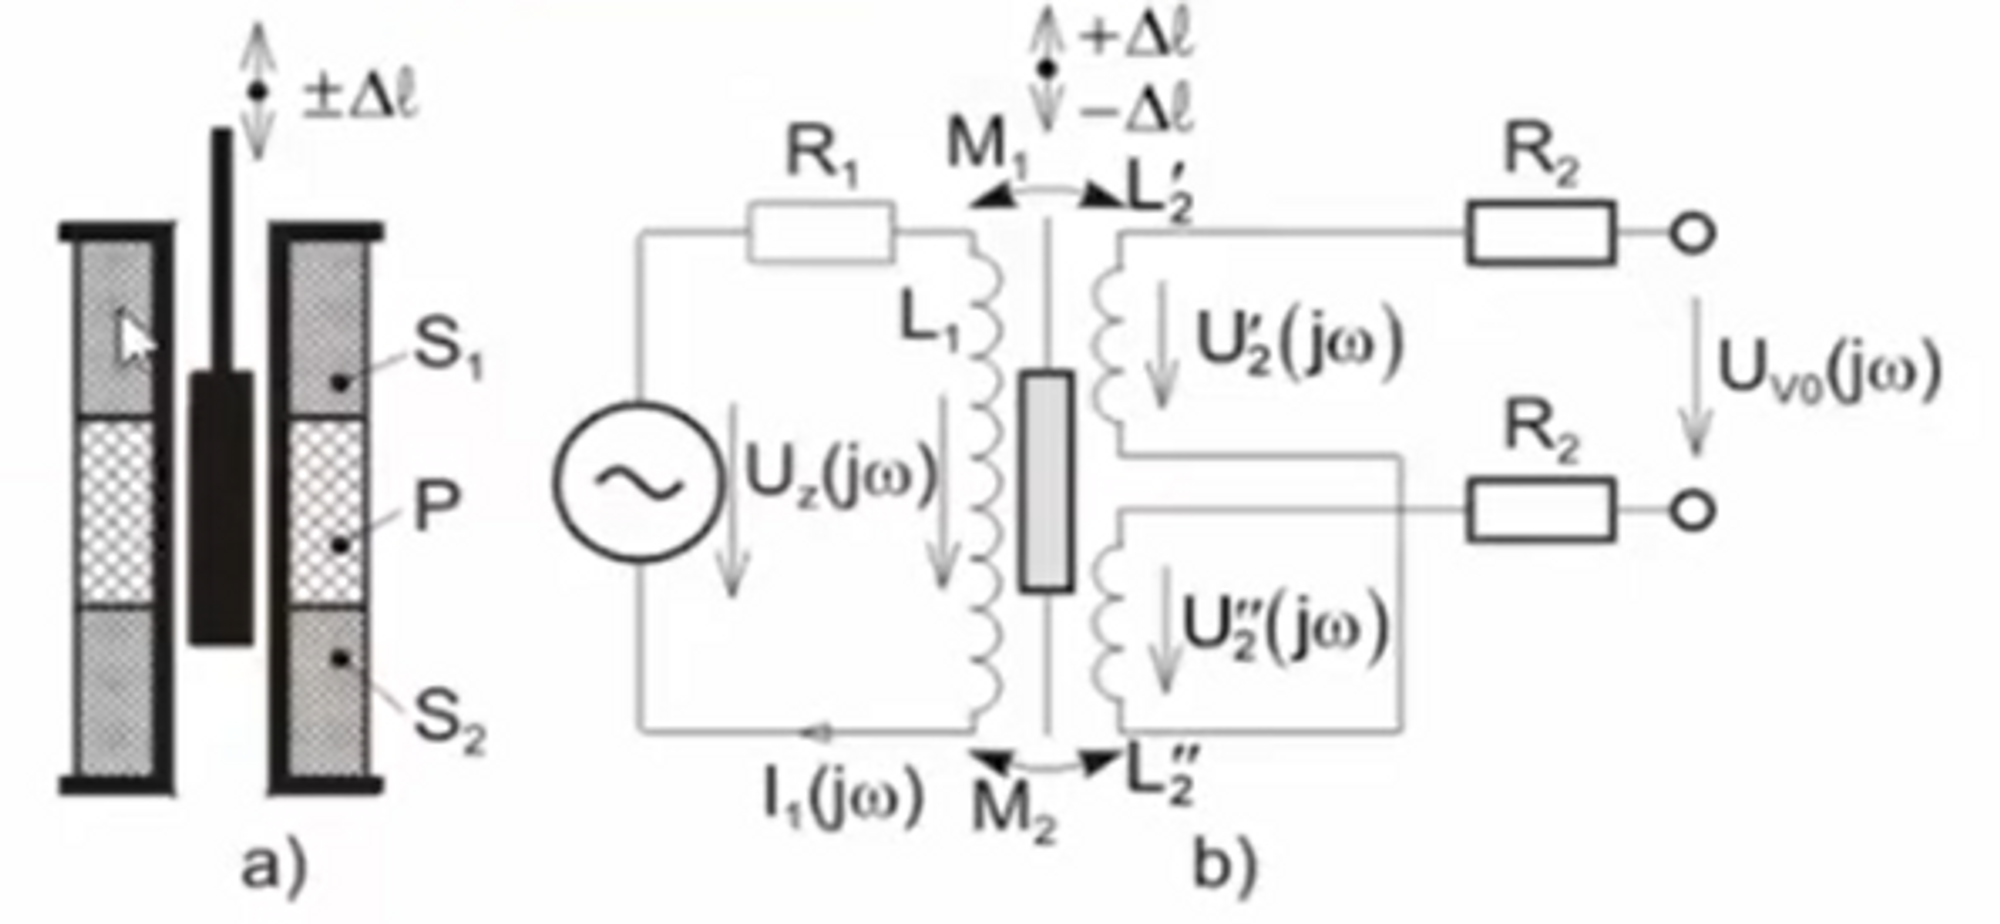
\includegraphics[scale = 0.1]{img/TransOtevInd.png}
\end{figure}

\subsubsection{Indukčnostní snímače s vířivými proudy(Eddy-current sensors)}
Také nazývány s potlačeným pólem či s vnesenou impedancí.\\
Bezkontaktní, všechny předchozí byly kontaktní.\\
Provedení s 1, 2 či 3 cívkami.\\
Snímač vzdálenosti nebo vodivosti.\\
Mějme cívku napájenou ze zdroje, taková cívka si vytvoří MP, když do něj vložíme elektricky vodivý předmět, tak v něm vzniknou vířivé proudy. Které část pole odčerpávají a přetvoří ho na teplo. Odčerpáním pole klesne indučnost cívky, což vede ke zvýšení proudu tekoucího cívkou.\\
Pokud vkládáme magneticky vodivý, ale elektricky nevodivý předmět, tak se zvyšuje indukčnost, kvůli tomu, že měníme geometrii magnetického obvodu.\\
Pokud je materiál vodivý jak elektricky tak magneticky, pak záleží na jakém kmitočtu pracujeme. Při nižších kmitočtech převažuje magnetická složka, na vysokých převažuje elektrická složka.\\
\begin{figure}[h!]
    \centering
    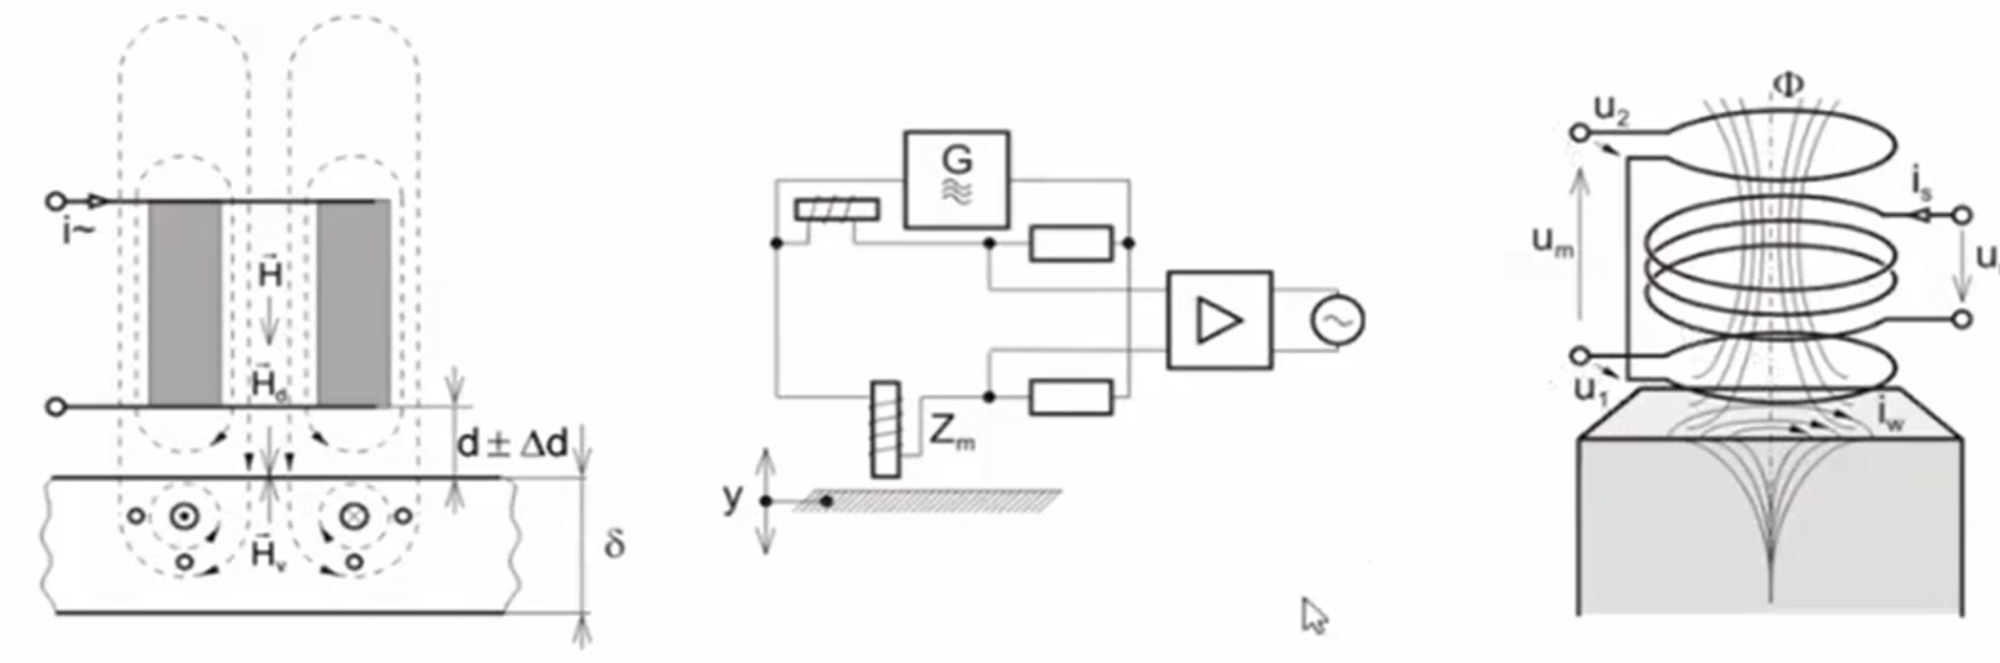
\includegraphics[scale = 0.2]{img/EddyCurr.png}
\end{figure}
Zapojení diferenční nebo transformátorové:
\begin{itemize}
    \item Diferenční - máme 2 cívky, jednu měřící a druhou referenční, měříme rozvážení můstku. Prostřední obrázek.
    \item Transformátorové - primární a 2 sekundární cívky, měříme změnu napětí na sekundárních cívkách.
\end{itemize}
Typické využití jsou binární proximitní snímače, které detekují přítomnost elekticky vodivých předmětů před aktivní plochou snímače.\\

\subsubsection{Resolver}
Snímač úhlového natočení.\\
Využití pro měření polohy hřídele motoru. Vzájemná poloha rotoru a statoru. Když bude rotor ve svislé poloze tak bude největší indukčnost sekundární cívky(\(u_2\)).\\
\begin{figure}[h!]
    \centering
    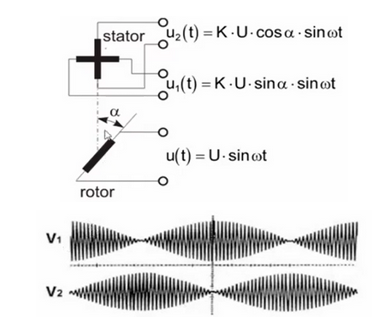
\includegraphics[scale = 0.5]{img/Resolver.png}
\end{figure}
Relativně přesný, je nahrazován optickými.\\

\subsection{Kapacitní snímače polohy}
Základní vztah:
\begin{center}
    \(C = \varepsilon \frac{S}{d} = \varepsilon_r \cdot \varepsilon_0 \frac{S}{d}\)
\end{center}
kde \(\varepsilon\) je permitivita, \(S\) je plocha elektrod a \(d\) je vzdálenost elektrod.\\
\begin{figure}[h!]
    \centering
    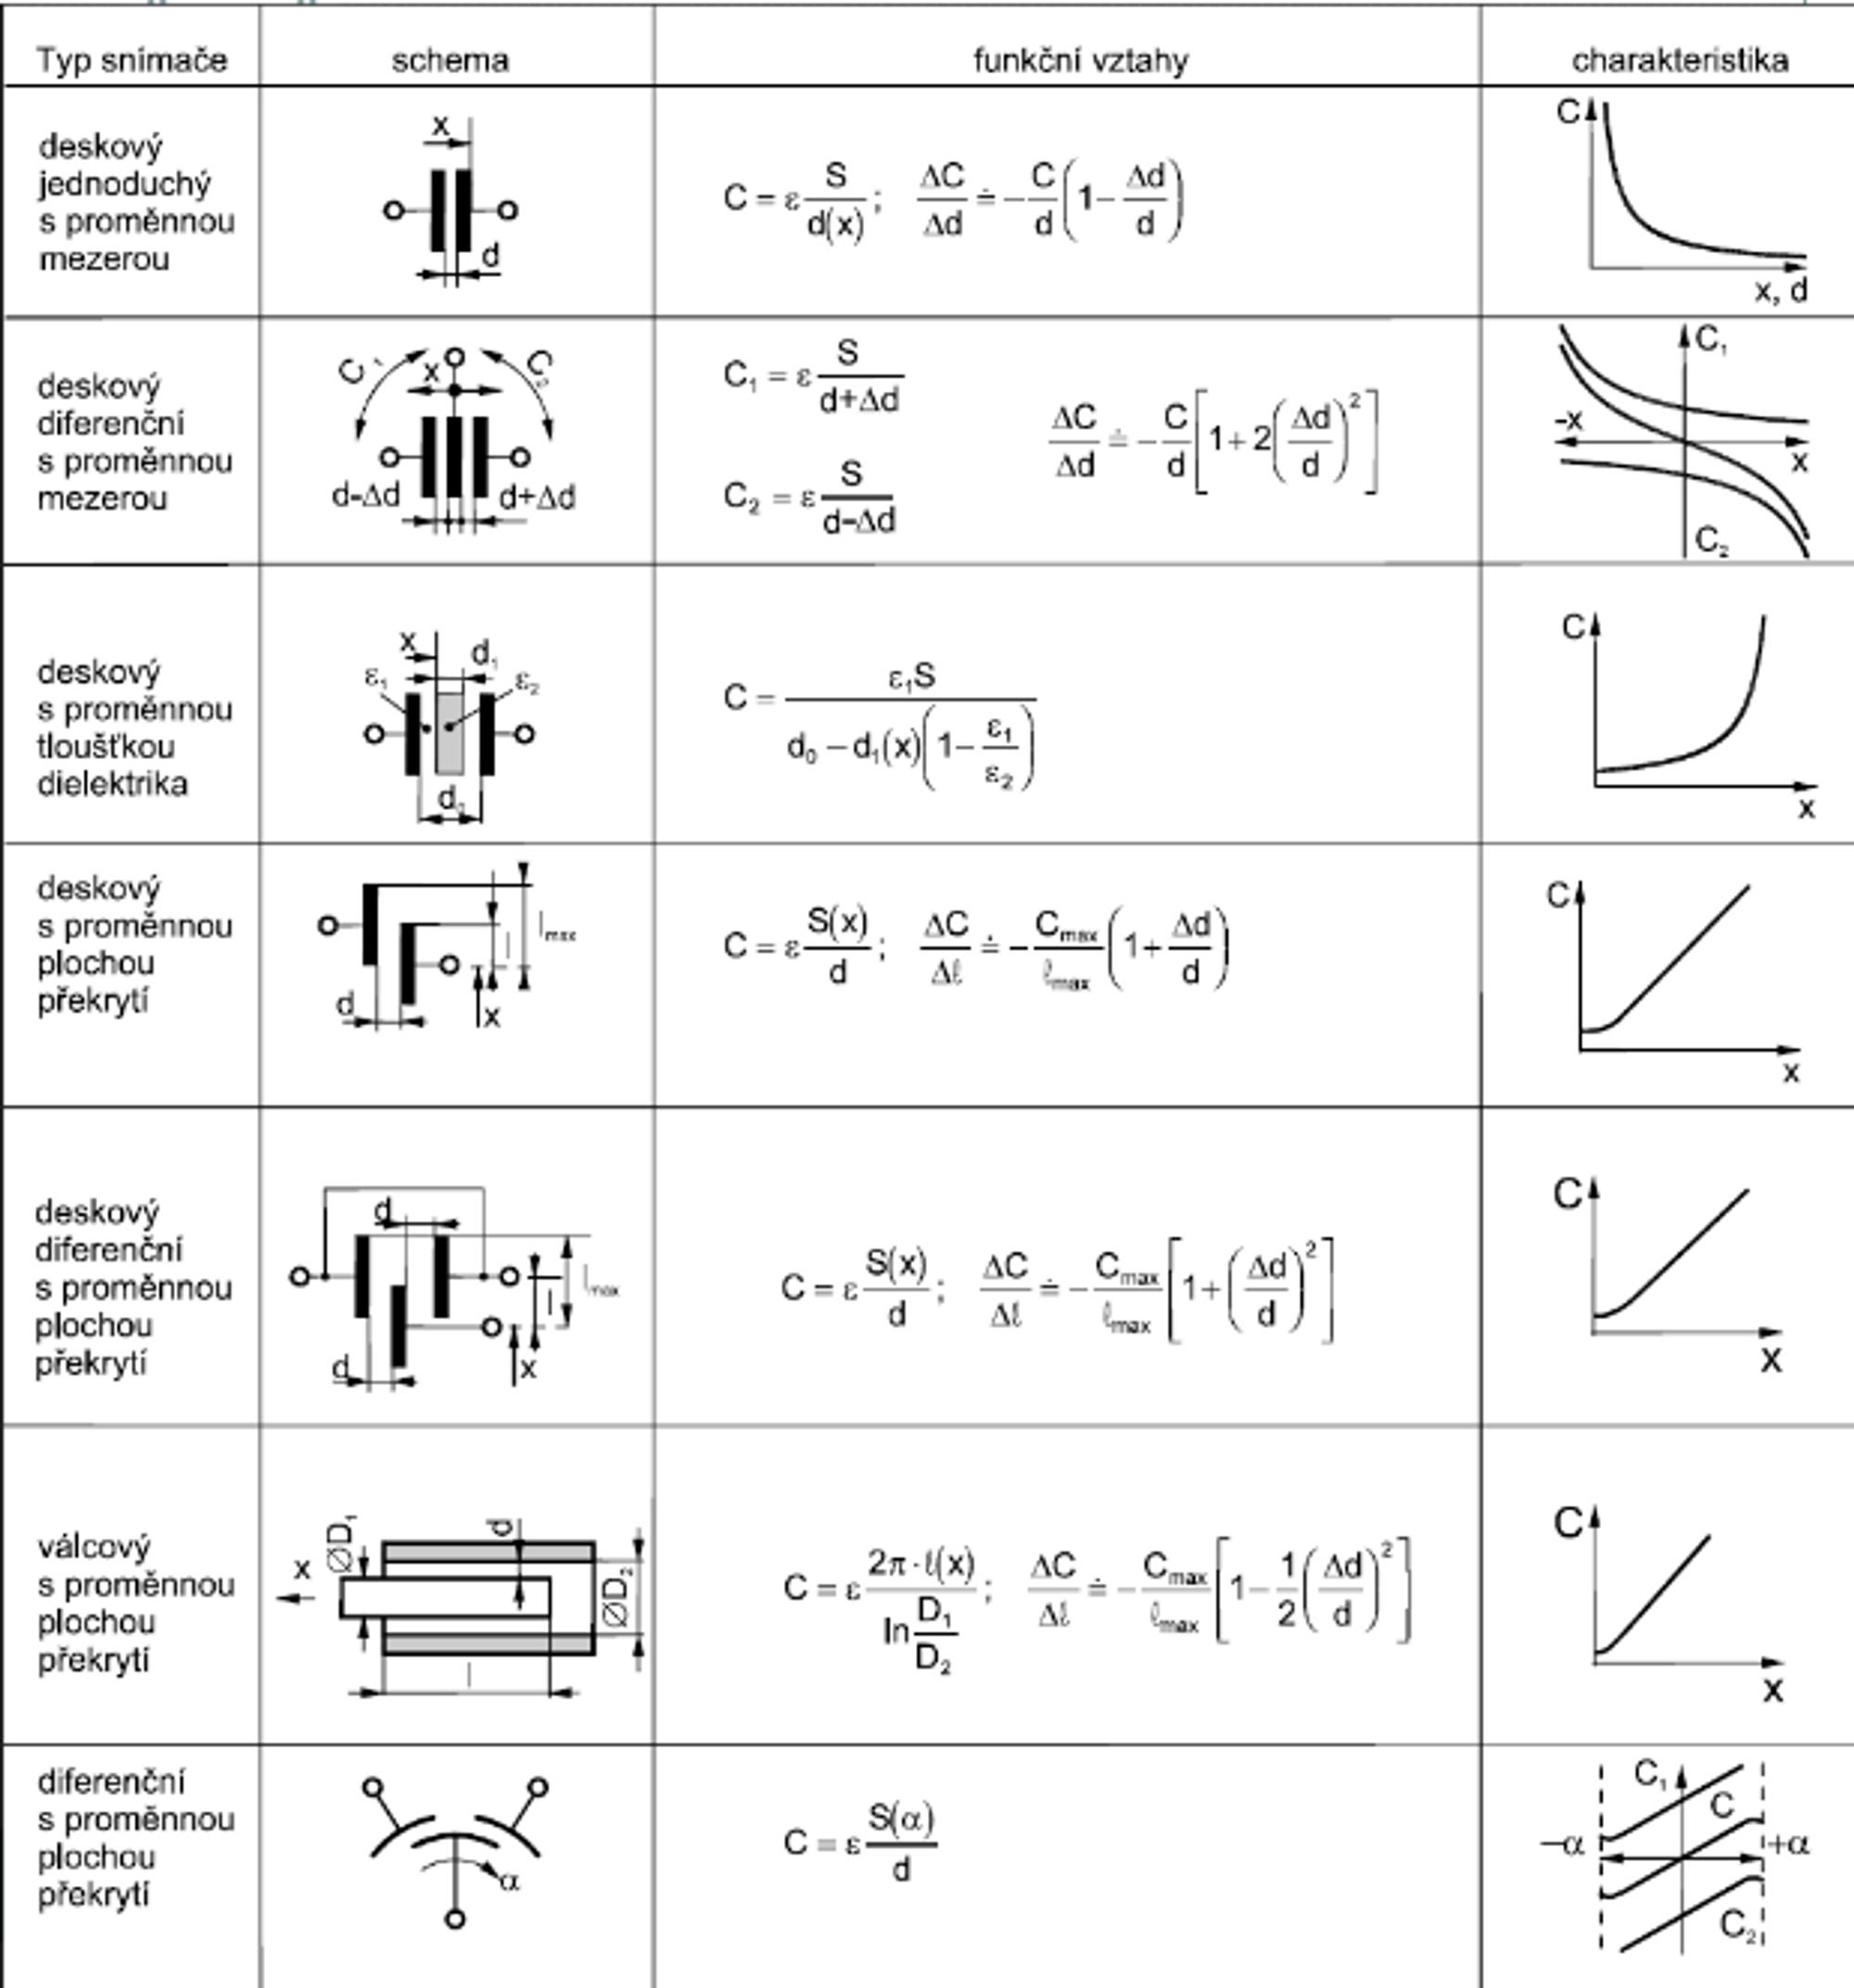
\includegraphics[scale = 0.1]{img/KapTypy.png}
\end{figure}
\subsubsection{Kapacitní senzor s proměnnou plochou překrytí}
\(C = \varepsilon \frac{S}{d}\).\\
Elektrody 1,2 pevné a elektroda 3 se pohybuje, vyhodnocujeme rozdíl.
\begin{center}
    Příklad vyhodnocení: \(\frac{C_{23}-C_{13}}{C_{23}+C_{13}}\)
\end{center}
Vzájemný poměr nezáleží ani na vzdálenosti, ani na permitivitě, tím potlačujeme téměř všechny parazitní vlivy, které nám zásadně ovlivňují měření.\\
\begin{figure}[h!]
    \centering
    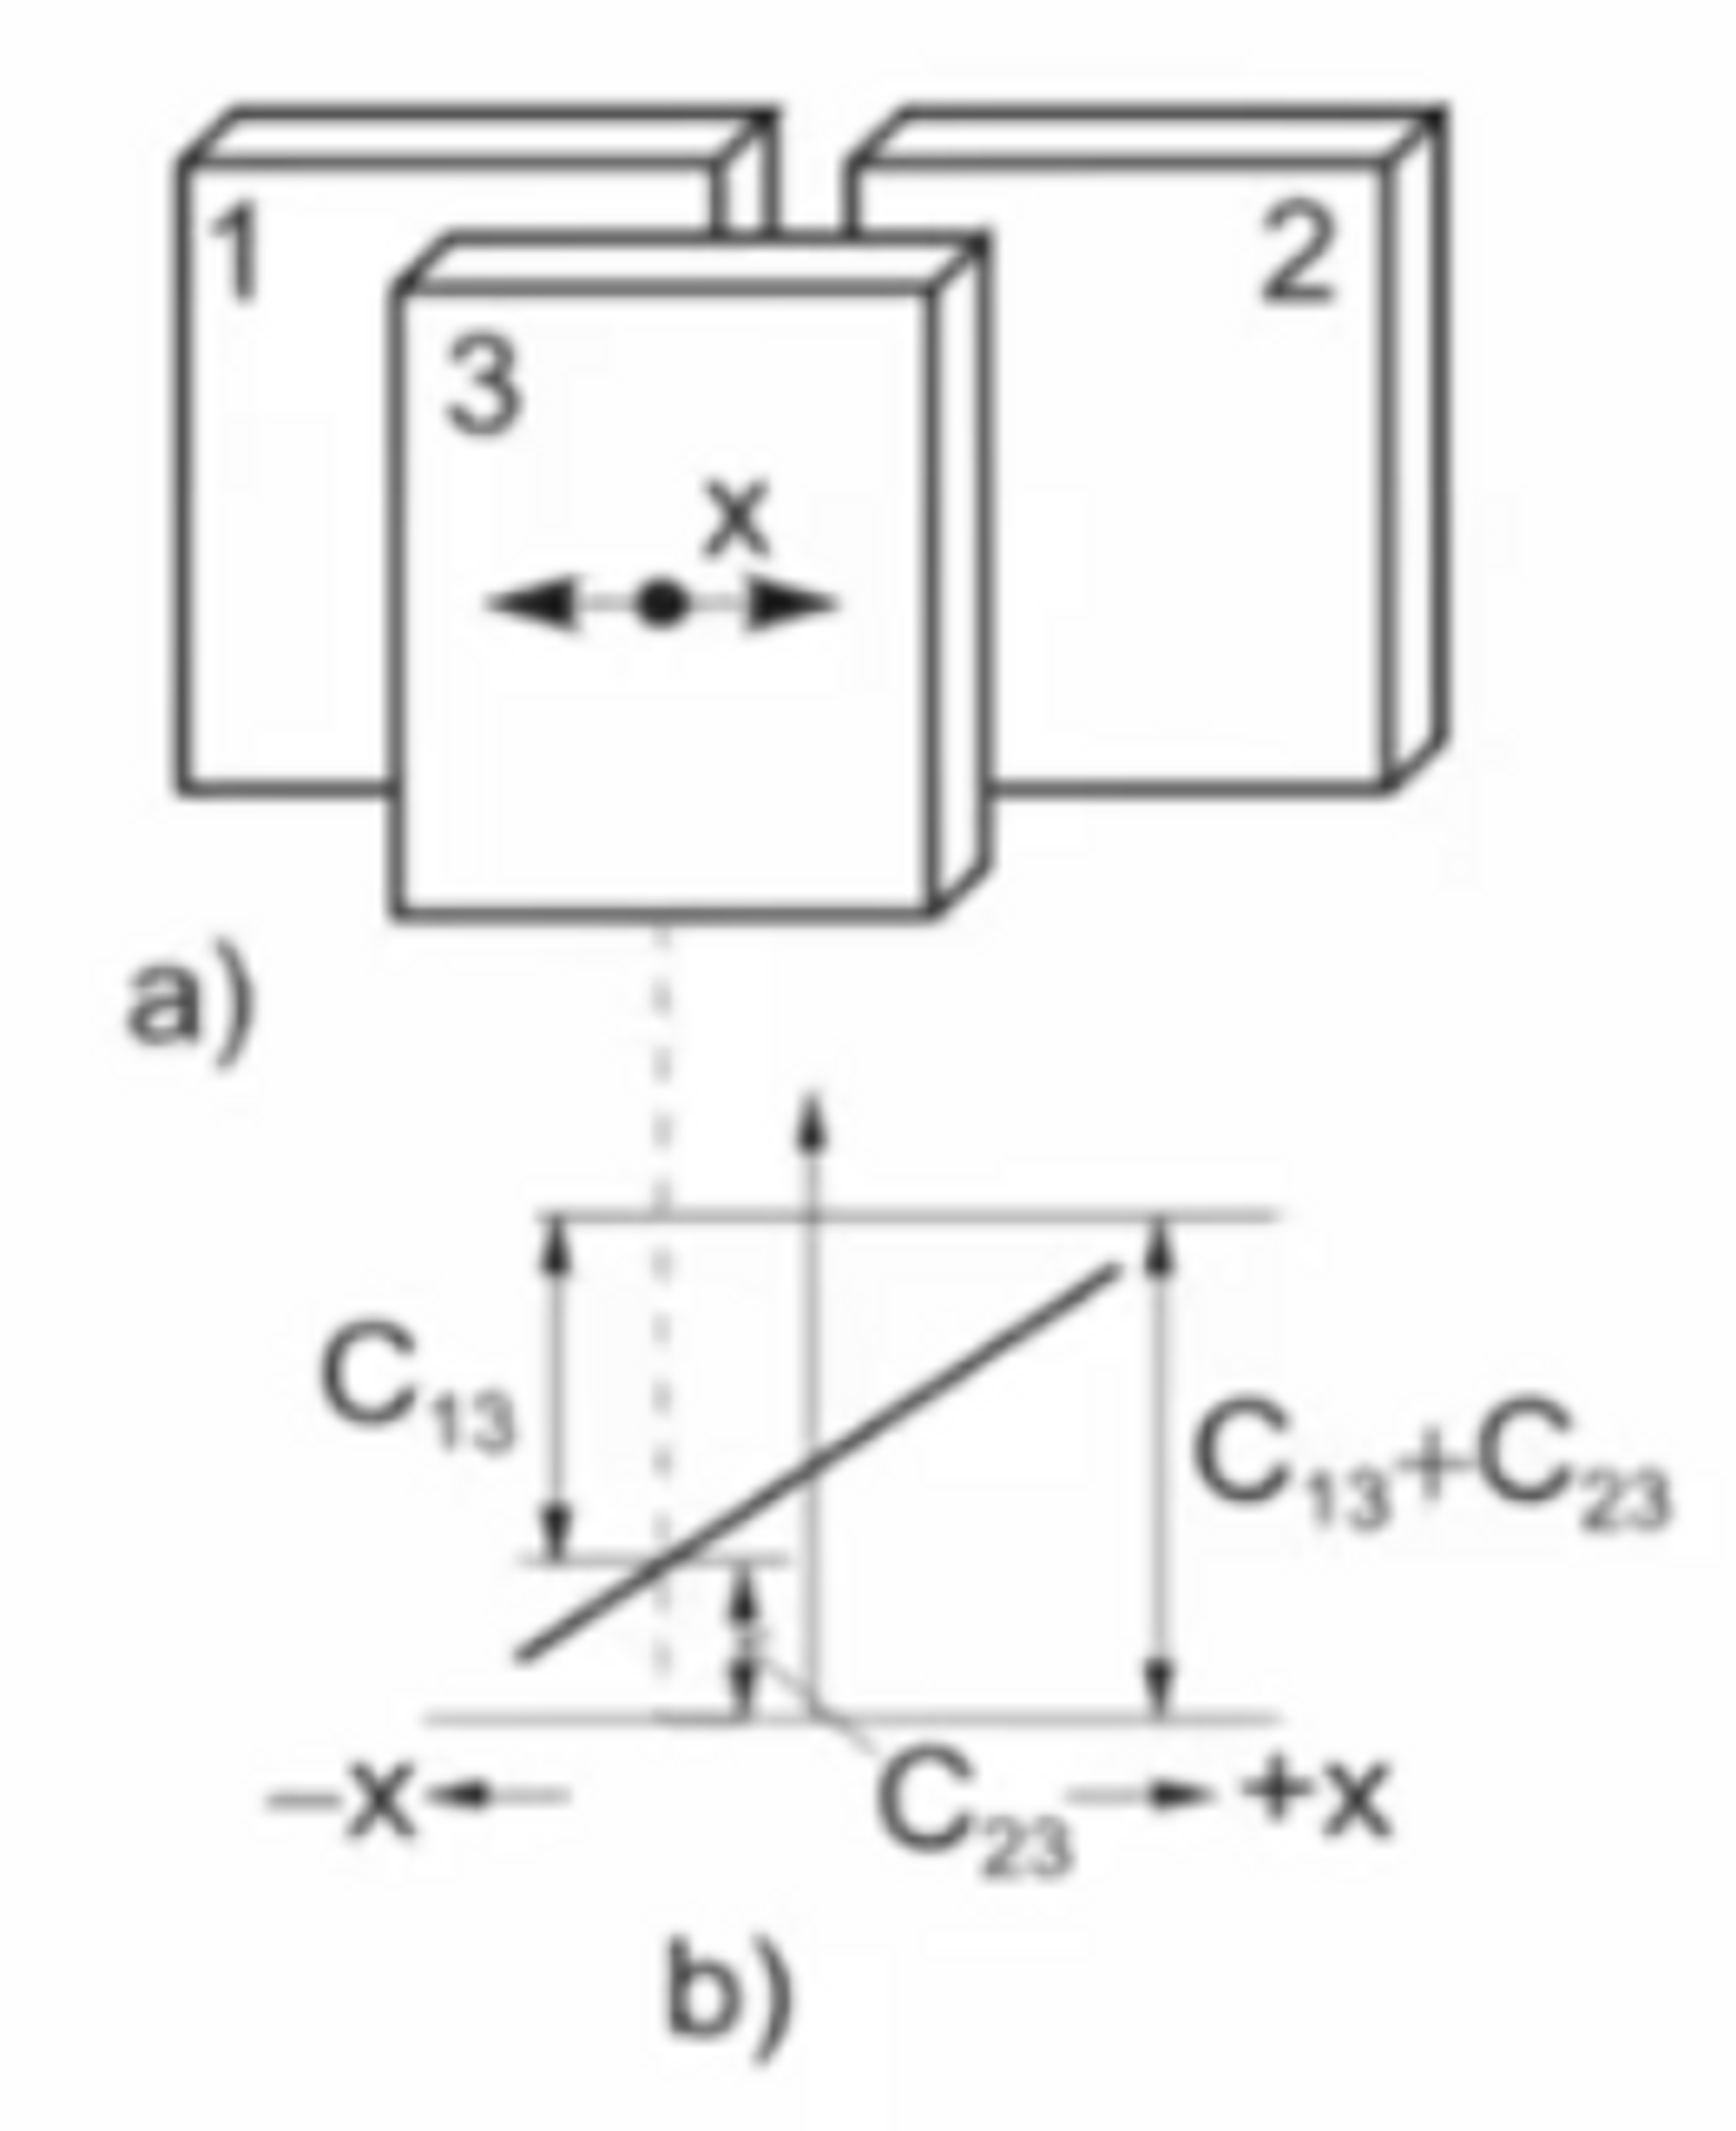
\includegraphics[scale = 0.07]{img/KapPromPloch.png}
\end{figure}

Vyhodnocení musí být provedeno v bezprostředné blízkosti elektrod. Kvůli malým kapacitám, se kterými se pracuje, by se projevoval vliv kabelů a naopak vliv elektrod by byl zanedbatelný.\\
Například v posuvném měřítku. V pevné části hodně elektrod a v posuvné jedna, kde díky změně kapacity měříme vzdálenost.\\

\subsubsection{Bezkontaktní snímače}
\begin{figure} [h!]
    \centering
    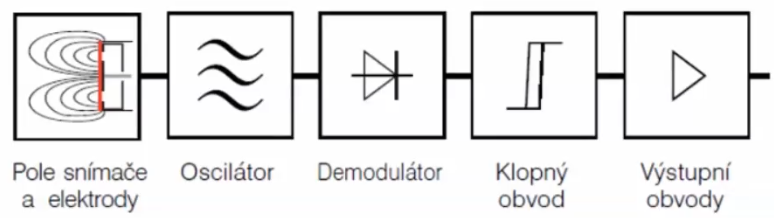
\includegraphics[scale = 0.3]{img/BezkonKap.png}
\end{figure}
Aktivní část tvoří 2 elektrody rovinného deskového kondenzátoru. Které jsou připojeny na oscilátor. Při přiblížení předmětu se naruší siločáry mezi deskami a změní se kapacita kondenzátorů a tím se změní i frekvence oscilátoru. Změna kmitočtu se vyhodnotí je vyhodnocena elektronikou snímače a je převedena na výstupní signál.\\
Toto funguje pro každý předmět, který má vyšší permitivitu než vzduch.\\
\begin{figure} [h!]
    \centering
    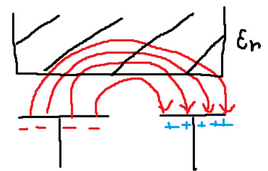
\includegraphics[scale = 0.5]{img/BezkontC.png}
\end{figure}

\subsubsection{Varianty}
\subsubsection*{Nevodivá clonka}
Změna kapacity je malá, mění se jen permitivita
\subsubsection*{Vodivá clonka}
Střední změna kapacity, mezi elektrody jakoby vkládáme další, která není uzemněna, když měníme vzdálenost, chová se to stejně, jak kdybychom zmenšovali vzduchovou mezeru - tj. bude se měnit kapacita(s velkou citlivostí) z důvodu změny vzdálenosti mezi elektrodami.\\
\subsubsection*{Vodivá clonka uzemněná}
Spojená s jednou s elektrod. Velká změna kapacity, výstupní kapacita je nepřímo uměrná vzdálenosti, 2x větší citlivost.\\

\begin{figure}[h!]
    \centering
    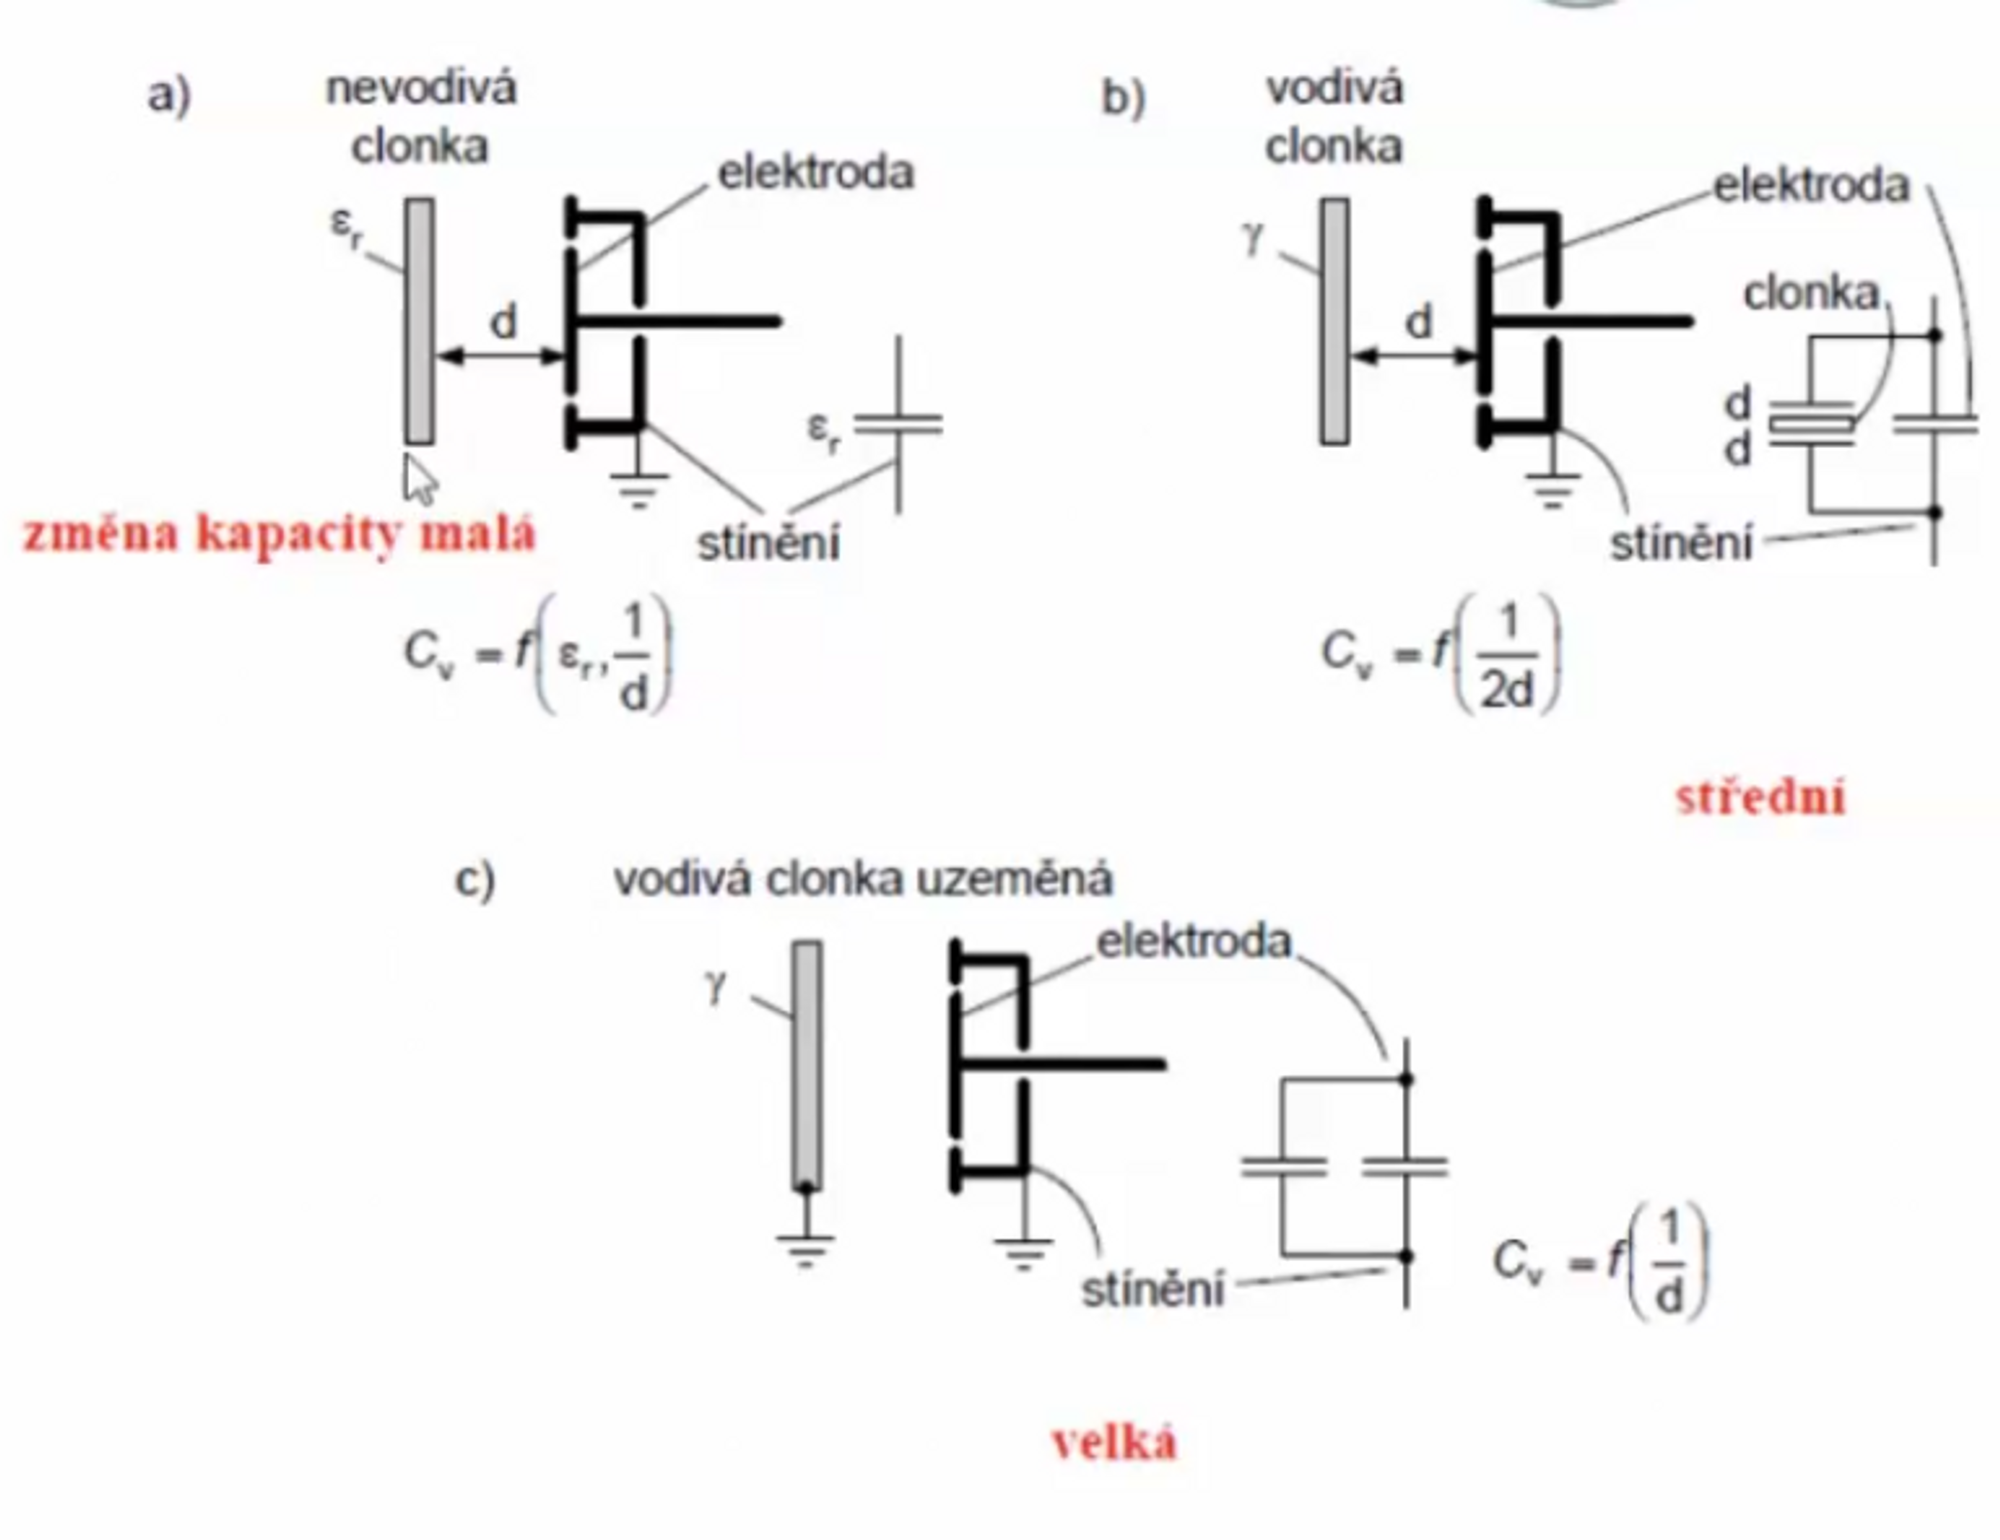
\includegraphics[scale = 0.2]{img/VariantyCpol.png}
\end{figure}
\subsubsection{Použití}
Měření hladiny vody, olejů, sypkých hmot přes stěnu nádrže.\\
Kontrola počtu/přítomnosti výrobků na balících linkách.\\


\section{Měření polohy - principy optické, magnetické, ultrazvukové}
\subsection{Optické snímače polohy}
Bezkontaktní měření polohy.\\
Poloha či její změna je detekována:
\begin{itemize}
    \item Změnou polohy zdroje světelného záření - polohy optické stopy
    \item Změna úhlu odrazu paprsku zdroje
    \item Interferencí zdrojového a odraženého paprsku
    \item Měření doby letu
    \item Zastínění nebo přerušení zdroje světla - optická závora
\end{itemize}

\subsubsection{CCD a CMOS obrazové snímače}
Maticové, řádkové.\\
Základem každého pixelu je fotodioda, pokud na ni dopadne záření, dojde ke generování páru elektron-díra a díky fotoelektrickému jevu se objeví na fotodiodě napětí. Čím větší intenzita záření, tím větší generované napětí.\\
Řádkové mají výhodu vysoké rychlosti vyčítání, rychlá detekce změny polohy paprsku. Maticové mají výhodu měření změny ve 2 osách.\\
Kritické parametry: šum a rozměr fotodiody.\\
CMOS snímače nejčastěji, díky ceně a výkonu.\\
\begin{figure}[h!]
    \centering
    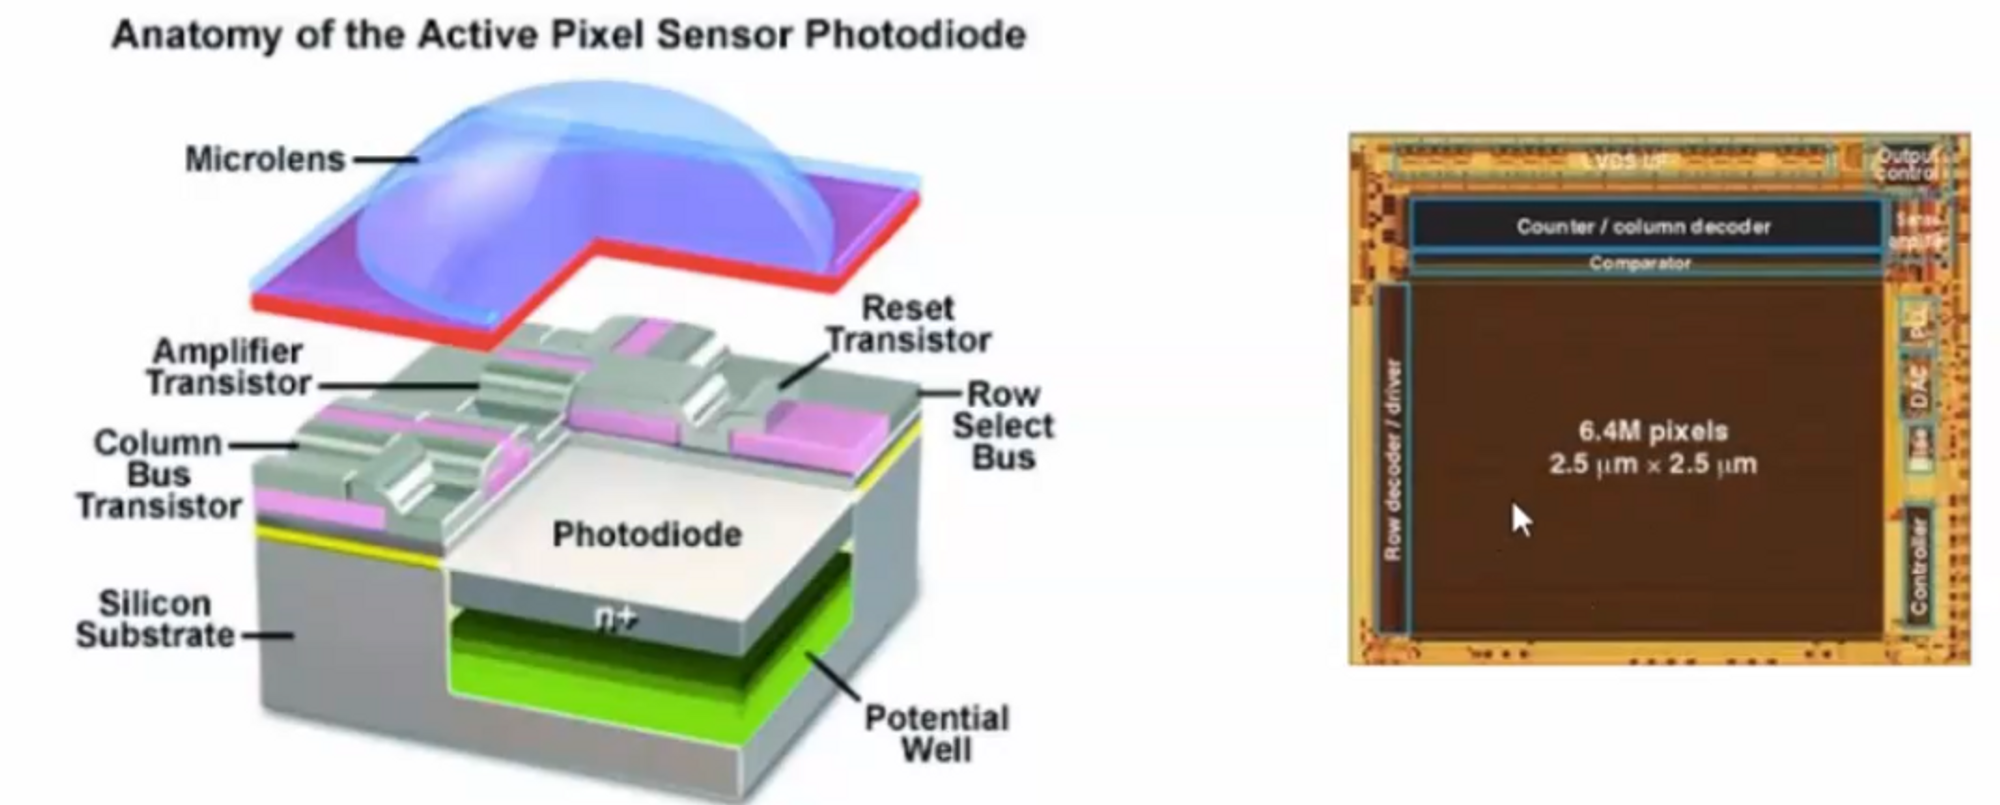
\includegraphics[scale = 0.2]{img/CMOS.png}
\end{figure}

Využití:
\begin{itemize}
    \item Přímé měření rozměrů
    \item Triangulační snímače
    \item Snímače clonícího typu
\end{itemize}

\subsubsection{Trianguční snímač vzdálenosti}
Princip: zdroj světla, typicky laser či fotodioda, jeho paprsky jsou pomocí čoček fokusovány do svazku. Svazek pak dopadá na předmět, jehož vzdálenost chceme detekovat, na předmětu dojde k difúznímu odrazu a my pomocí čoček tento odraz koncentrujeme na plochu řádkové kamery, při pohybu předmětem se nám bude pohybovat i poloha odraženého paprsku.\\
Využívá se známé vzdálenosti detektoru a vysílače a trojúhelníku mezi čočkou a rozměrem CMOS čipu. Využije se podobnosti trojúhelníků předmět, detektor, vysílač a čočky a krajů detektoru.\\
Rozlišení od jednotek mikrometrů po desítky milimetrů.\\
\begin{figure}[h!]
    \centering
    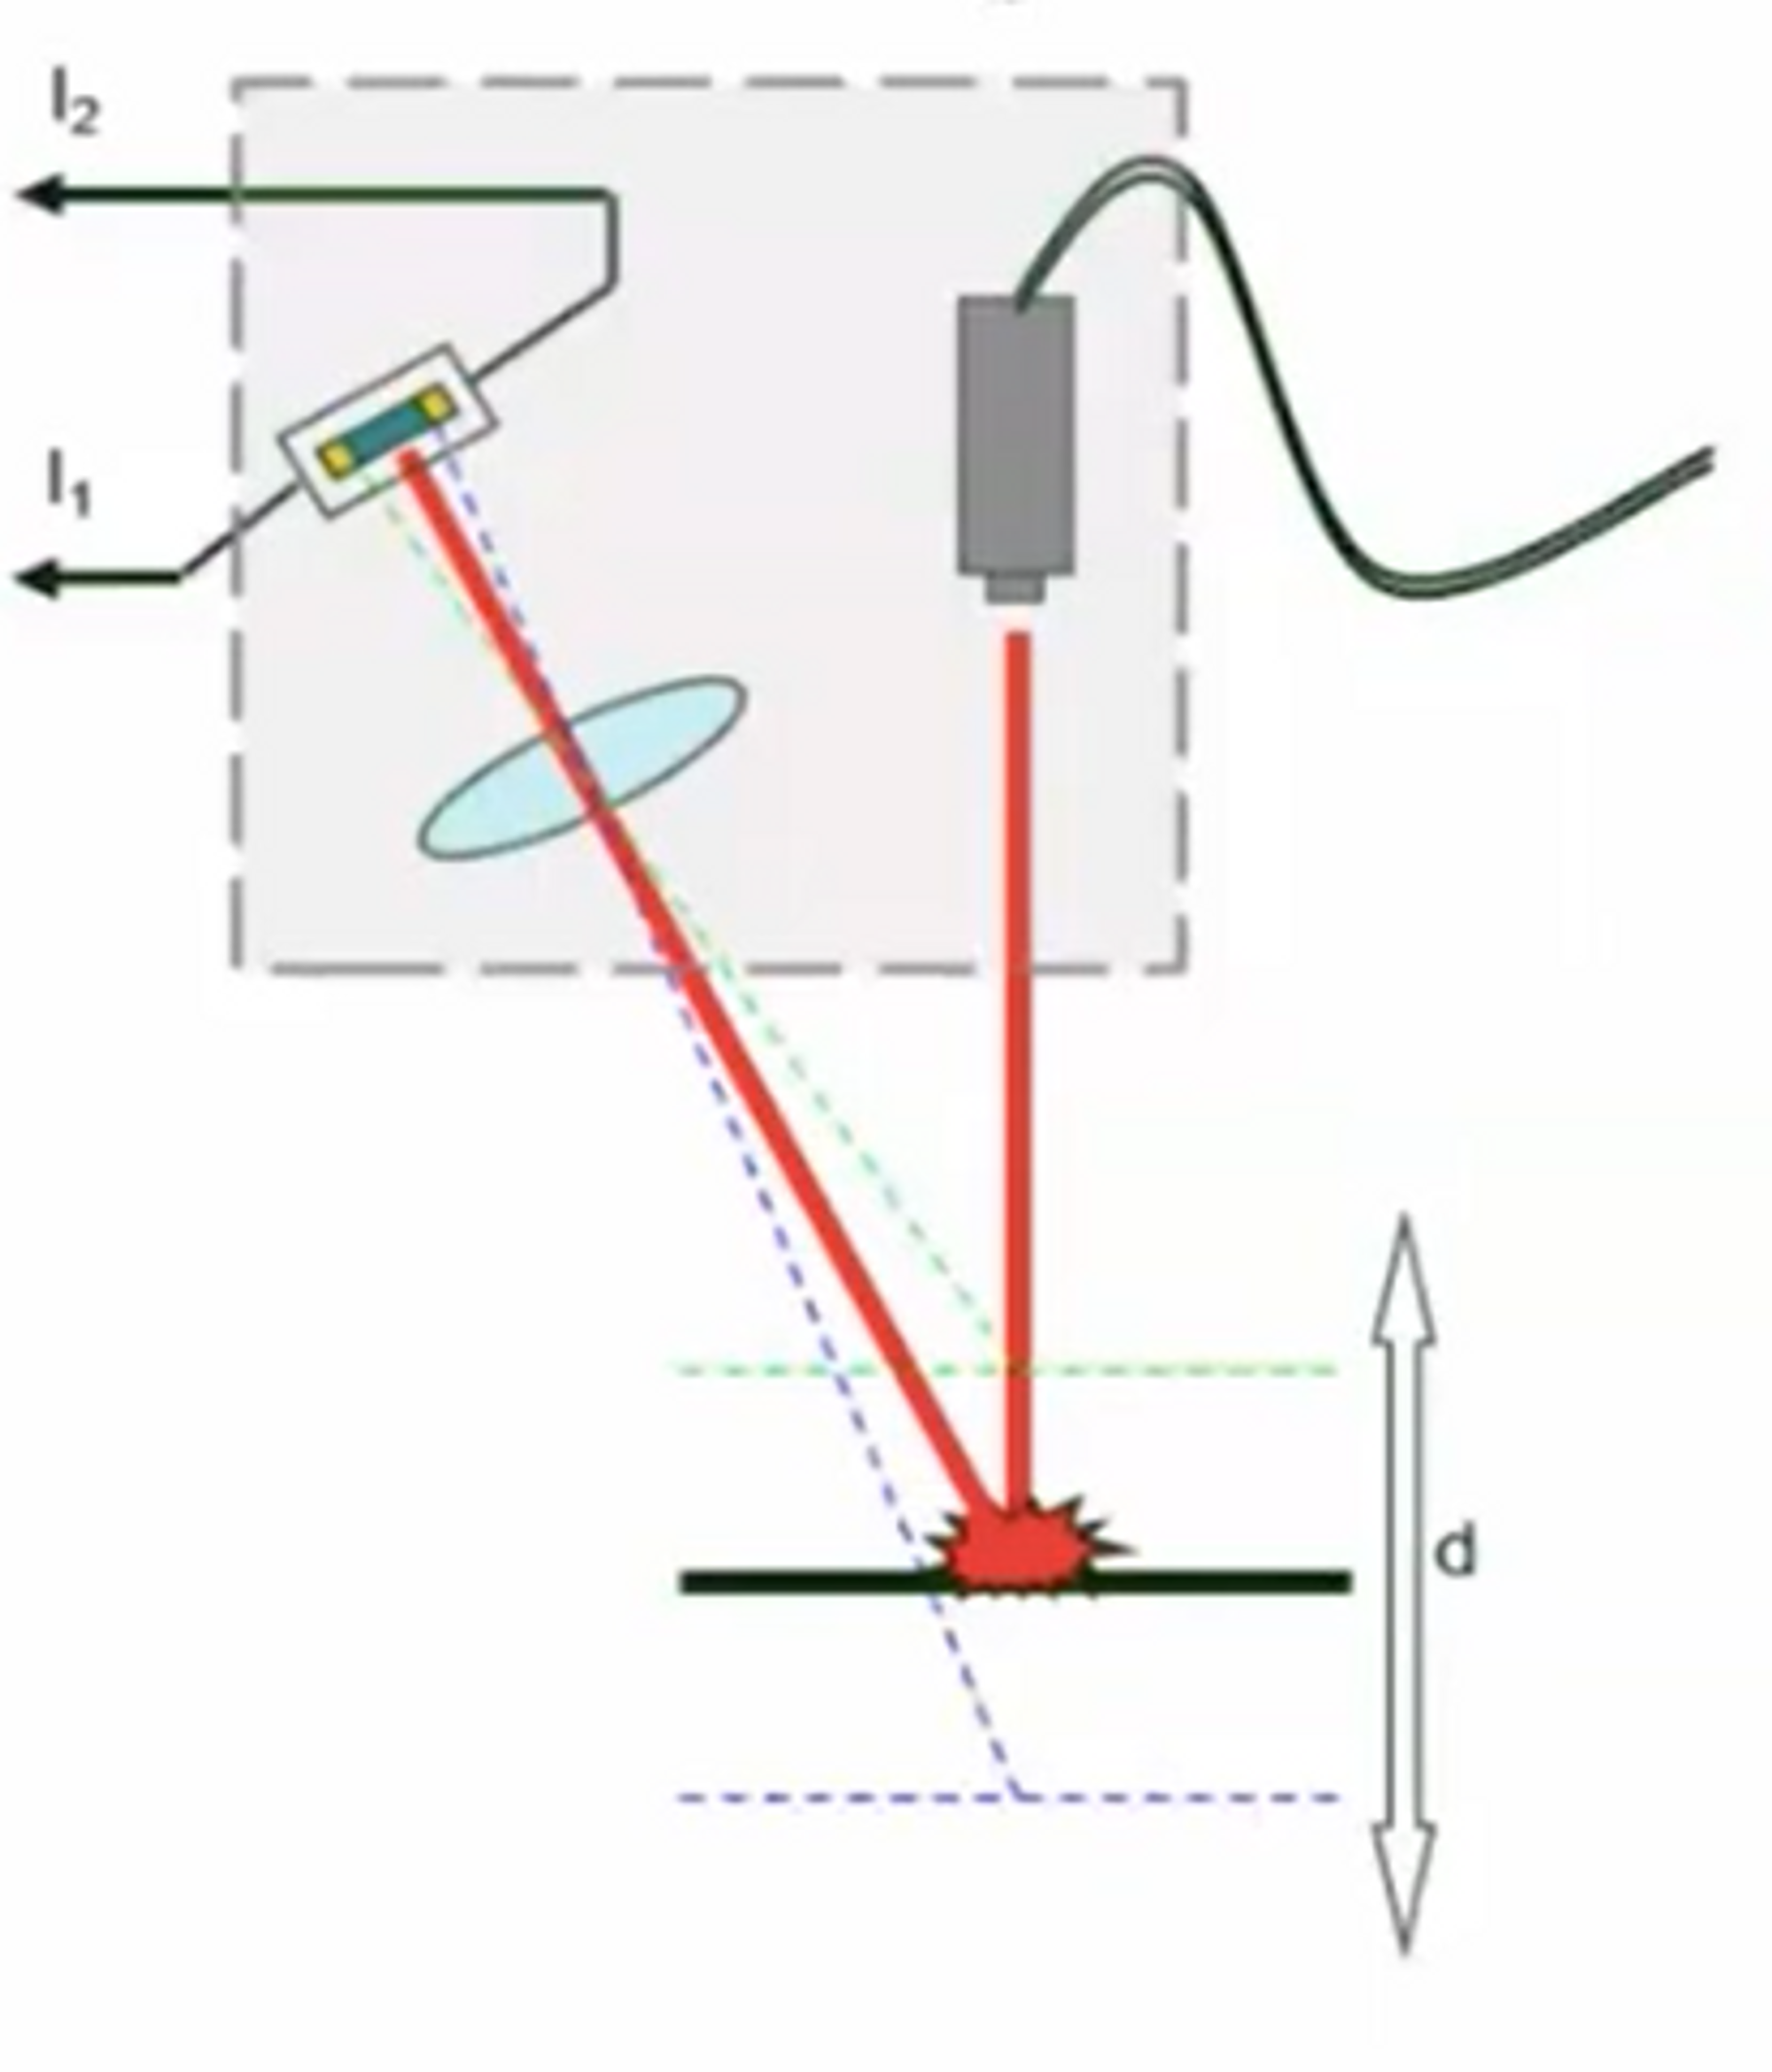
\includegraphics[scale = 0.1]{img/Triang.png}
\end{figure}

\subsubsection{Inkrementální snímač}
Kontaktní snímač, abychom mohli snímač použít, musíme mít clonku spojenou s pohybujícím se předmětem.\\
Například v servomechanizmech. Pro přesné nastavení úhlu.\\
Také označován jako optická enkodér.\\
Max rozlišení \(0.05\mu m\), 1" nutné držet správnou geometrii.\\
Princip: Pohybující se clonka s ryskami(uchycená na hřídeli, otáčí se) a nad ní je pevní clonka s kukátkem(součástí statoru). Na jedné straně jsou pak diody, jako zdroj světla a na druhé straně jsou příjmací fotodiody. Clonky jsou 2, vzájemně posunuté o čtvrt rozestupu rysek na hlavní clonce. V každé clocne jsou 2 kukátka vzájemně posunuta o 180°. Clonky jsou 2 kvůli určení směru otáčení, pokud by byla jedna můžeme detekovat otáčení, ale jeho směr. Pokud se pohybujeme po směru hodinových ručiček, pak signál A předbíhá o čtvrt periody signál B, pokud proti směru, pak B předbíhá A.\\
Refereční značka používána pro určení polohy.\\
\begin{figure}[h!]
    \centering
    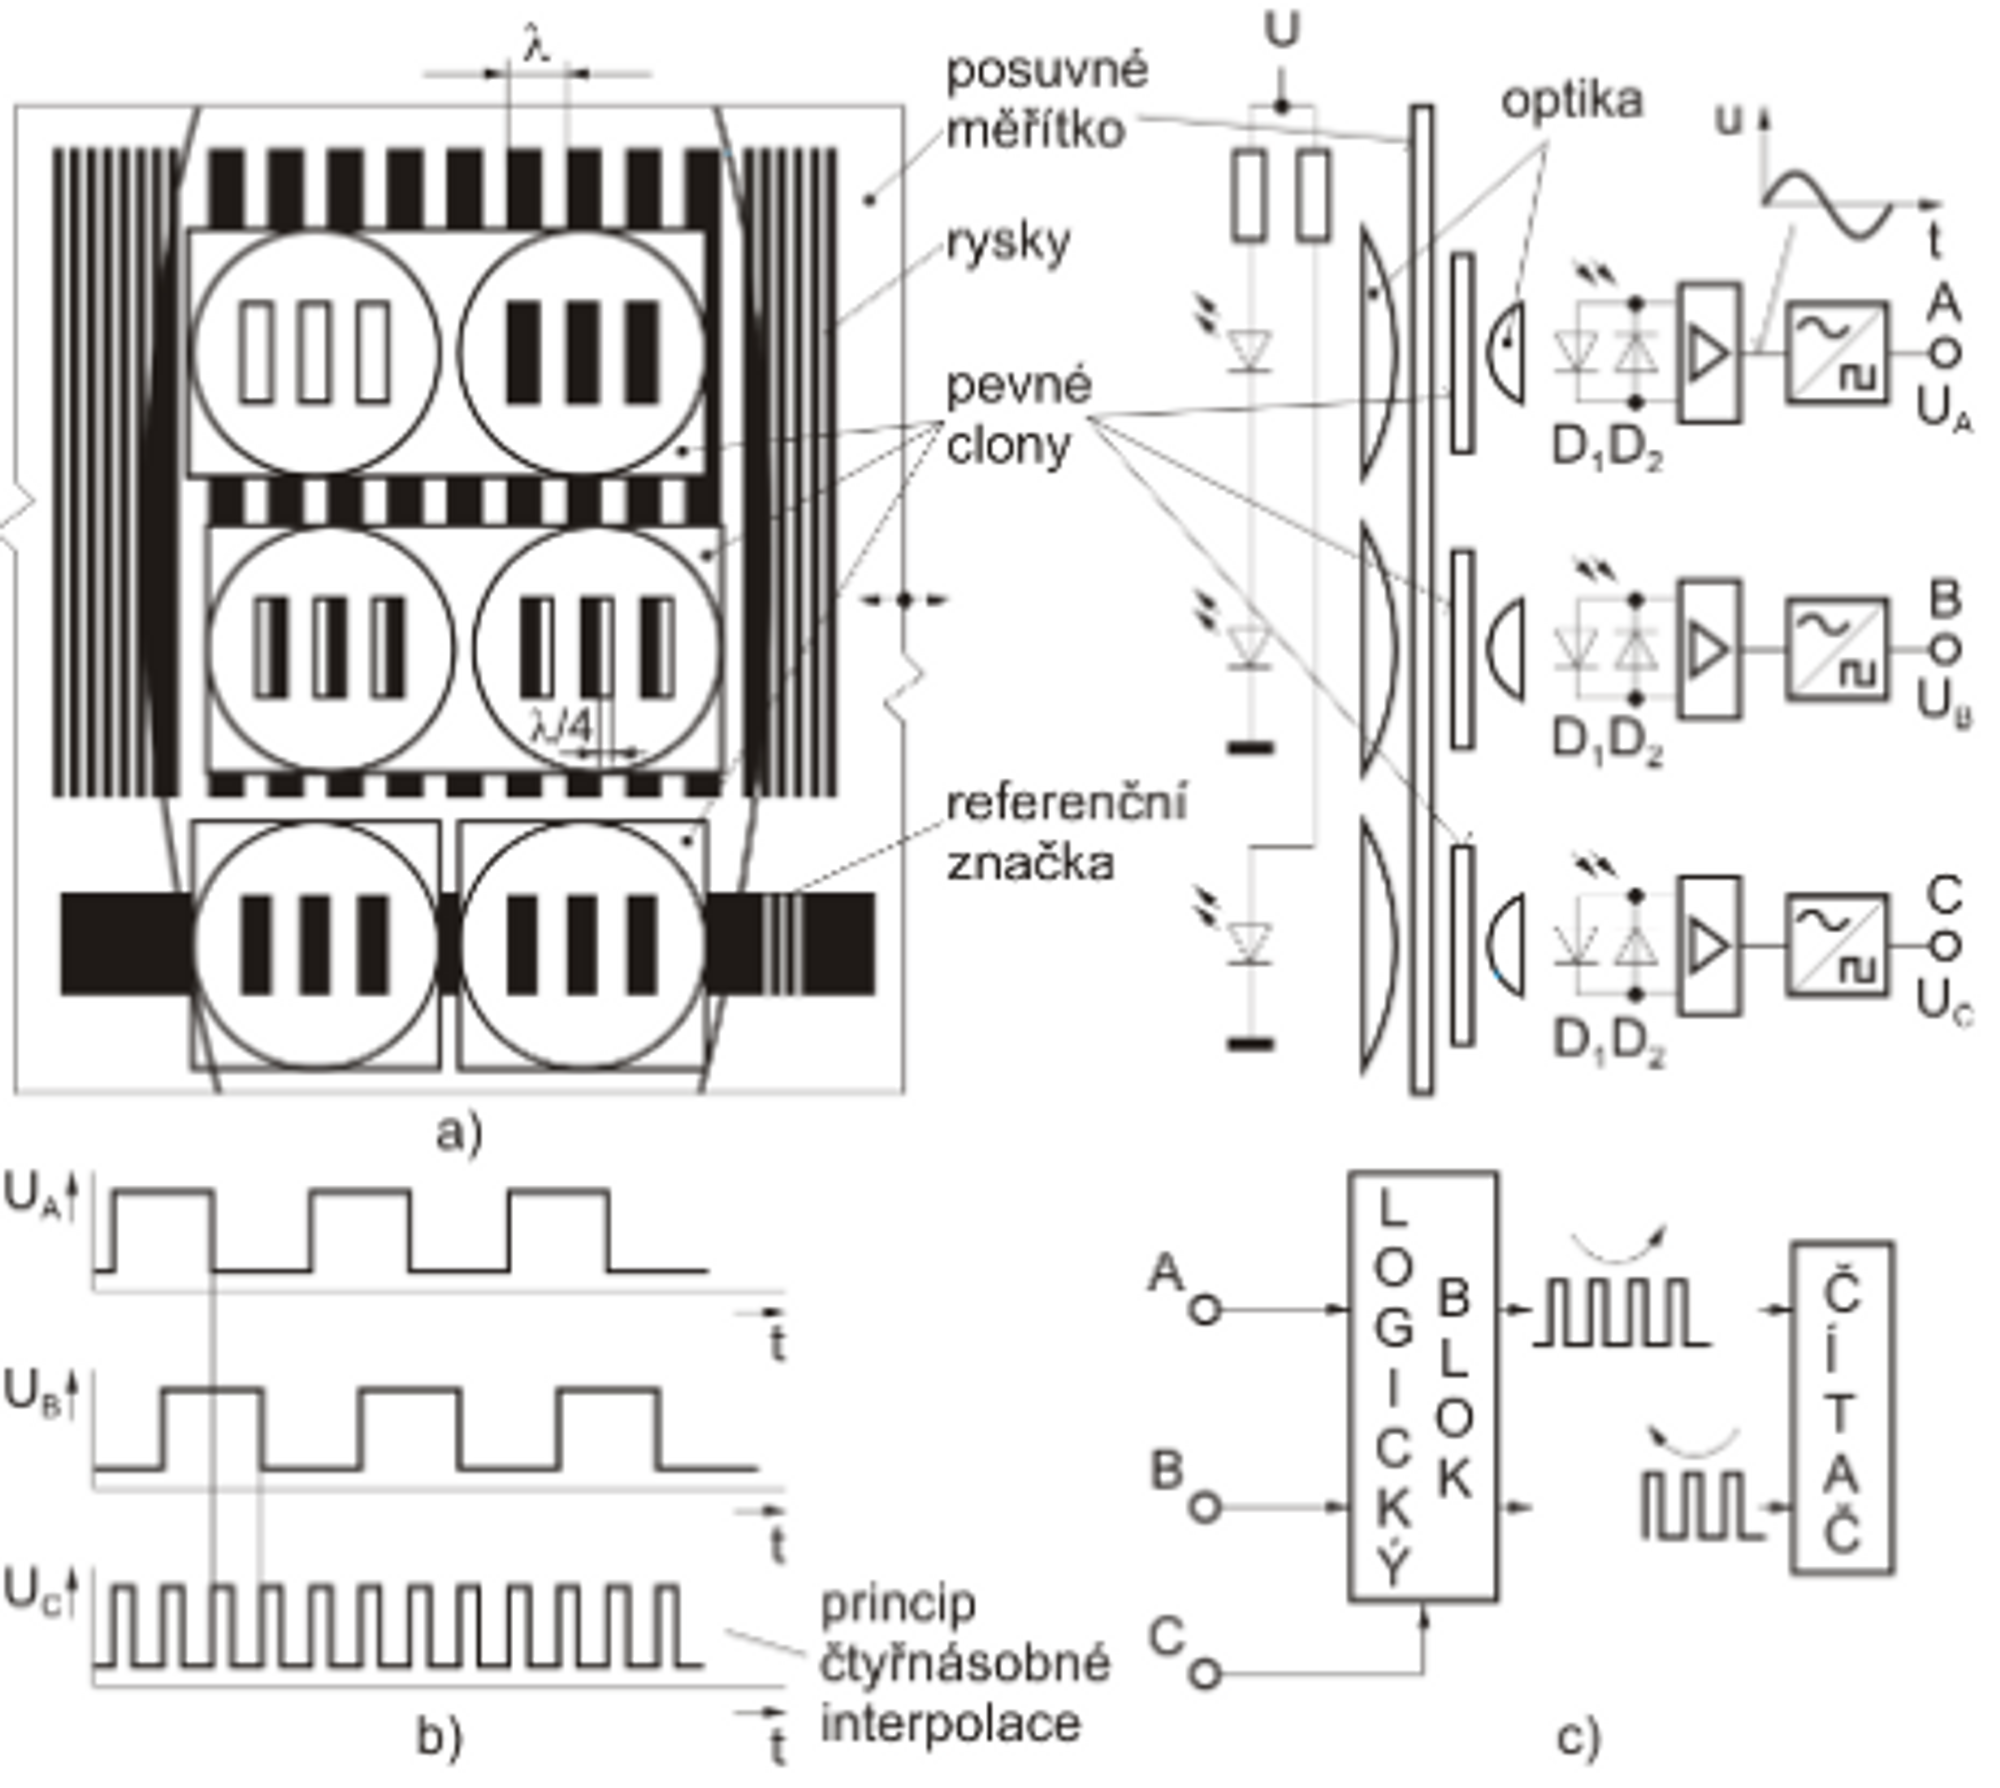
\includegraphics[scale = 0.1]{img/Inkrem.png}
\end{figure}
Od stovek impulzů na otáčku až po desítky tisíc impulzů na otáčku. Při vysokých rozlišeních se řeší interpolací.\\
\newpage
\subsubsection{Snímače polohy s prostorovým kódem}
Pro lineární i rotační posun.\\
Výhoda, pokud vypadne napájení tak i přes to víme podobu.\\
Ze snímače dostáváme ne impulsy, ale bitové slova, které odpovídá absolutní poloze.\\
V grayově kódu či PRC(pseudo random code). Mění se pouze jeden bit při přechodu z jednoho stavu do druhého.\\
Rozlišení 4 až 17 bitů, nejčastěji 8-12b.\\
\begin{figure}[h!]
    \centering
    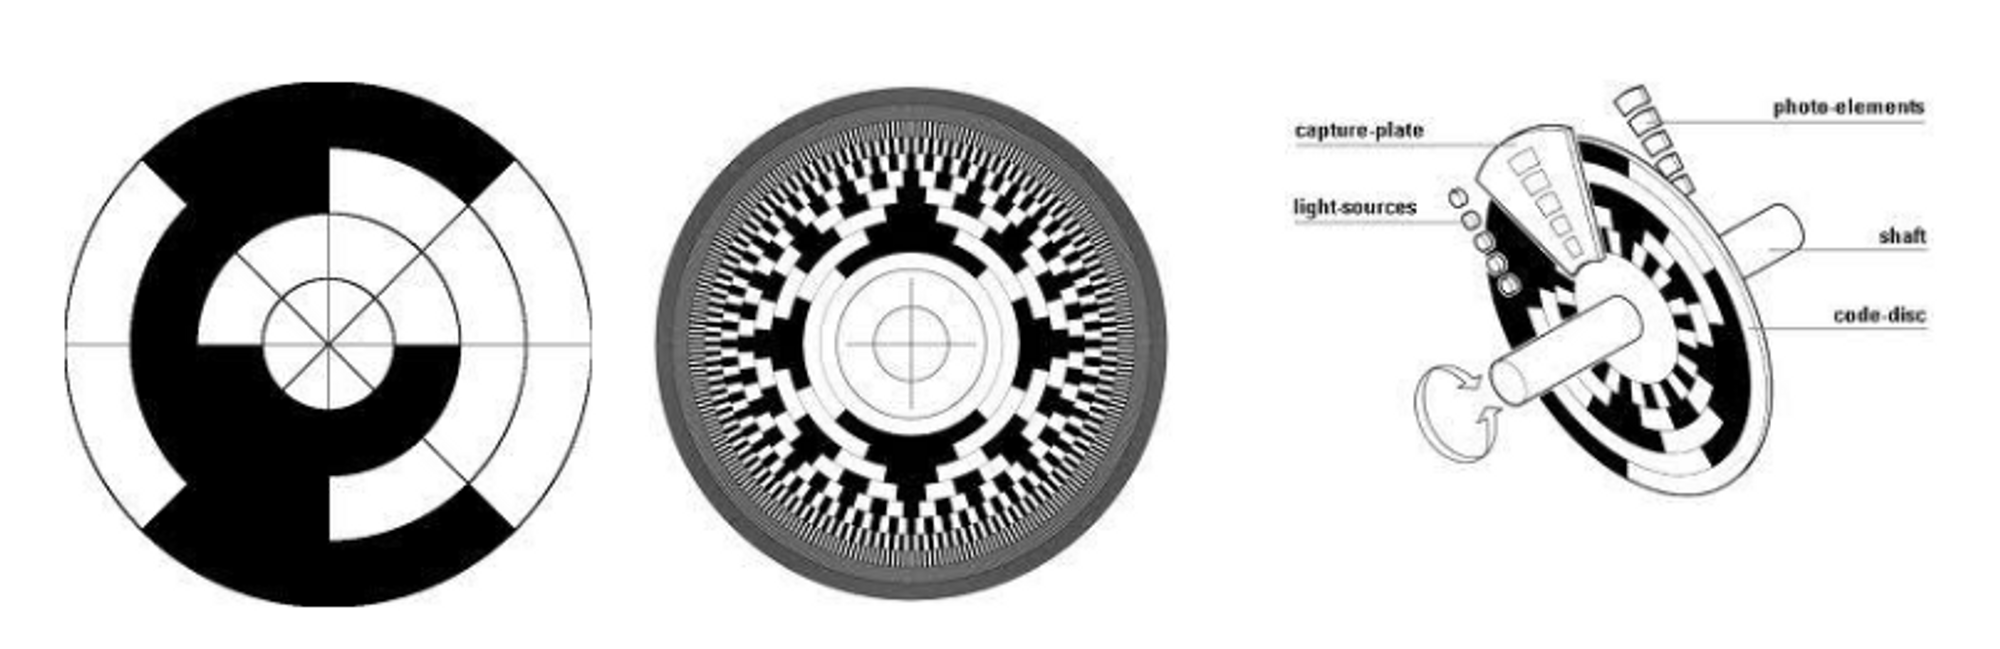
\includegraphics[scale = 0.2]{img/ProstKod.png}
\end{figure}

\subsubsection{Interferometrické snímače}
Základní princip Michelsonův interferometr. Máme referenční optickou trasu a měřící trasu, které jsou různě dlouhé a díky tomu, že jsou různě dlouhé, tak dochází k interferenci zdroje koherentního záření. \\
Princip pro debily: Máme zdroj koherentního záření, typicky helium-neonový laser, na pevné vlnové délce. To že je koheretní znamená, že se nemění fáze a frekvence v čase a prostoru. Tato sinusovka dopadne na polopropustné zrcátko, které polovinu propustí a polovinu odrazí, takže polovina paprsku dopadne na měřící zrcadlo(součástí pohybujícího se předmětu), které má vlastnost, že ať se na něj z kamakoliv posvítí, odrazí se to zpátky stejnou cestou. Takže se to vrací na polopropustné zrcátko, takže čtvrtina se odrazí do detektoru. Druhá polovina jde do referenčního zrcadla a stejně tak se polovina z této části dostane na detektor. Detektor je obyčejná fotodioda na kterou dopadá záření, v podstatě jsou to 2 sinusovky, které na něj dopadají. Pokud by byla vzdálenost obou zrcadel přesně stejná, dopadnou se stejnou fází a jejich energie se sečte(konstruktivní interferometrie) a intenzita záření se zdvojnásobí. Pokud je rozdíl vzdálenosti zrcadel násobkem vlnové délky záření, také dopadnou se stejnou fází. Pokud jsou mimo tyto pozice, tak se fáze rozchází, sinusovky se budou sčítat, ale nedostanou se na maximální hodnotu, pokud jsou posunuty tak, že okamžité hodnoty jsou jedna v maximu a druhá v minimu, dojde k destruktivní interferometrii a intenzita světla bude nulová.\\
Když tedy pohybujeme zrcadlem, dostanem harmonický signál se vzdáleností maxim poloviny vlnové délky záření. Na výstup se dá čítač, který tyto maxima počítá a tím se určuje vzdálenost.\\
\begin{figure}[h!]
    \centering
    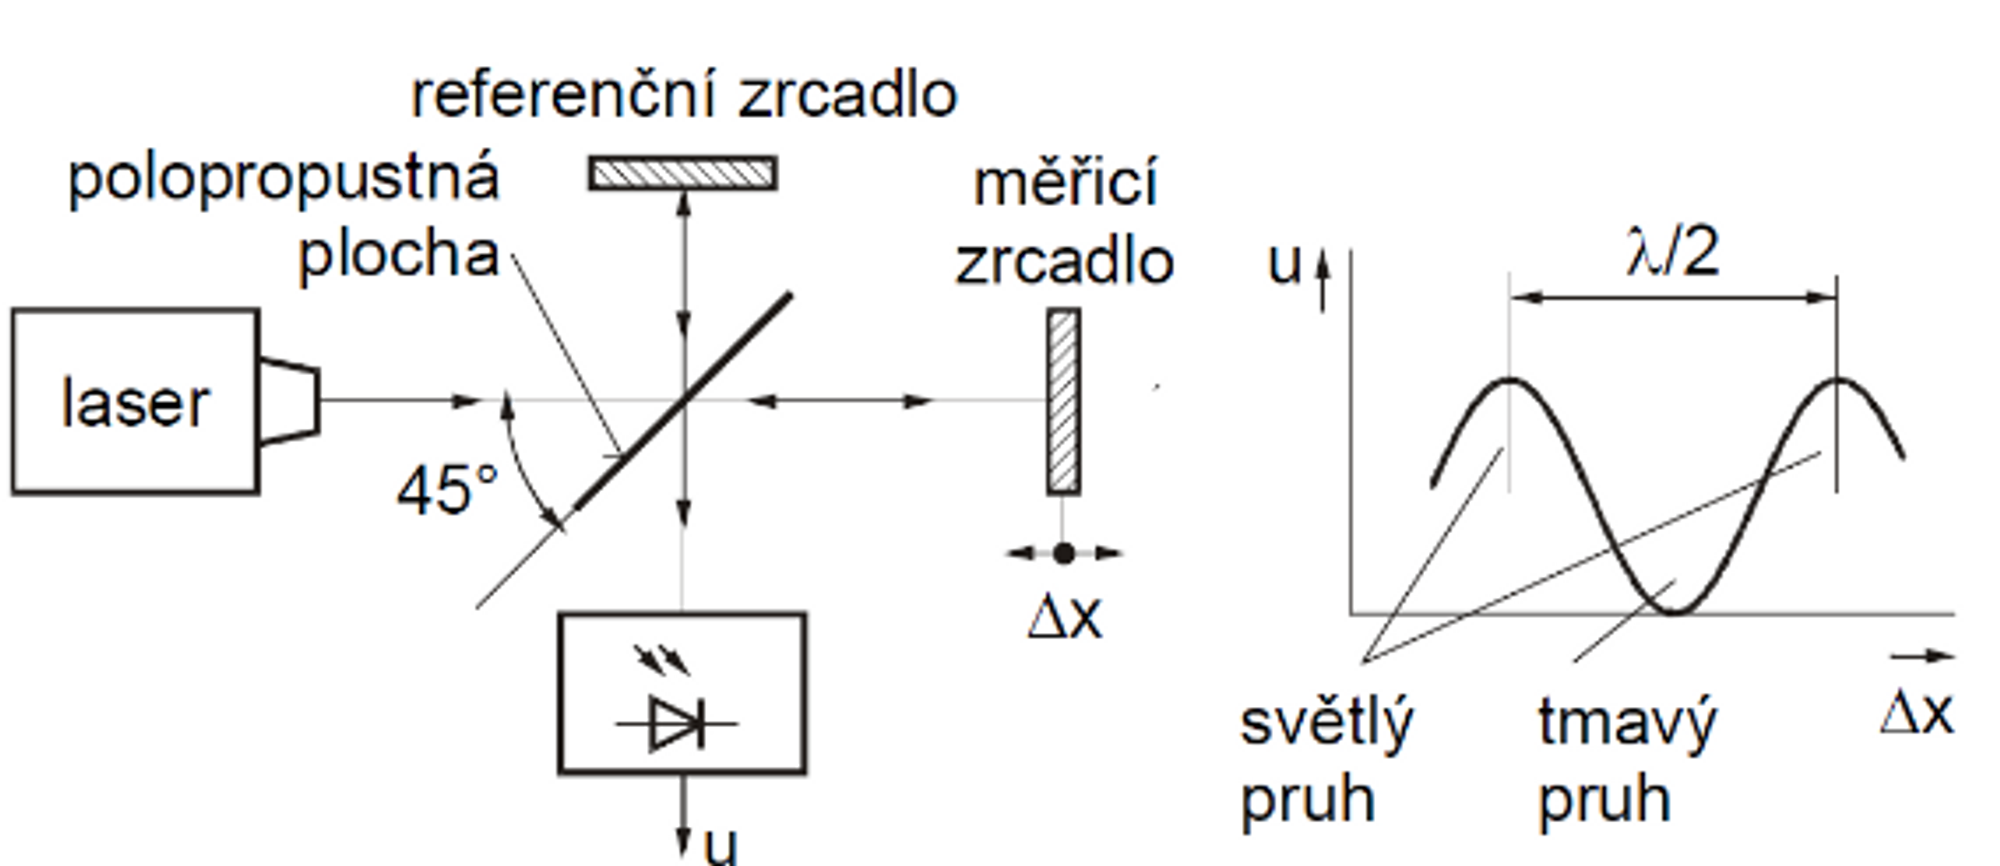
\includegraphics[scale = 0.2]{img/InterfSnim.png}
\end{figure}

Nevýhoda je, že nepoznáme směr pohybu. Řeší se stejně jako u inkrementálního, posunem o čtvrt periody.\\
Záření vracející se do laseru by mohlo být problém, pro se před něj umisťuje jednosměrně propustné zrcátko.\\
Pro zvýšení přesnosti a rozlišení Laser Doppler Interferometer - signál se moduluje a vyhodnocuje se nejen fázový posun, ale také posuv ve frekvenci daný dopplerovým jevem. Pohyb od nás, kmitočet se snižuje, pohyb k nám kmitočet se zvětšuje. Těleso však musí být v pohybu. Je schopen měřit na pikometry, oproti klasickým na nanometrech.\\

\subsubsection{Měření doby letu}
Vyšleme optický impulz a měříme dobu za jakou se vrátí. \\
Problém s rychlostí. Vyšleme amplitudově nebo frekvenčně modulovaný signál, posunem měřený kmitočet, takže měříme fázový rozdíl časově posunutého signálu s modulací

\begin{figure}
    \centering
    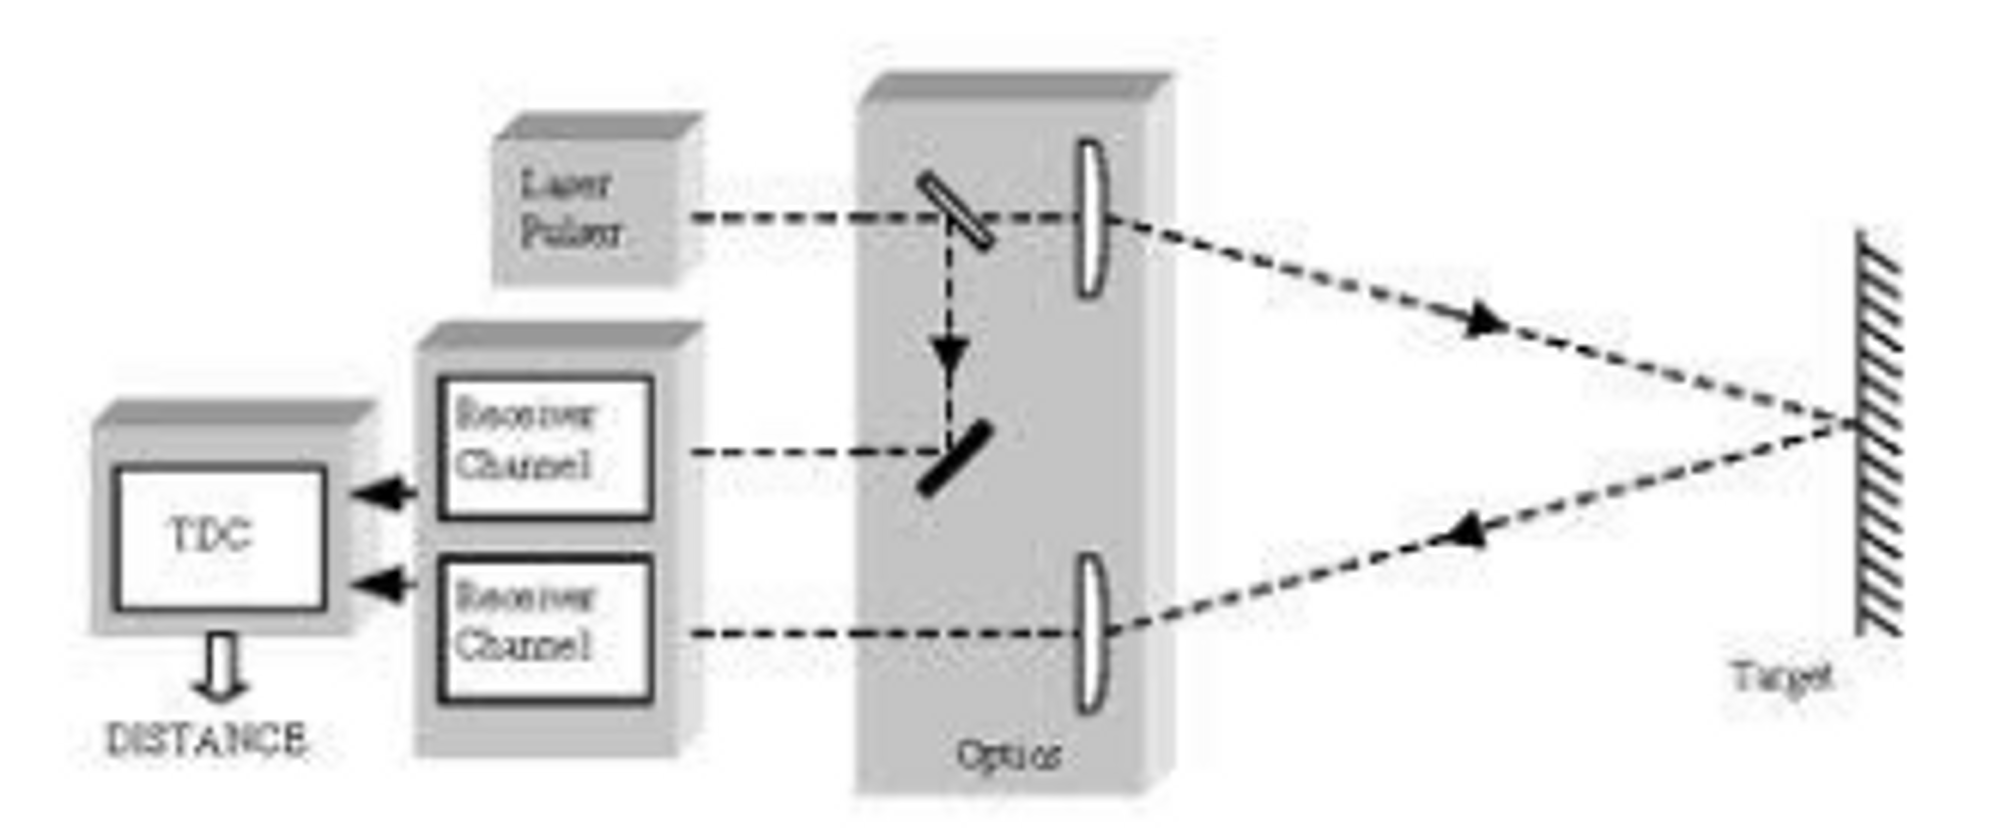
\includegraphics[scale = 0.1]{img/TOF.png}
\end{figure}

Dá se použít i pro velmi velké vzdálenosti, použila se pro měření vzdálenosti země měsíc.\\

\subsection{Magnetické snímače polohy}
\subsubsection{Hallův snímač}
Využívá Hallova jevu. Máme destičku z vodivého materiálu a když tou destičkou prochází elektrický proud a umístíme ji do magnetického pole, dojde k vychýlení nosičů náboje kolmo k směru jejich pohybu skrze vodič, k tomuto vychýlení dochází pomocí Lorentzovy síly. Tento přesun nosičů do jedné části destičky vyvolává rozdílný potenciál na jejích krajích. Což můžeme měřit jako takzvané Hallovo napětí. \\

\begin{center}
    \(U_H = k_H \frac{I_p \cdot B}{d}\)
\end{center}
Kde k je materiálová konstanta, I je proud procházející elektrický proud, d je tloušťka materiálu destičky, B je magnetická indukce.\\
Destička je tvořena tenkou vrstvou monokrystalu polovodiče InAs, InSb, Si, GaAs. \\
\begin{figure}[h!]
    \centering
    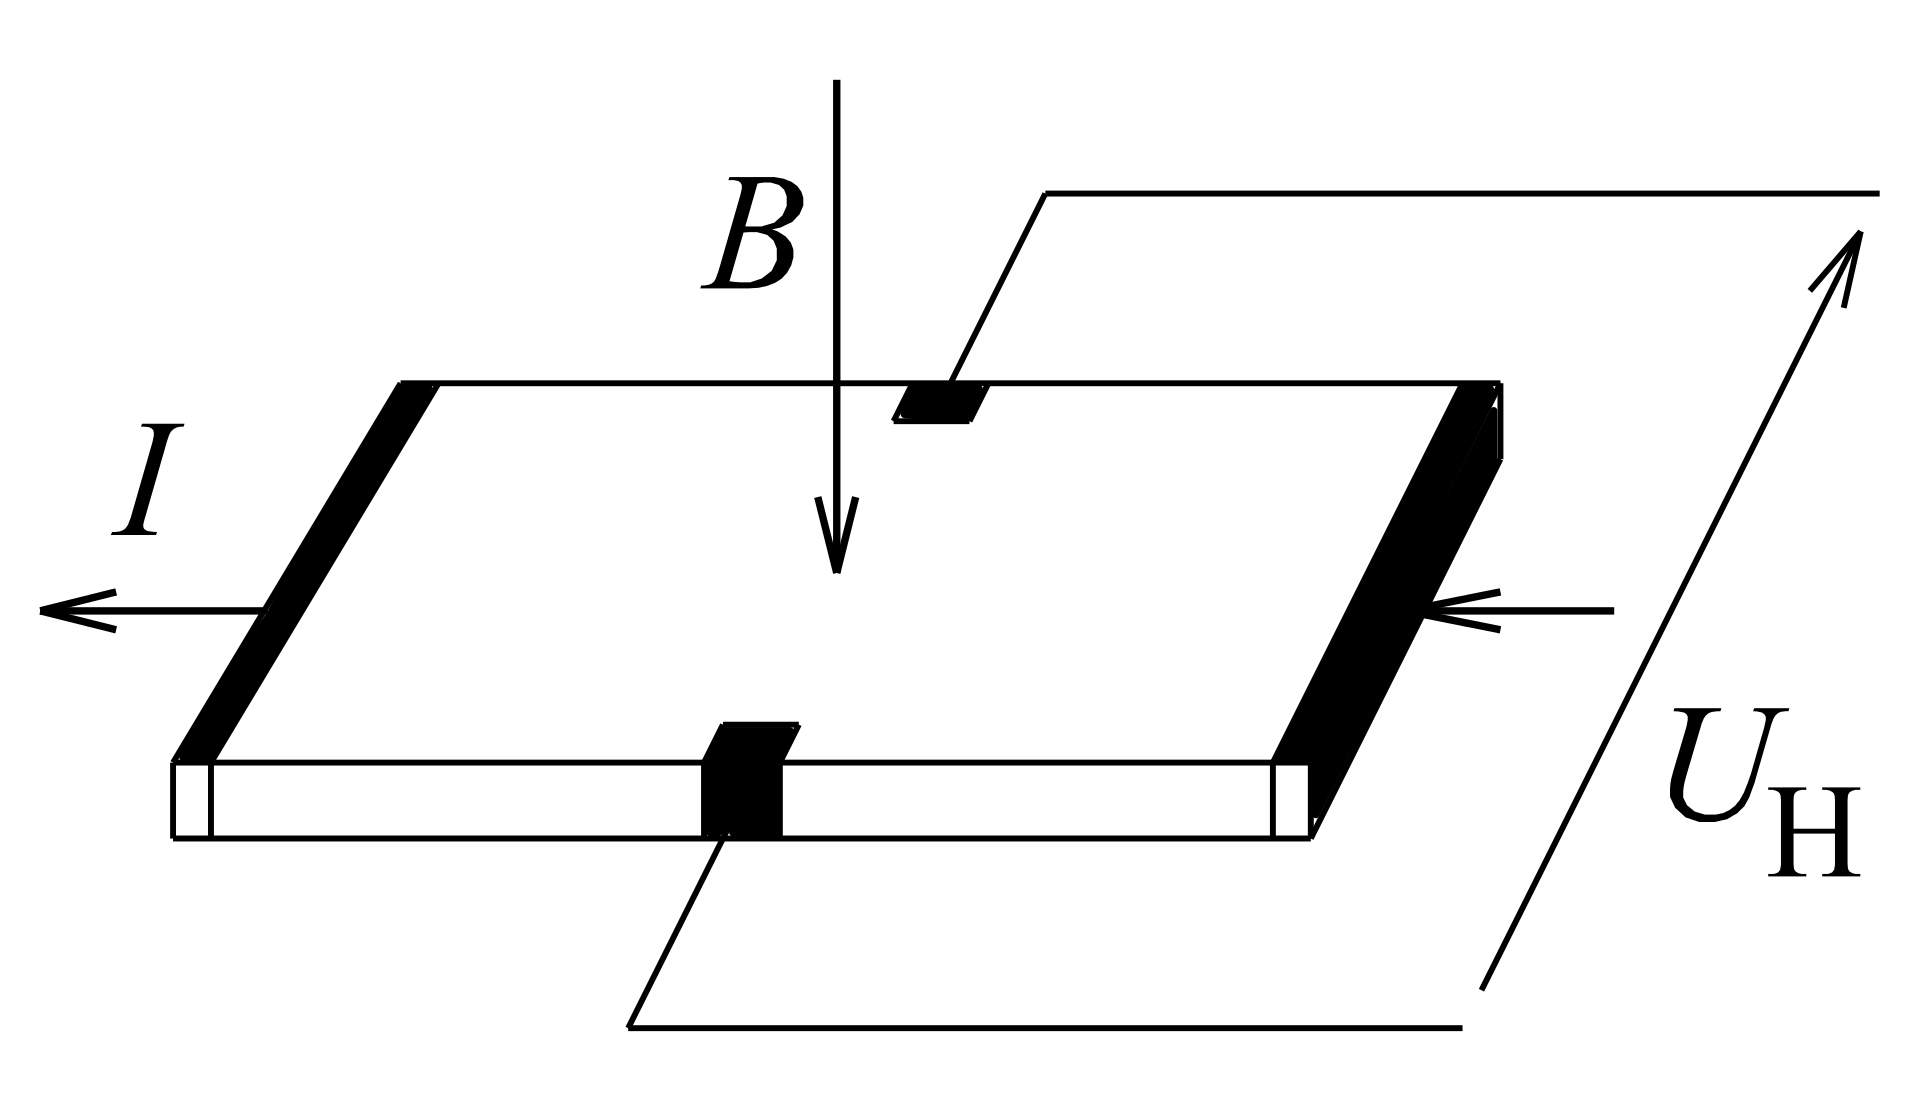
\includegraphics[scale = 0.07]{img/HallSonda.png}
\end{figure}
Konstanta, tloušťka, proud se nemění a výstupní napětí je přímoúměrné působícímu magnetickému poli/indukci. Tím pádem můžeme detekovat zdroj magnetického pole, případně jeho vzdalování.\\
Bezkontaktní měření polohy nebo otáček.\\

\subsubsection{Magnetorezistor}
AMR - anizotropní magnetorezistance.\\
GMR - Gigantická magnetorezistance.\\
TMR - Tunelová magnetorezistance.\\
Citlivější, vyhodnocujeme změnu odporu.\\
Magnetorezistivní jev: Na nevodivém stubrtrátu nanesena vodivá vrsta. Tato vrsta se skládá ze dvou částí. Niklových jehliček, které mají dobrou vodivost a mezi nimi je polovodivá vrstva. V podstatě máme mnoho halových sond v sérii za sebou. Na začátku se elektrony rovnoměrně rozmístí, protože se odpuzují. Po přivedení proudu se elektrony rozběhnou a magnetickým polem jsou pomocí lorentzovy síly vytlačovány jedním směrem, tím jak velká je intenzita tohoto pole určujeme velikost průřezu vodiče. Elektrony doběhnou na další vodivou vrstu, kde se opět srovnají a cyklus jde znova.\\
Toto se navenek projevuje jako elektrický odpor v závislosti na intenzitě magnetického pole.\\
Slabá citlivost - malé změny odporu.\\
\newpage
\begin{figure}[h!]
    \centering
    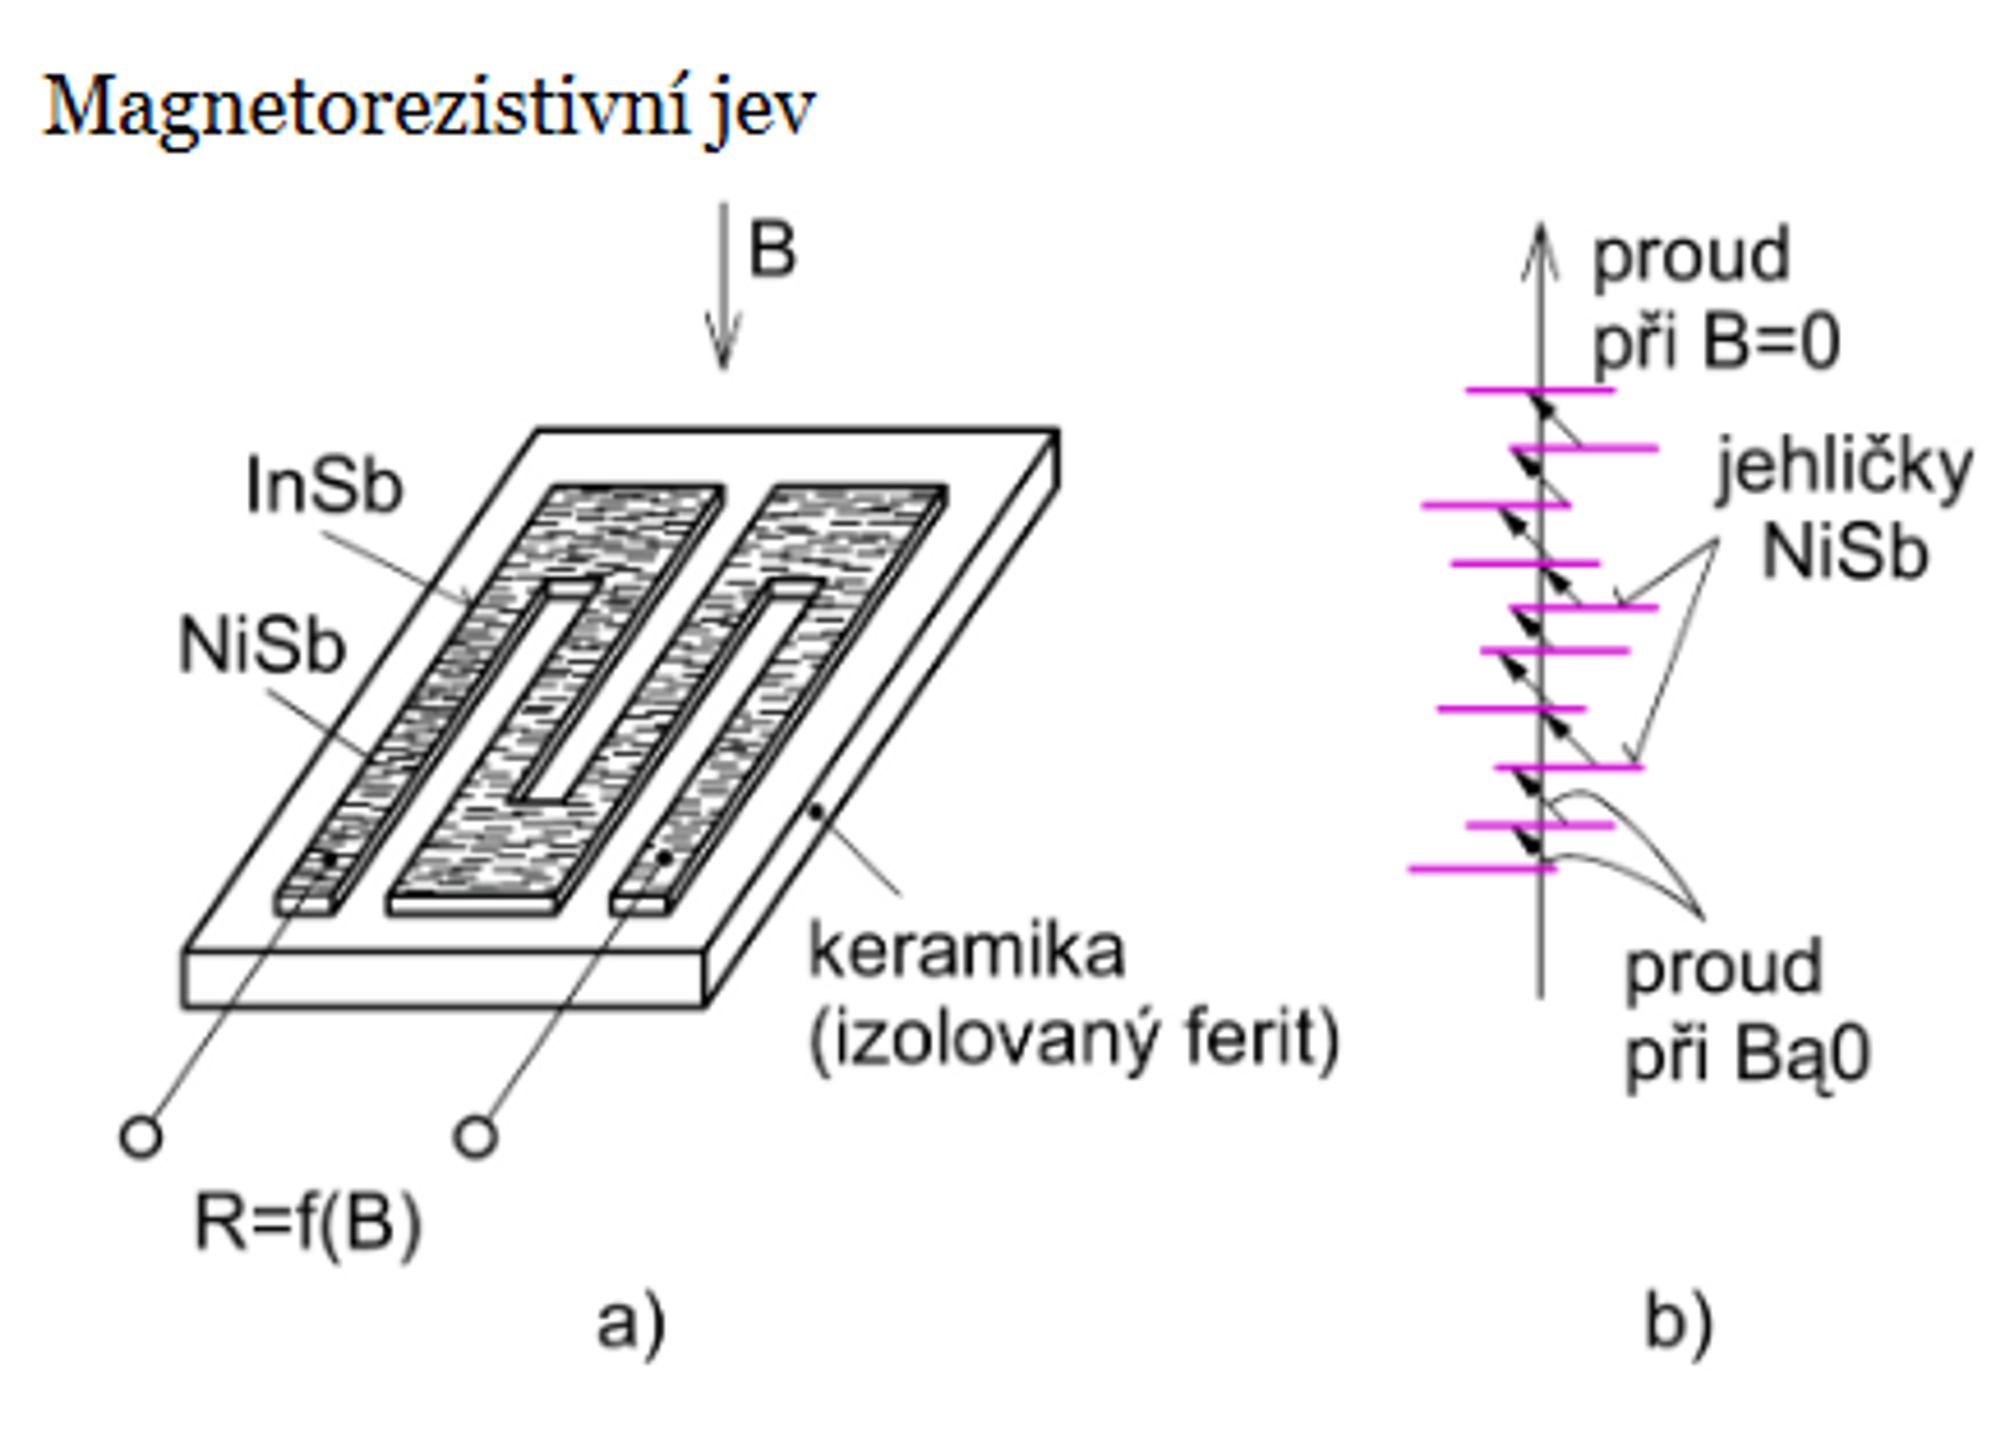
\includegraphics[scale = 0.1]{img/MagnetoRez.png}
\end{figure}

Častěji se využívá anizotropní magnetorezistivní jev - není stejný ve všech geometrických směrech. Aniztropní materiál má v sobě nějakou nesymetričnost. Tato je v našem případě to že mění svůj odpor různě podle toho v jakém směru na něj působí magnetické pole. Například permaloy.
Princip anizotropní: vrstvou necháváme procházet proud, když na vrsvu bude působit vnější magnetické pole a budeme měnit úhel jeho působení vůči úhlu proudu procházejícímu destičku, tak budeme měnit výsledný odpor. Největší odpor při kolmém působení, neprojeví se když je souběžné se směrem proudu.\\
Poměrně lineární, stabilní a opakovatelná.\\
\begin{figure}[h!]
    \centering
    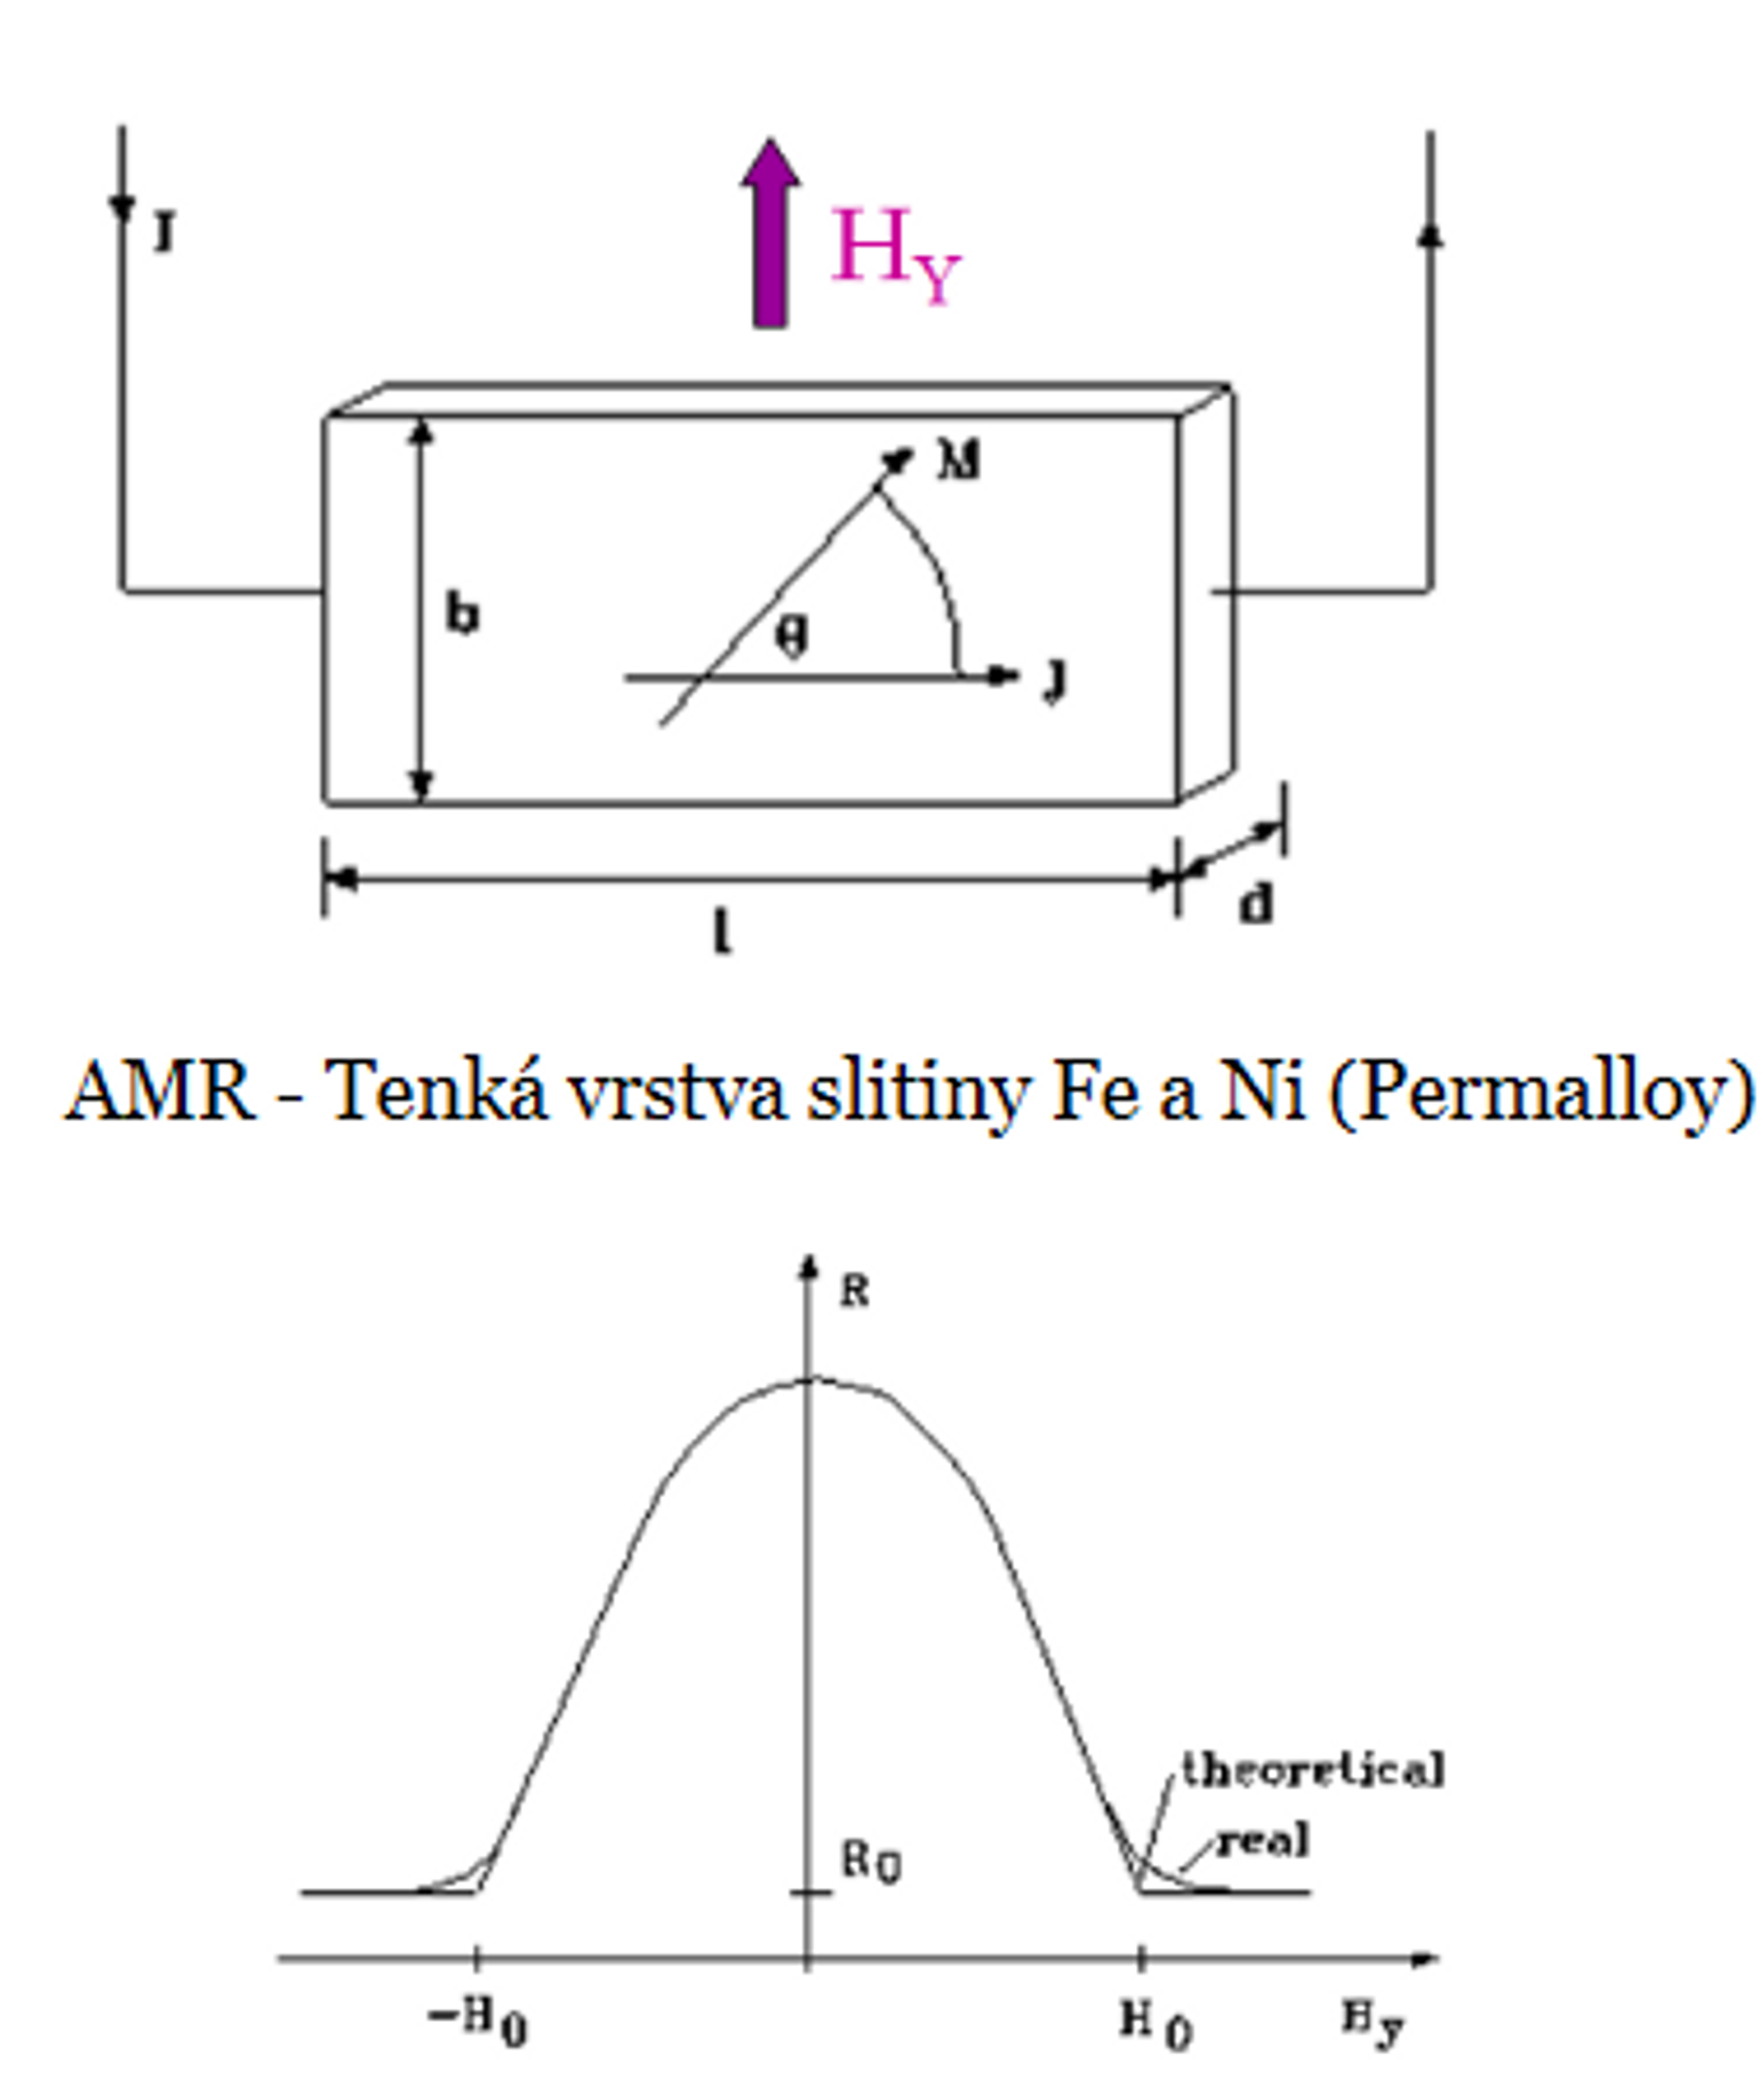
\includegraphics[scale = 0.1]{img/AnizoMag.png}
\end{figure}
Obří magnetorezistence - GMR.\\
Velký závislost na teplotě, nelineárnější než AMR.\\
Tunelové magnetorezistence - TMR.\\
Elektrony tunelují skrze vrstvy - kvantová fyzika hard.\\
\subsubsection*{AMR}
Zapojuje se do Whitsonova můstku ze 4 magnetorezistorů.\\
Pokud není MP přítomno, můstek je vyvážený a měřené napětí je nulové, když bude MP působit můstek se rozváží a my naměříme napětí.\\
Vždy se u 2 magnetorezistorů odpor zvětší a u 2 zmenší.\\

\begin{figure}[h!]
    \centering
    \begin{minipage}[b]{0.4\textwidth}
        \centering
        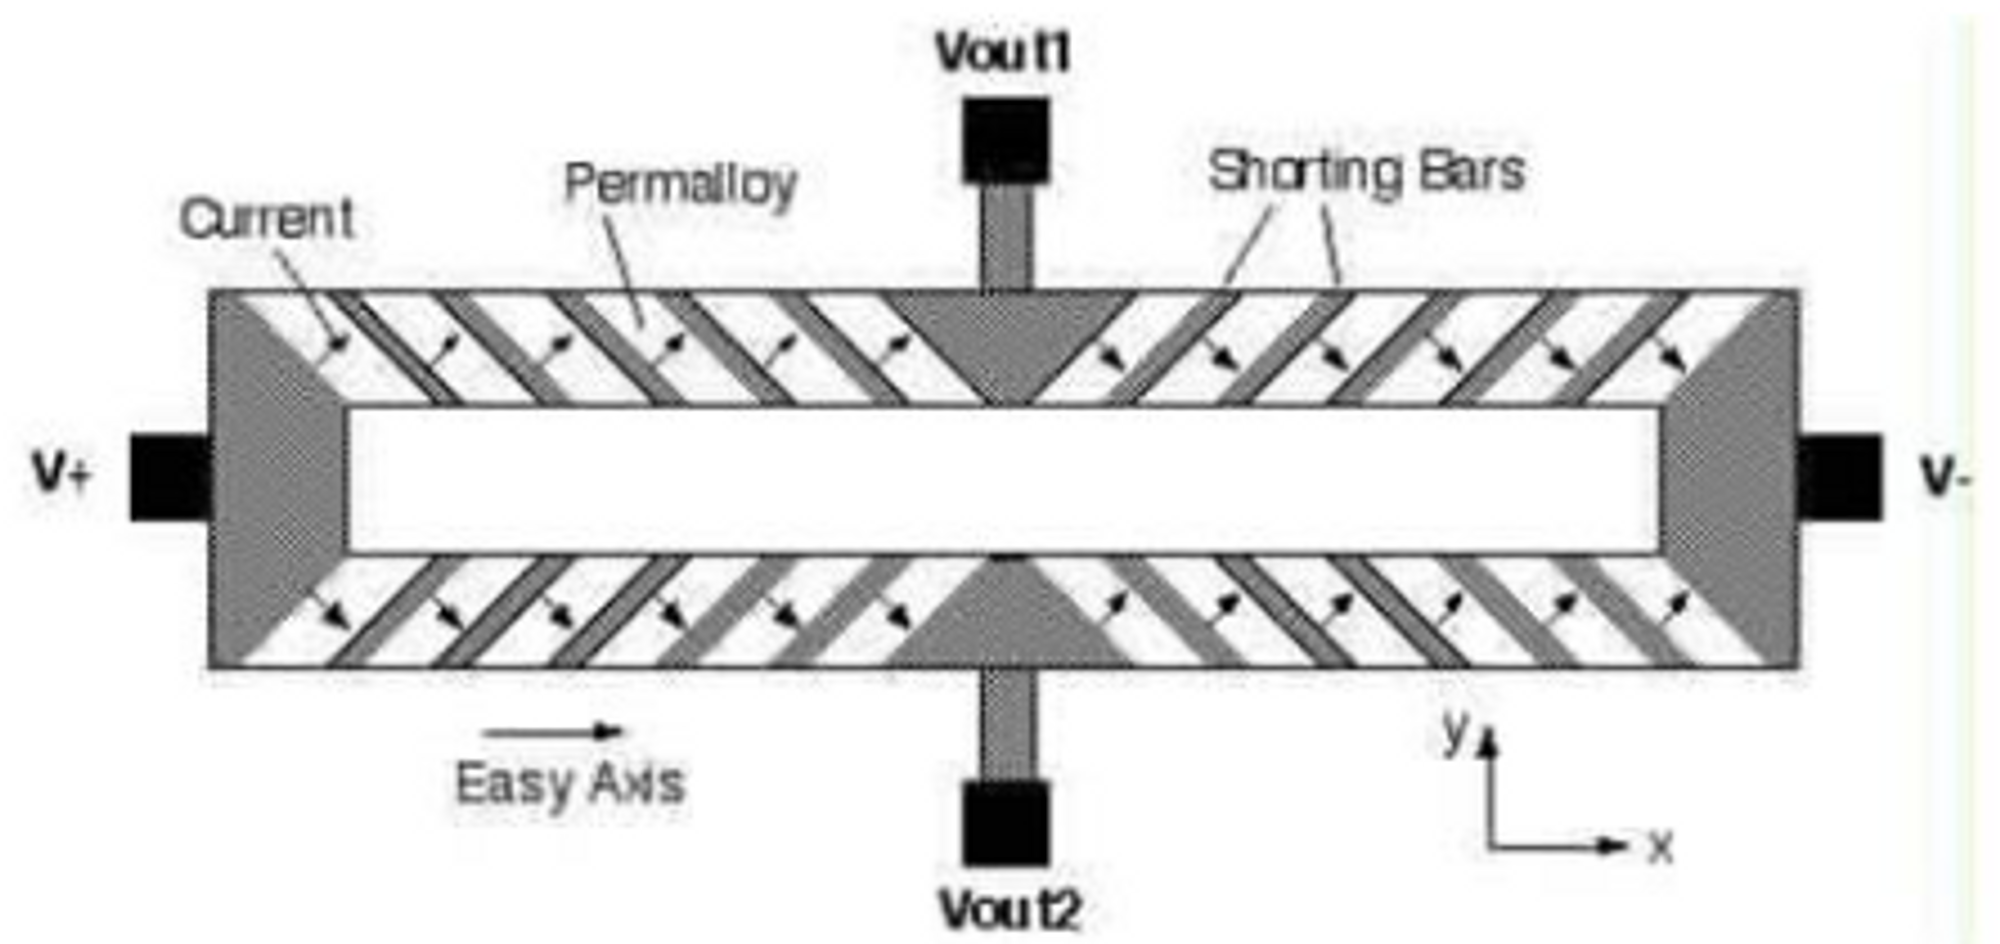
\includegraphics[width = \textwidth]{img/AMR1.png}
    \end{minipage}
    \hfill
    \begin{minipage}[b]{0.4\textwidth}
        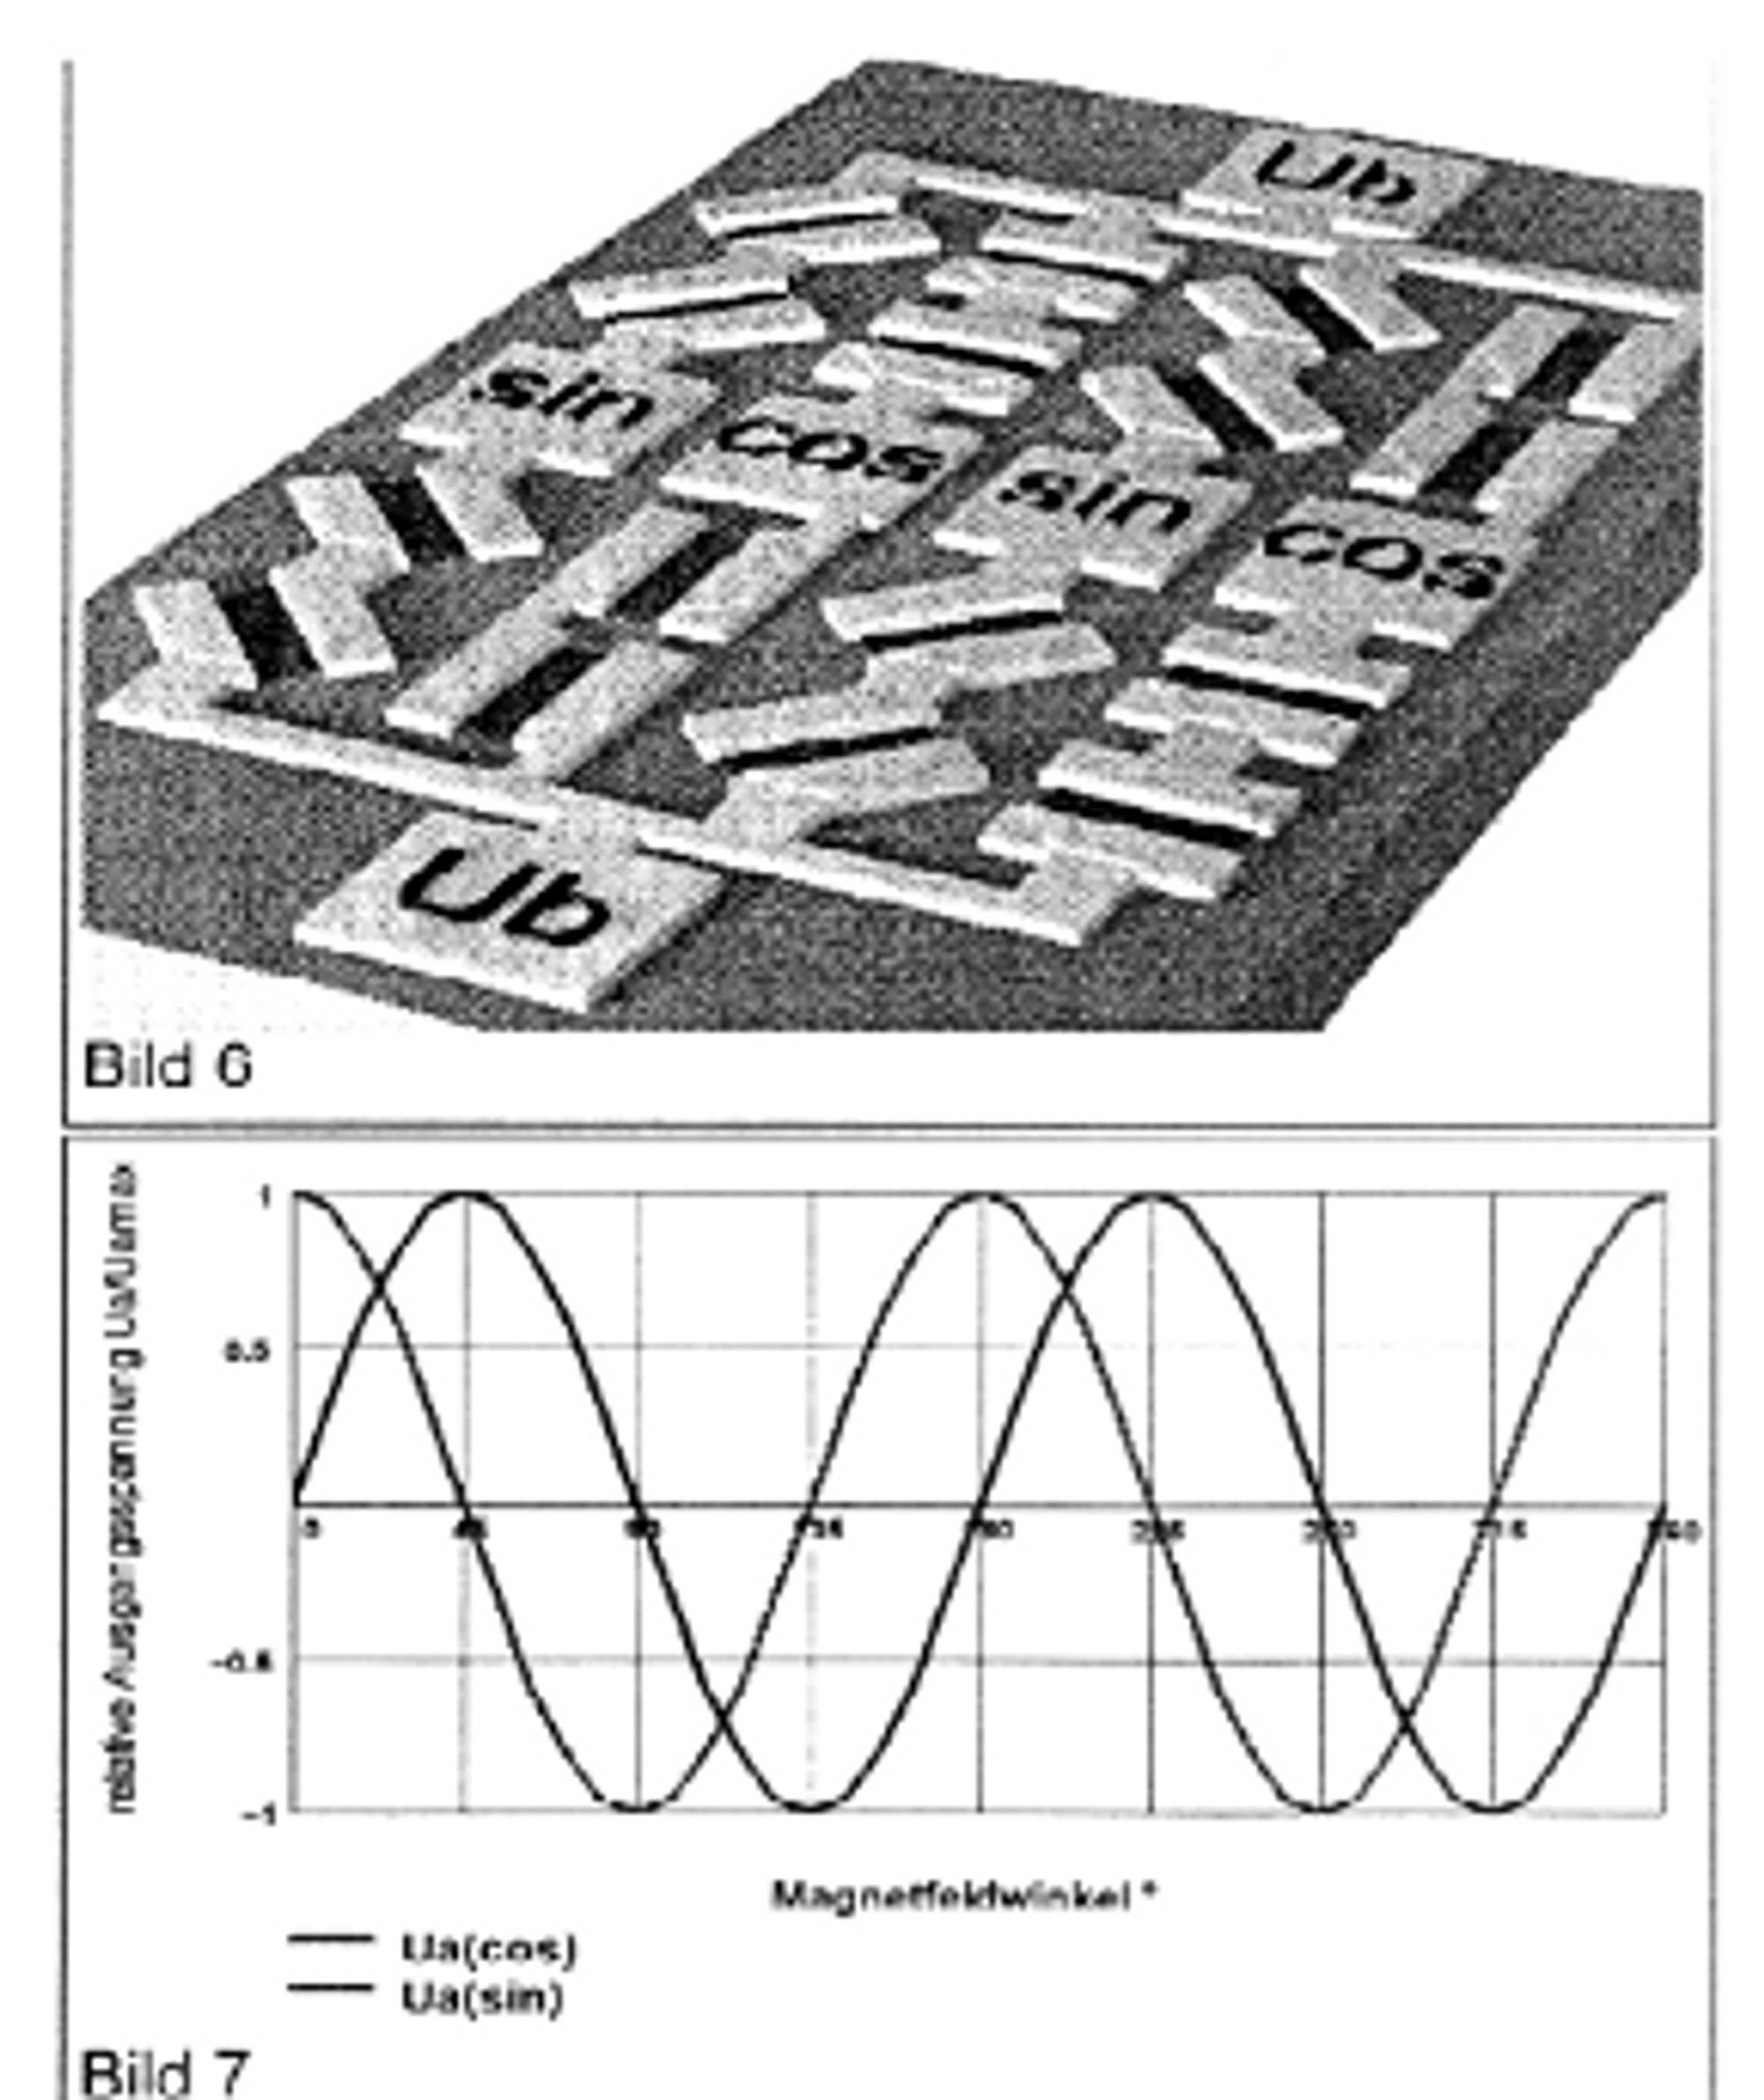
\includegraphics[width = \textwidth]{img/AMR2}
    \end{minipage}
\end{figure}

\subsubsection{Magnetostrikční snímače}
Využívá anizotropii, ale mechanickou a ne magnetickou.\\
Vyrobeny ze slitiny niklu, když je takový materiál vložen do magnetického pole, tak mění své rozměry. V jednom směru se rozměr zvětší a ve druhém zmenší.\\
Trubka z magnetostrikčního materiálu, trubkou je protažen vodič. Když se do vodiče přivede elektrický proud, tím se kolem něj vytvoří magnetické pole. Kolem vodiče je umístěn permanentní magnet tvořící své vlastní magnetické pole. V místě kde se tato pole setkají se pole superponují a mění svoji orientaci magnetické indukce/intenzity. V místě kde se pole setkají bude materiál vystaven jinému vektoru magnetické intezity což vede ke změně rozměru trubky.\\
Místo stálého vedení proudu posíláme proudový impulz, díky kterému vznikne škubnutí trubky. Měříme časový interval mezi vysláním proudového impulzu a příchodem mechanické vlny. Měříme nejčastěji piezoelektrickým materiálem. Tím změříme polohu permanentního magnetu.\\
Snímač lineárního posunutí. Rozsah i několika metrů, vysoká přesnost(mm).\\
Problémem je vliv teploty. Řeší se detekcí i poměrem časů příchodů mechanických vln, jedné přímé a jedné odražené od konce trubky.\\

\begin{figure}[h!]
    \centering
    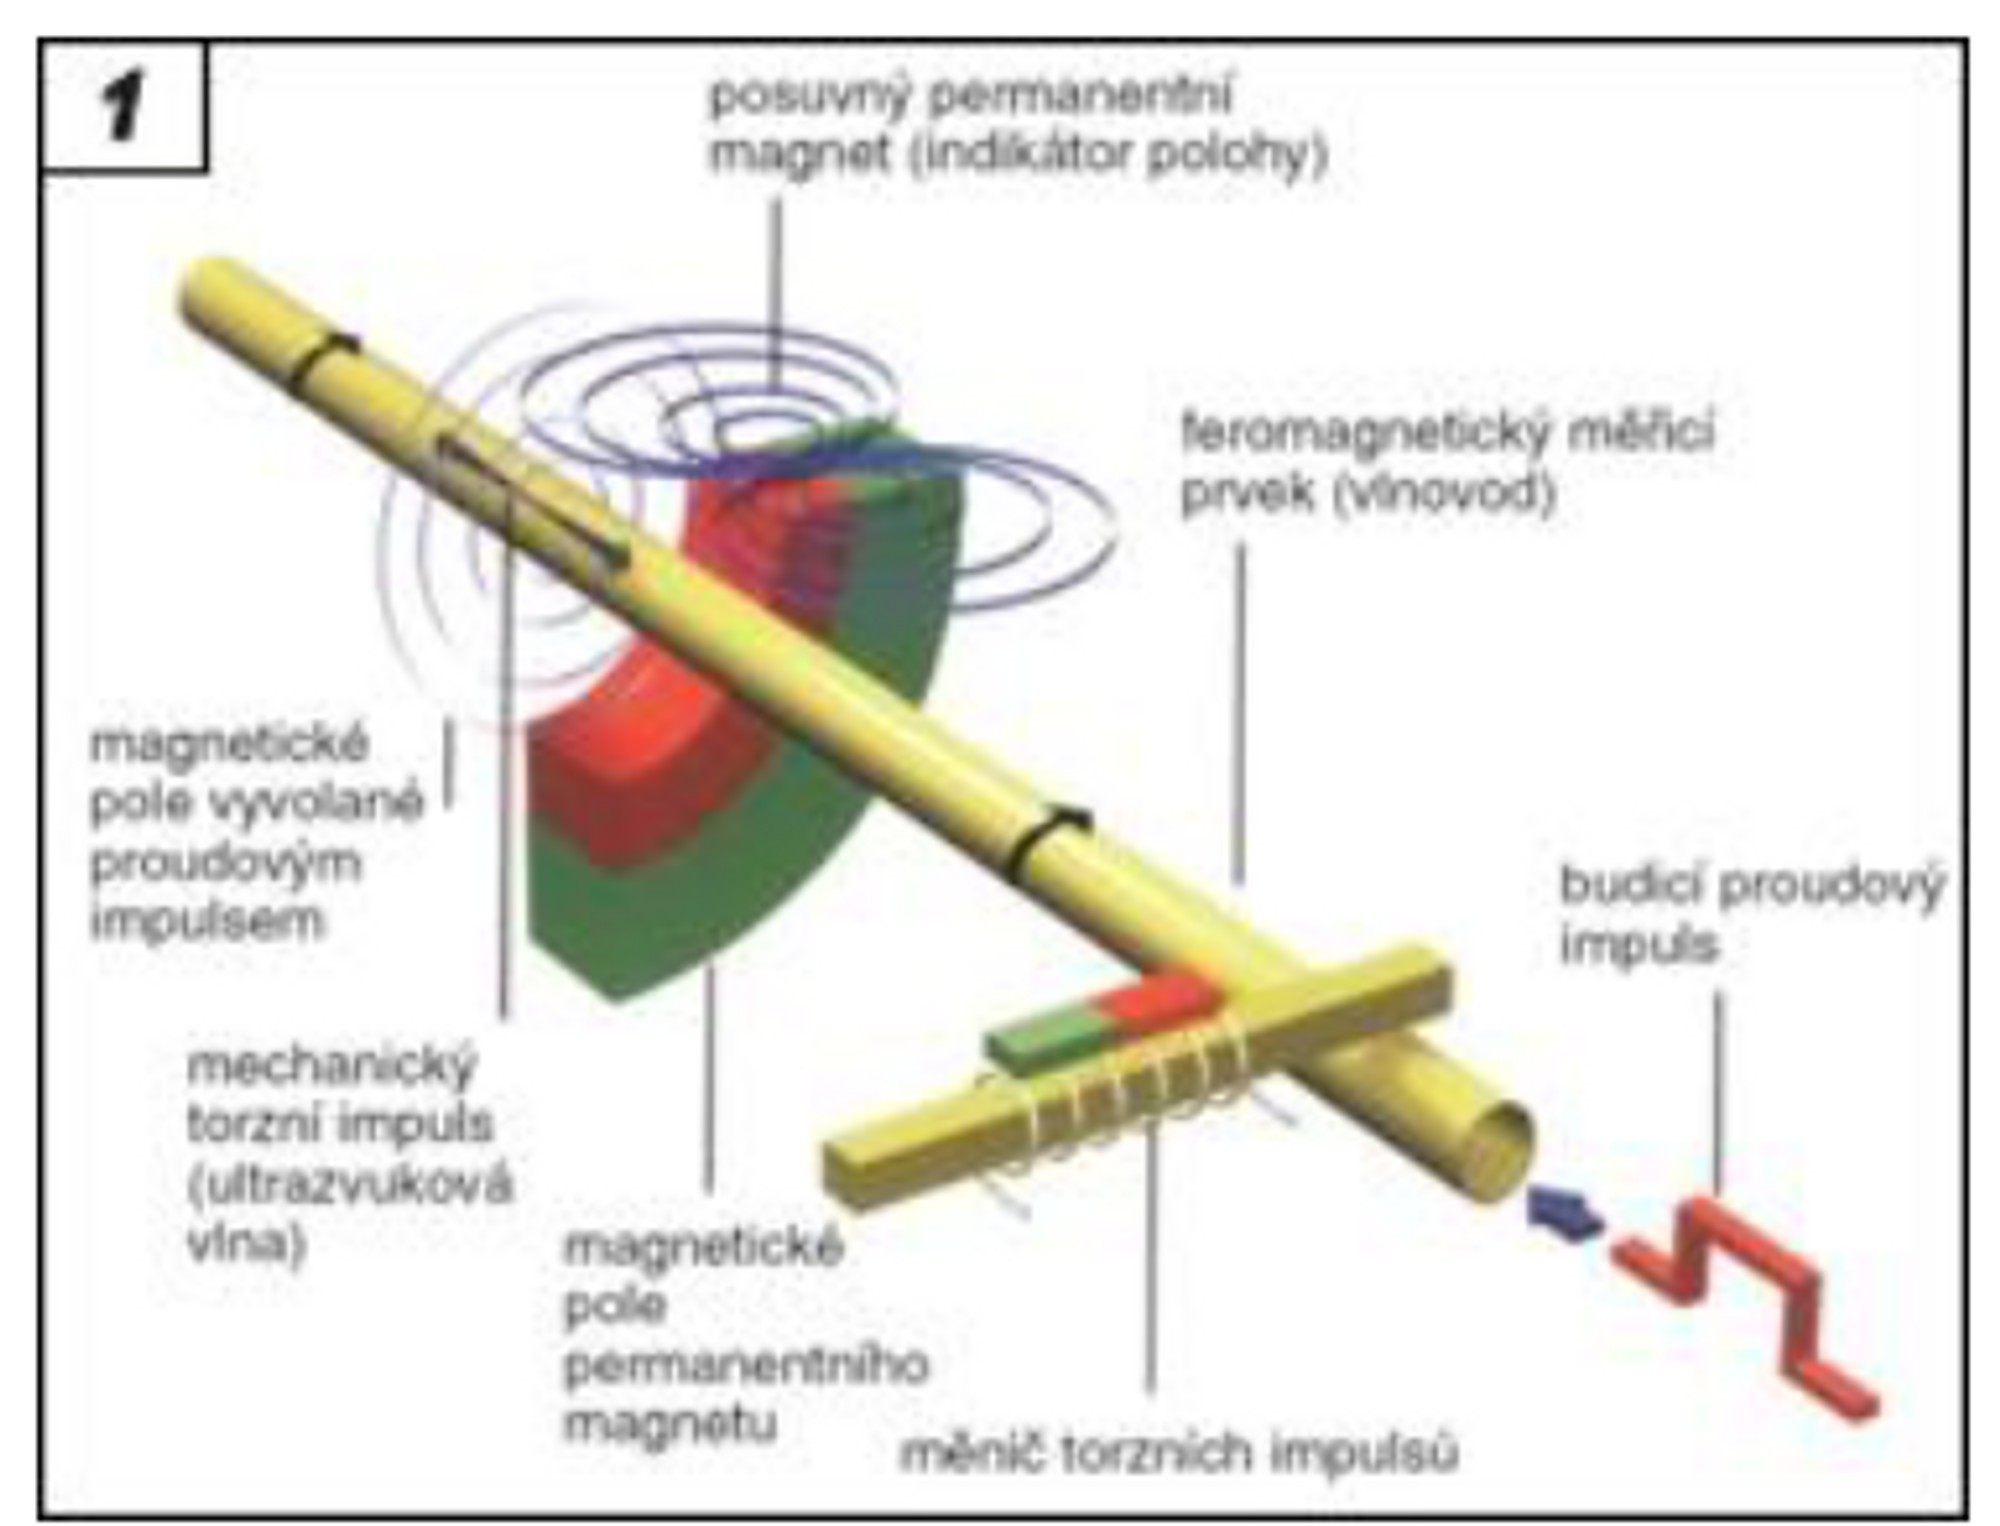
\includegraphics[scale = 0.1]{img/Magnetostrik.png}
\end{figure}
\subsection{Ultrazvukové snímače polohy}
Stejný princip jako doba letu u optických, tím že je rychlost menší, což se lépe měří a jsou jednodušší na zpracování, ale jsou méně přesné.\\
Mechanické vlnění, které se šíří nějakou rychlostí, závisí na materiálech, největší vliv teplota, ovlivňuje konstanty materiálů.\\
Vzdálenost minimálně taková, aby se signál nevracel v dobu, kdy se ještě vysílá a maximální, aby se něco vrátilo zpět.\\
Přídavná měřidla pro korekci okolních vlivů, například teploty.\\
Je tvořen piezoelektrickým měničem.\\
Měření doby letu pro větší vzdálenosti 30cm+, pro kratší se měří rozdíl fáze.\\
\begin{figure}[h!]
    \centering
    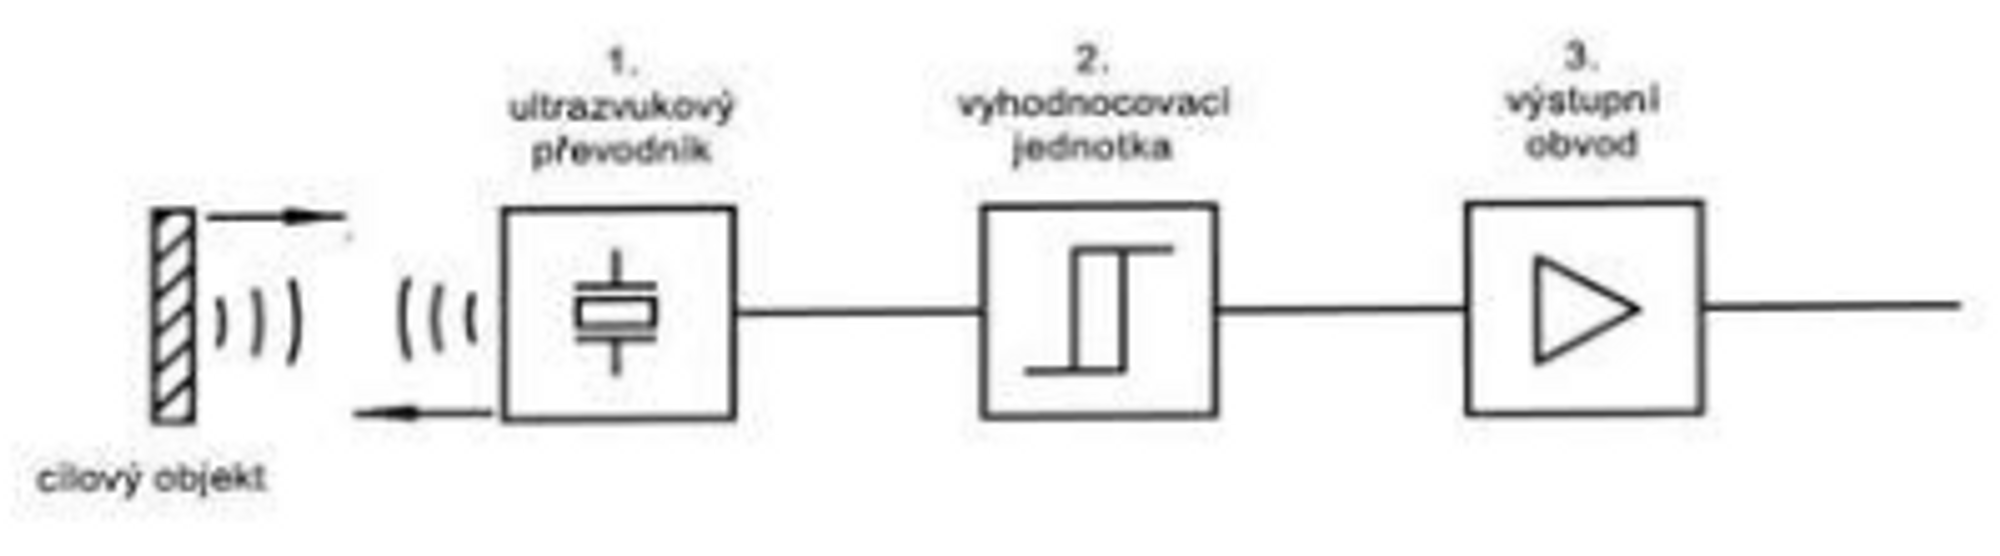
\includegraphics[scale = 0.1]{img/ultrazvPol.png}
\end{figure}

\subsection{Srovnání}
\begin{figure}[h!]
    \centering
    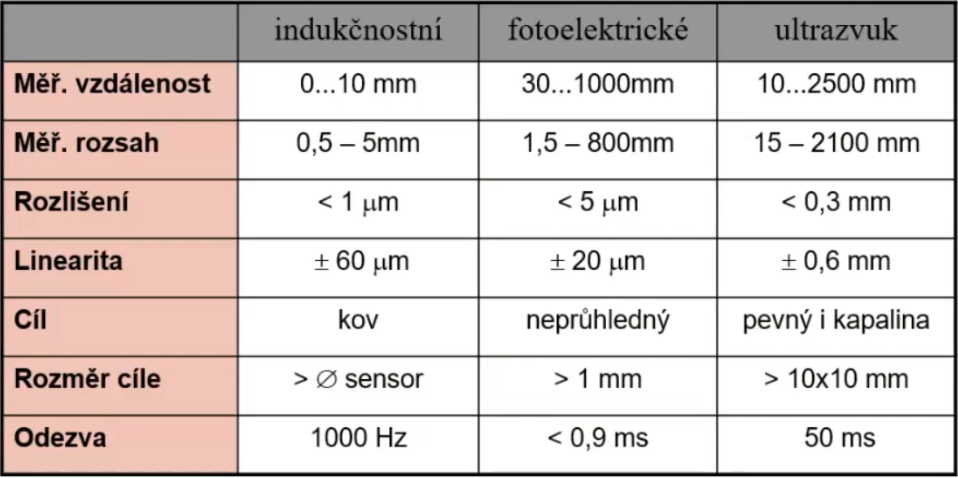
\includegraphics[scale = 0.3]{img/srovnaniPoloh.png}
\end{figure}

\section{Měření vibrací, rychlosti, zrychlení, akcelerometry, snímače úhlové rychlosti}
Kmitavým pohybem se rozumí časová změna polohy vybraného bodu na objektu vzhledem ke vztažnému (referenčnímu) bodu. K přímému měření okamžitých hodnot polohy je tedy obecně možné použít senzory polohy - v tomto případě jde o relativní senzory kmitavého pohybu, jelikož je určována poloha relativně k pevnému vztažnému bodu.

\subsubsection*{Rozdělení}
\begin{itemize}
    \item Dle typu měřené veličiny \begin{itemize}
              \item Lineární \begin{itemize}
                        \item Rychlost - měřič rychlosti
                        \item Zrychlení - akcelerometr
                    \end{itemize}
              \item Rotační \begin{itemize}
                        \item Odklon od roviny - inklinometr
                        \item Otáčky - snímač otáček, tachometr, otáčkoměr
                        \item Úhlová rychlost - gyroskop
                    \end{itemize}
              \item Vibrace (kmity kolem rovnovážné polohy) \begin{itemize}
                        \item Výchylka, rychlost, zrychlení - měřič vibrací, akcelerometr
                    \end{itemize}
          \end{itemize}
    \item Dle fyzikálního principu \begin{itemize}
              \item Piezoelektrické
              \item Kapacitní
              \item Indukční, elektrodynamické
              \item Optické (LIDAR, interferometry, kamera)
              \item Speciální - magnetické, tepelné
          \end{itemize}
\end{itemize}

\subsubsection*{Snímače vibrací}
\begin{itemize}
    \item Vibrace - kmitavý pohyb, můžeme použít libovolný snímač polohy, výsledkem je relativní snímač vibrací
    \item Výchylka - vzdálenost vibrujícího tělesa od referenčního bodu
    \item Rychlost - rychlost, kterou se těleso pohybuje
    \item Zrychlení - zrychlení, kterým se těleso pohybuje
\end{itemize}

Pokud neexistuje pevný referenční bod, potřebujeme absolutní snímač vibrací. Pevný referenční bod se vytvoří uměle pomocí setrvačné hmoty uvnitř snímače, poté se měří silové účinky setrvačné hmoty pomocí relativního snímače polohy (kapacitní, indukční, indukčnostní) nebo snímače mechanického napětí (odporový tenzometr, piezoelektrický krystal,\dots)
Absolutní snímač vibrací lze využít pro inerciální navigaci - zvýšení přesnosti a stability dosaženo elektromechanickou zpětnou vazbou.

\subsubsection*{Absolutní snímač vibrací}
\begin{itemize}
    \item Používá se v případě neexistujícího pevného referenčního bodu.
    \item Podstatou mech. kmit. soustava o hmotnosti m, pružinou o tuhosti k a tlumič s viskózním tlumením b (často zanedbáváme, protože je vůči objektu malé)
    \item Pomyslný bod A leží na měřeném objektu.
\end{itemize}

\begin{figure}[h]
    \centering
    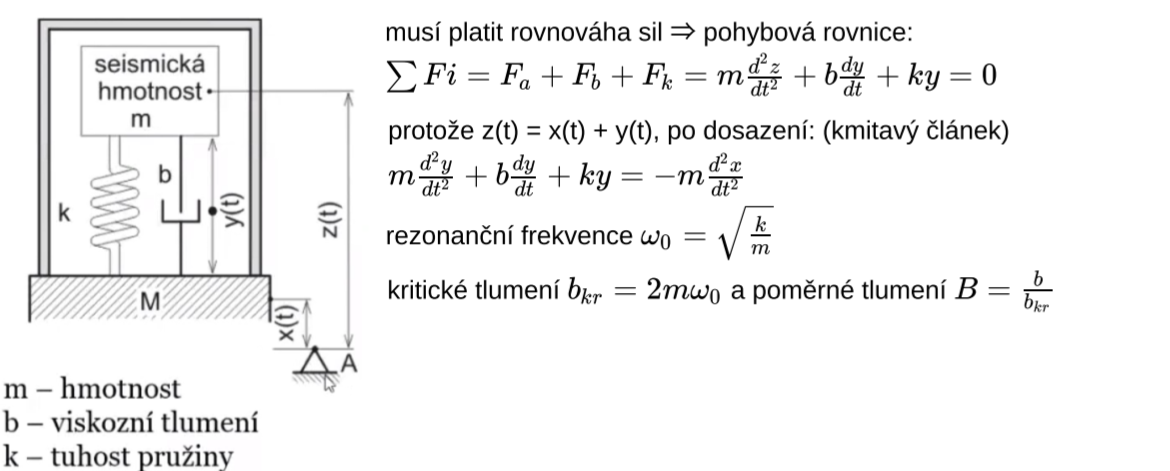
\includegraphics[scale = 0.5]{img/AbsVib.png}
\end{figure}

\begin{figure}[h]
    \centering
    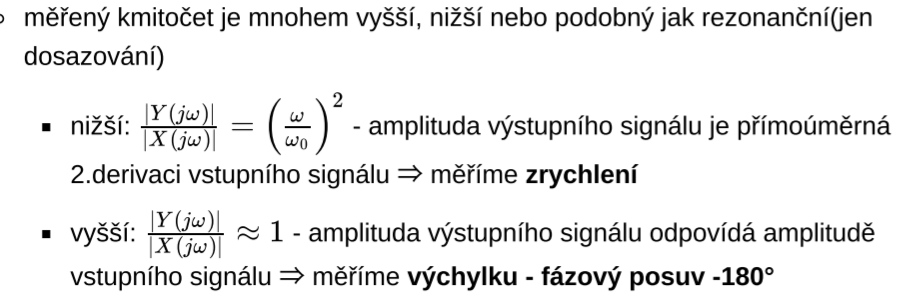
\includegraphics[scale = 0.5]{img/AbsVib1.png}
\end{figure}

\newpage

\subsection*{Elektrodynamický snímač vibrací - indukční}
\begin{itemize}
    \item Pracuje v nadrezonanční oblasti -> měření výchylky
    \item Konstrukčně uspořádán jako reproduktor - pracuje v inverzním režimu
    \item Seismickou hmnotnost zde tvoří měřící cívka a cívka tlumení
    \item Tlumení - vířivé proudy indukované v tlumící cívce
\end{itemize}

\begin{figure}[h]
    \centering
    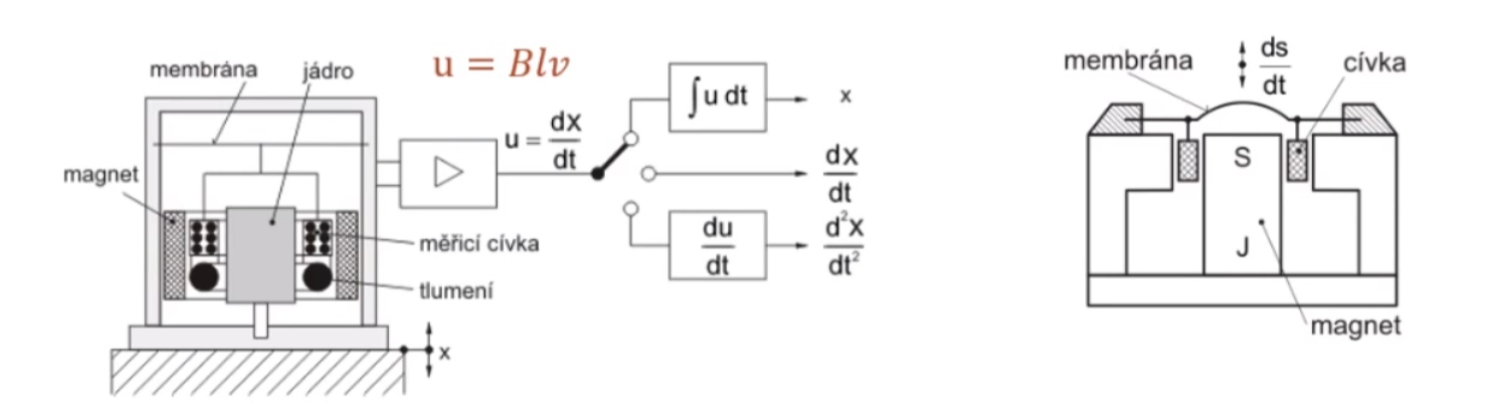
\includegraphics[scale = 0.4]{img/elektrodynVIB.png}
\end{figure}

\begin{itemize}
    \item Reproduktor v inv. režimu(obr. vpravo) - Permanentní magnet s pólovými nástavci. Vzniká Homogenní magnetické pole ve štěrbině, kde se pohybuje cívka (šrafovaně), pohybuje se nahoru a dolů v poli permanentního magnetu. Kvůli lorenzově síle bude cívka vytlačována nebo vtahována do magnetického pole a membrána se pak hýbe - mechanické vlnění -> zvuk
    \item obr. vlevo - Hýbeme membránou (setrvačnou hmotou) připojenou k měřenému povrchu, dojde k vzájemnému pohybu megnetu vůči setrvačné hmotě - do cívky se indukuje napětí úměrné rychlosti pohybující se cívky v magnetickém poli.
\end{itemize}

$u = B*l*v$
\begin{itemize}
    \item l - délka cívky
    \item B - magnetická indukce v mezeře
    \item v - rychlost magnetického pole
\end{itemize}

\subsubsection*{Použití}
\begin{itemize}
    \item V nadrezonanční oblasti - řežim měření výchylky - výstup úměrný rychlosti pohybu cívky v mag. poli
    \item Vhodné pro nižší kmitočky do 100 Hz
    \item Geofony - pro měření vibrací země - využití velké setrvační hmoty
    \item Extrémní citlivost - detekce ponorek
\end{itemize}

\subsection*{Piezoelektrický snímač vibrací}
\begin{itemize}
    \item Využívá piezoelektrického jevu \begin{itemize}
              \item Jednoduše: Na piezoelektrický materiál je vyvíjeno mechanické napětí, tím se mění jeho tvar nebo objem, to vede k vytvoření elektrického náboje.
              \item Složitě: Na piezoelektrický materiál, dielektrikum, který je mechanicky namáhán, dojde ke změně vnitřní polohy atomu v krystalové mřížce. Navenek se to projeví tak, že dojde k rozvážení vnitřní elektrické polarizace. Toto se projeví tak, že se materiál stane elektrický aktivní (předtím neutrální), objeví se na jeho povrchu náboj a v případě, že na toto dielektrikum přivedeme elektrody, můžeme na něm sledovat změnu náboje.
          \end{itemize}
    \item Pracují v podrezonanční oblasti
    \item Výchylka se měří tak, že se převede na mechanícké napětí
    \item Piezoelektrický materiál představuje pružnost/tuhost materiálu
\end{itemize}

\begin{figure}[h]
    \centering
    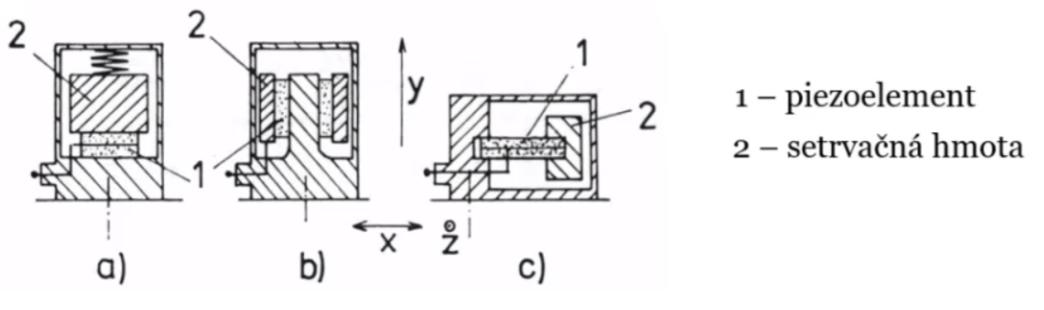
\includegraphics[scale = 0.40]{img/piezoVIB.png}
\end{figure}

\begin{figure}[h]
    \centering
    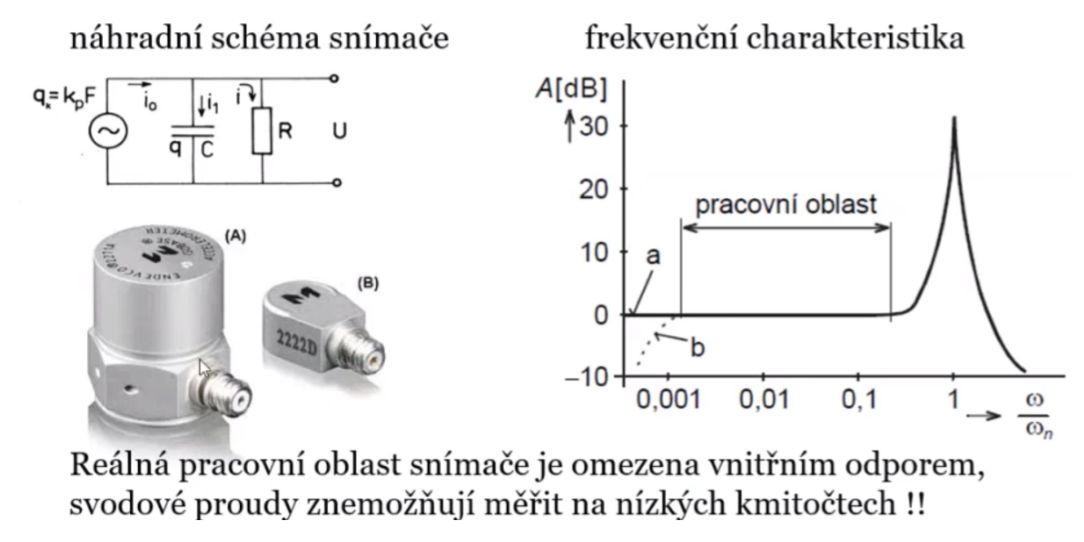
\includegraphics[scale = 0.50]{img/piezoVIB1.png}
\end{figure}

\begin{itemize}
    \item Pracovní oblast je dána frekvenční charakteristikou \begin{itemize}
              \item Na jedné straně požadavek, aby pracoval pod rezonanční oblastí
              \item Ze spoda je omezena - vychází ze schéma, náboj se generuje jenom při působívcí síle, což nabije kondenzítor, který neudrží do nekonečna -> na nízkých kmitočtech se nestíhá kondenzátor dobíjet
          \end{itemize}
\end{itemize}

\subsubsection*{Snímač vibrací s vetknutým nosníkem}
\begin{itemize}
    \item Typické pro MEMS snímače
    \item Setrvačná hmota, ale neměří se mechanické účinky, měří se změna polohy setrvačné hmoty vůči obalu - pevným elektrodám.
\end{itemize}

\begin{figure}[h]
    \centering
    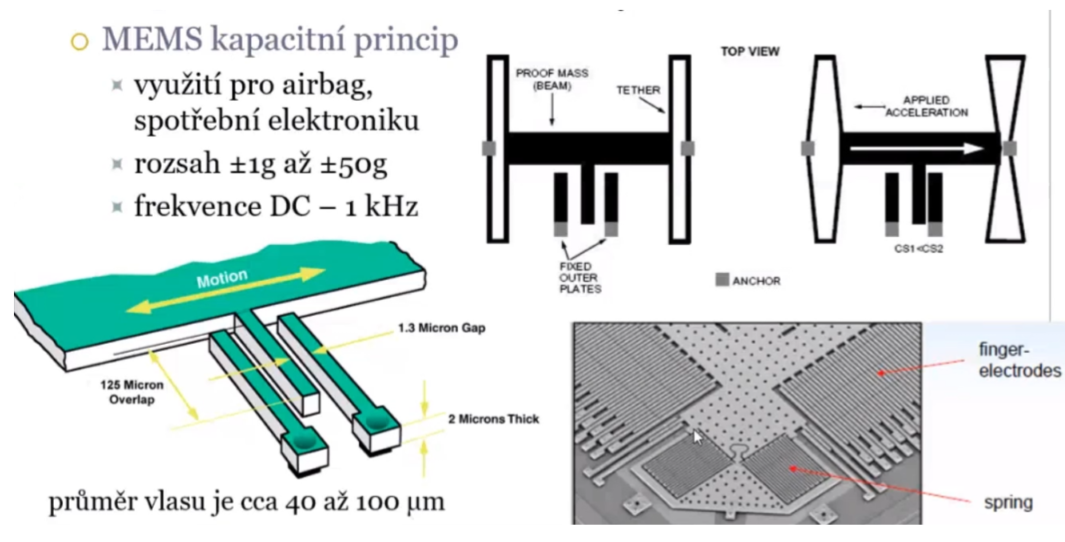
\includegraphics[scale = 0.50]{img/MEMSVIB.png}
\end{figure}

\begin{itemize}
    \item Měří se změna střední elektrody vůči krajním
    \item Pracuje v podrezonanční oblasti -> snímač zrychlení - výchylka odpovídá zrychlení
    \item Zespoda není omezen, z vrchu dostatečnou citlivostí
    \item Vyhodnocuje se výchylka nosníku deformovaného setrvačnou hmotou pomocí diferenčního kapacitního snímače (další možností je měřit mech. napětí v nosníku tenzometry)
\end{itemize}

\subsubsection*{Tepelný akcelerometr}
\begin{itemize}
    \item Setrvačná hmota je zahřátý plyn, měří se rozdíl teplot
    \item Je to tenká membrána, která má uprostřed topné tělísko, kterým vyhřívá okolí
    \item Ohřev způsobí rozložení teploty tím, jak se budeme vzdalovat od topného tělíska ke krajům -> klesá teplota
    \item Pokud snímač naklopíme, teplý plyn nejde nahoru, protože je to setrvačná hmota, zůstane tam, kde byl a pod něj se v podstatě podsune snímač teploty, který měří rozložení teploty v okolí tělesa
    \item Vyhodnocuje se změna polohy, podle polohy topného tělíska
    \item Měření náklonu
    \item Nemá rezonanční kmitočet
\end{itemize}

\begin{figure}[h]
    \centering
    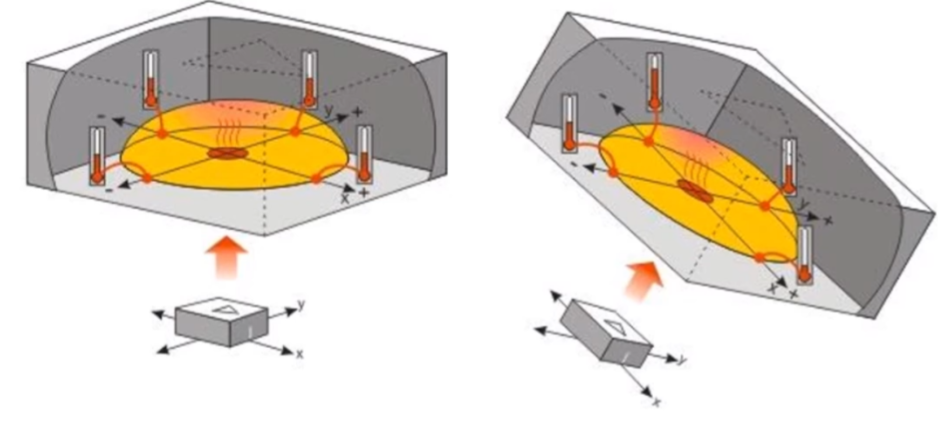
\includegraphics[scale = 0.50]{img/teplovib.png}
\end{figure}

\subsubsection*{Servoakcelerometr}
\begin{itemize}
    \item Vysoce přesné a stabilní => drahé
    \item Pro navigační účely
    \item Pro určení polohy nutná dvojí integrace => vysoké požadavky na stabilitu nuly
    \item Využíváme zpětnou vazbu na stabilitu nuly
    \item Čerevené kolečko - setrvačná hmota zavěšená na nosníáku, při pohybu se začne vychylovat.
\end{itemize}

\begin{figure}[h]
    \centering
    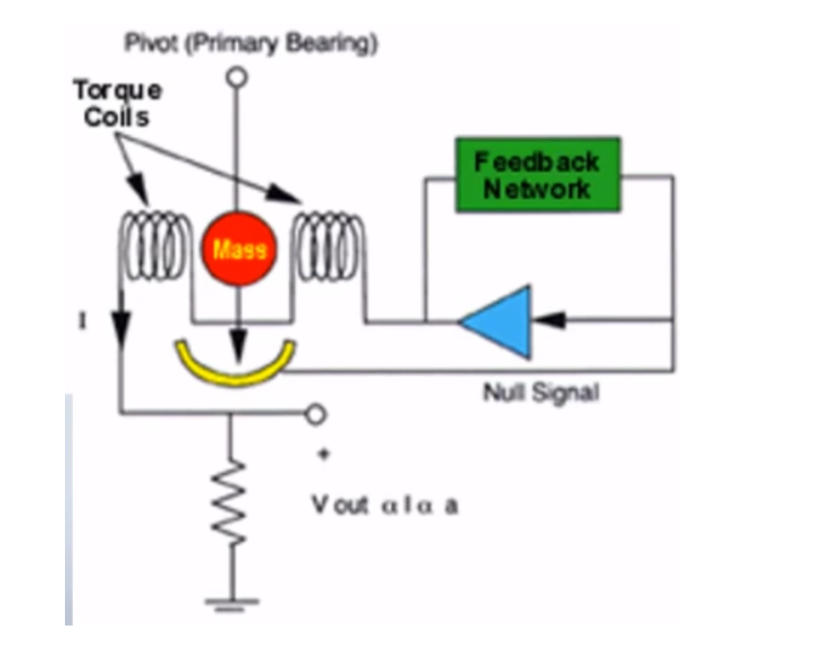
\includegraphics[scale = 0.50]{img/servoakVIB.png}
\end{figure}

\begin{itemize}
    \item Indikátor vyrobí nenulový singál, který je zesílen zesilovačem
    \item To žluté je snímač polohy
    \item Setrvačná hmota je kovová a lorenzova síle z cívek, kterýma protéká proud působí na setrvačnou hmotu
    \item Výstupní veličina je proud, který pak putuje do cívek, pomocí který setrvačnou sílu dáváme do nulové polohy
\end{itemize}

\subsection*{Snímače otáček}
\subsubsection*{Tachodynamo}
\begin{itemize}
    \item analogový snímač úhlové rychlosti
    \item Komutátorový motor v inverzním režimu
    \item Otáčí se motorem a měří se indukované výstupní napětí
    \item Uzavřený magnetický obvod, ve kterém je vzduchová mezera a v té se otáčí cívka. Jak se mění poloha cívky, tak se mění magnetický tok (cívka svisle = kolmo na siločáry = největší tok).
    \item Komutátory na začátku a na konci cívky - dochází k přepínání polarity.
    \item Přímo dává napětí, které je úměrné otáčkám
    \item Změní-li se směr otáčení - změní se polarita výstupního napětí
\end{itemize}

\begin{figure}[h]
    \centering
    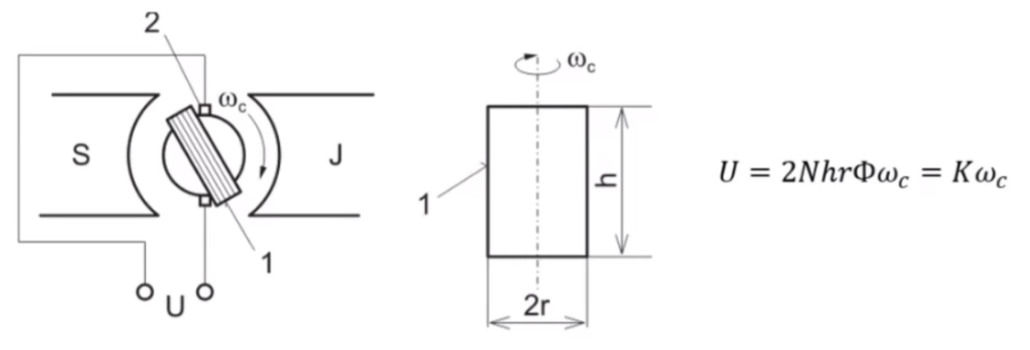
\includegraphics[scale = 0.50]{img/TachoRYCH.png}
\end{figure}

\subsubsection*{Impulzní snímače otáček}
\begin{itemize}
    \item Nespojité
    \item Detekuje se poloha značky - měří se počet značek za čas, časový interval mezi značkami
\end{itemize}

\begin{figure}[h]
    \centering
    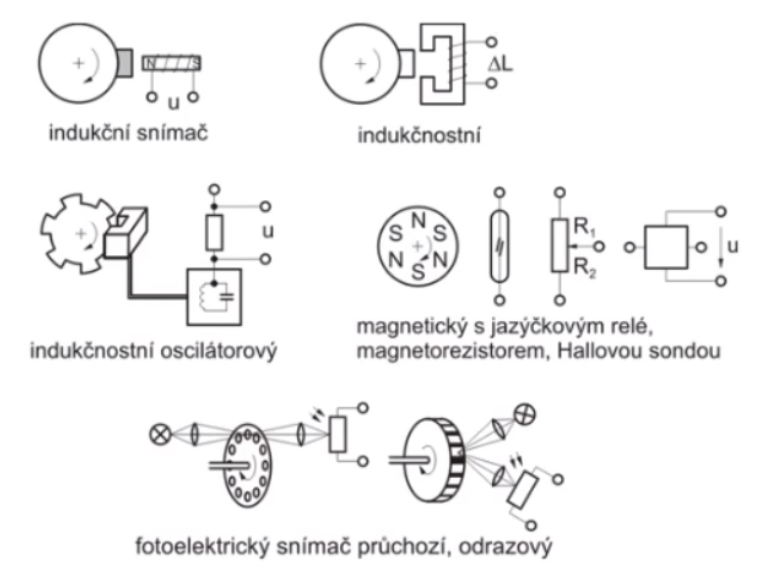
\includegraphics[scale = 0.50]{img/impulzRYCH.png}
\end{figure}

\begin{itemize}
    \item Indukční - nepotřebuje napájení, nedokáže indukovat malé Otáčky
    \item Indukčnostní - mění se indukčnost cívky - když zub najede mezi pólové nástavce, tak se zvětší indukčnost
    \item Oscilátorový - Jak se mění indukčnost, tak se mění v rezonančním rozsahu i rezonanční kmitočet - pak se měří impedance rezonančního obvodu
    \item Relé - Pomocí hallovy sondy, detekce otáčení kol
    \item Fotoelektrický - Nedokážeme u něj poznat směr
\end{itemize}

\subsection*{Snímače úhlové rychlosti}
\begin{itemize}
    \item Gyroskop - absolutní snímač úhlové rychlosti
    \item Mechanické
    \item S využitím Coriolisova jevu (MEMS) - 99 \% toto využívá \begin{itemize}
              \item Podle pohybu setrvačné hmoty - rotační, vibrační
              \item Podle způsobu buzení - elektromagnetické, piezoelektrické, elektrostatické
              \item Podle způsobu vyhodnocení - piezoelektrické, kapacitní, tunelový jev, SAW (povrcnová akustická vlna)
          \end{itemize}
    \item optické s využitím Sagnacova jevu - top shit \begin{itemize}
              \item FOG - fiber optic gyroscope - optická trasa vedená ve vlákně
              \item RLG - ring laser gyroscope - dutina laseru přímo zdroj laseru
          \end{itemize}
\end{itemize}

\subsubsection*{Mechanický gyroskop}
\begin{itemize}
    \item založen na rotující setrvačné hmotě s velkým momentem hybnosti
    \item Když ho roztočíme, má snahu zůstat ve své původní poloze, k vychýlení osy rotace potřebujem velkou sílu
    \item Úhel natočení vstupu je úměrný výstupnímu
    \item Příliš se nesetkáme
\end{itemize}

\begin{figure}[h]
    \centering
    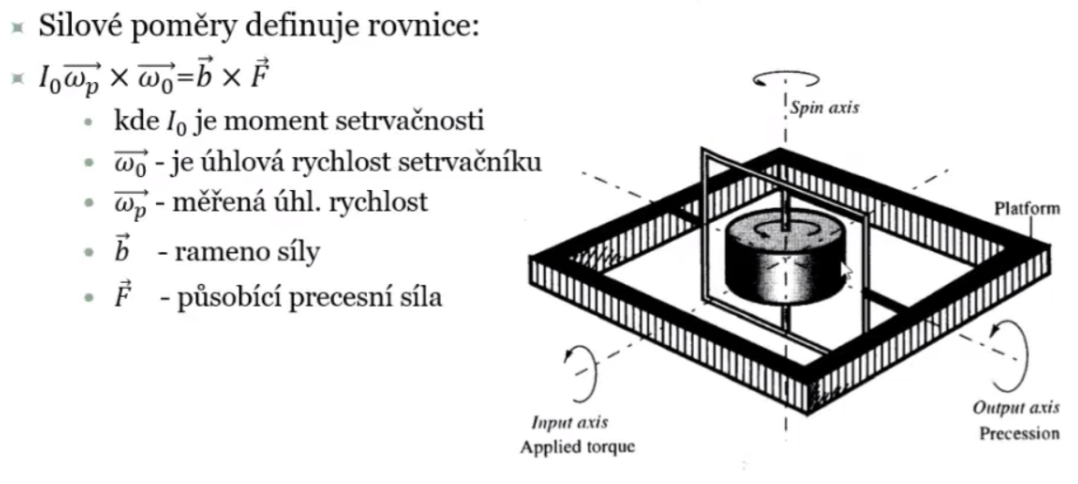
\includegraphics[scale = 0.50]{img/TyPicoMeTakBaviVypracovavatSnimace.png}
\end{figure}

\subsubsection*{MEMS gyroskop}
\begin{itemize}
    \item Měří se silový účinek Coriolisovy síly odpovídající úhlové rychlosti otáčení vibrujícího hmotného tělesa
    \item Coriolisova síla - virtuální síla, vzniká, když máme setrvačné těleso pohybující se v rotujícím neinerciálním systému \begin{itemize}
              \item Když se těleso nehýbe, nebo systém nerotuje, síle je nulová
              \item Když su na kolotoči a hodím míč dopředu, tak zahne - pro někoho mimo kolotoč to tak nevypadá
              \item V zeleném místě hážu míčem, rychlost je dána směrem pohybu (žluta čara), vektor úhlové rychlosti v ose rotace a kolmo na ty dva vektory je coriolisova síla
          \end{itemize}
\end{itemize}

\begin{figure}[h]
    \centering
    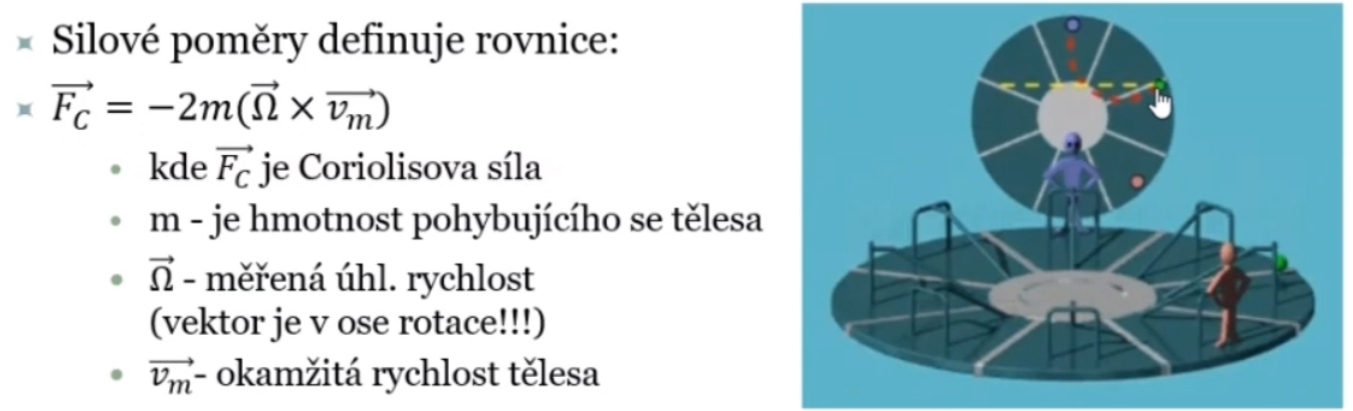
\includegraphics[scale = 0.40]{img/coriolis.png}
\end{figure}

\subsubsection*{MEMS gyroskop s lineárním (rotačním) rezonátorem}
\begin{itemize}
    \item Coriolisova síla způsobí výchylku vibrující setrvačné hmoty
    \item Otáčením rámu rozkmítáme krychlu aj do boku a pomocí kapacitních snímačů měříme změnu polohy krychle vůči obalu
    \item Když hýbem nahoru, tak coriolisiova síla působí směrem doleva
    \item Potřebná citlivost je mega velká, coriolisova síle je malá
\end{itemize}

\begin{figure}[h]
    \centering
    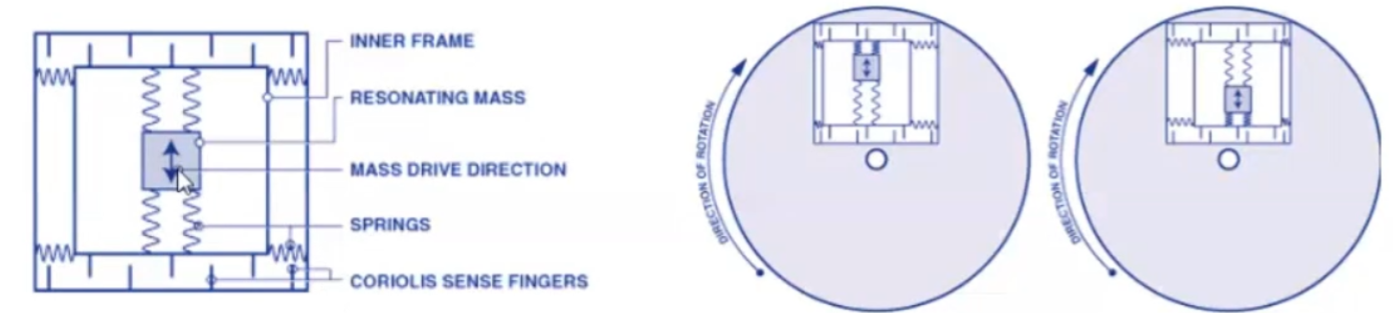
\includegraphics[scale = 0.40]{img/coriool123.png}
\end{figure}

\subsubsection*{MEMS gyroskop s vibračním rezonátorem (tunning fork)}
\begin{itemize}
    \item Coriolisova síla způsobí periodickou výchylku vibrujících ramen rezonátoru, kmity se přenesou na spodní ramena, kde se to vyhodnotí - třeba kapacitně
    \item Vidličky se od sebe vzdalují a přibližují, a když se vidlička začne otáčet, tak se začne působit coriolisova síla, takže v ose y bude na každou vidličku působit síla opačným směrem - to se vyhodnocuje
\end{itemize}

\begin{figure}[h]
    \centering
    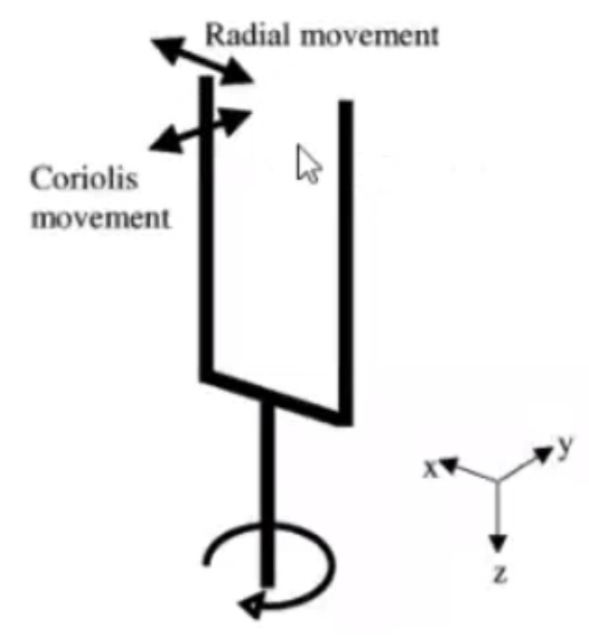
\includegraphics[scale = 0.40]{img/vidlicka.png}
\end{figure}

\subsubsection*{MEMS gyroskop s vibrujícím prstencem}
\begin{itemize}
    \item Coriolisova síla způsobí úhlové natočení kmitem a uzlů
    \item Když kroužíme na vrchní hraně kulaté skleničky mokrým prstem, tak vydává zvuky - vyvolá se tím rezonance skleničky, pod mikroskopem by šlo vidět, že mění svůj tvar.
    \item Do místa uzlů se dávahá snímače polohy - coriolisova síla je kolmá na vektor úhlové rychlosti a vektor rychlosti
\end{itemize}

\begin{figure}[h]
    \centering
    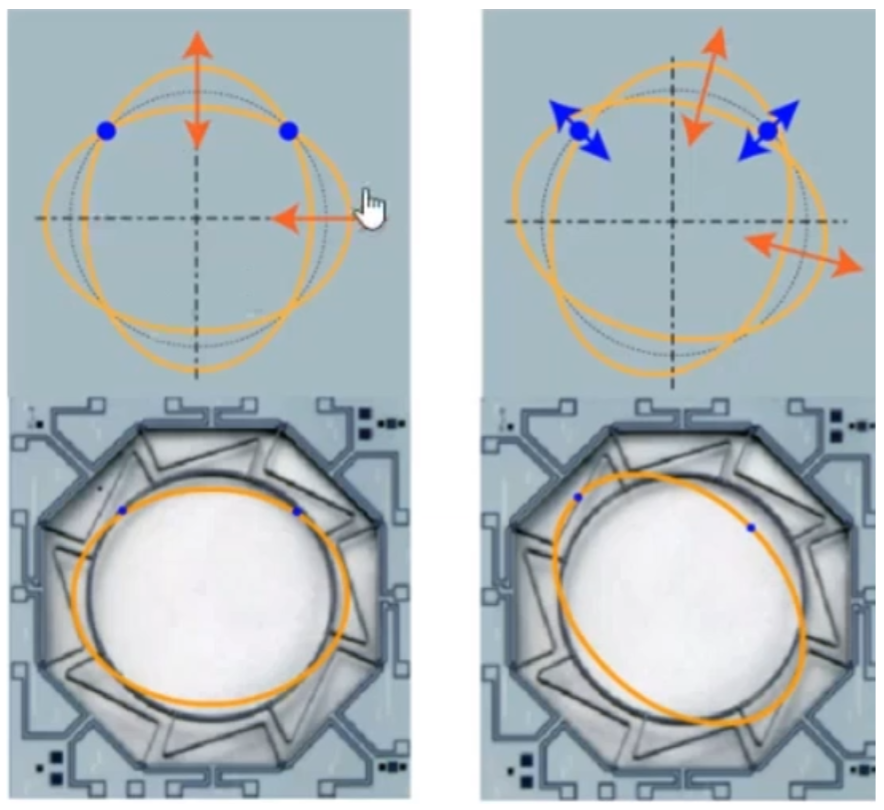
\includegraphics[scale = 0.40]{img/VibrujiciPrstenec.png}
\end{figure}

\subsubsection*{Optické gyroskopy- Sagnacův jev}
\begin{itemize}
    \item Měří se rozdíl dvou světelných svazků vyslaných proti směru a ve směru otáčení.
    \item Sagnacův jev - zvýšení (snížení) rychlosti o hodnotu v = w * r
    \item Ve stejný čas pošlem paprsek oběma směry a zpátky ve stejný čas - Když dráhu roztočíme, tak signál, který jsme poslali do protisměru dorazí dřív, vzniká tak rozdíl fáze, který měříme.
    \item Funguje nezávisle na indexu lomu
\end{itemize}

\begin{figure}[h]
    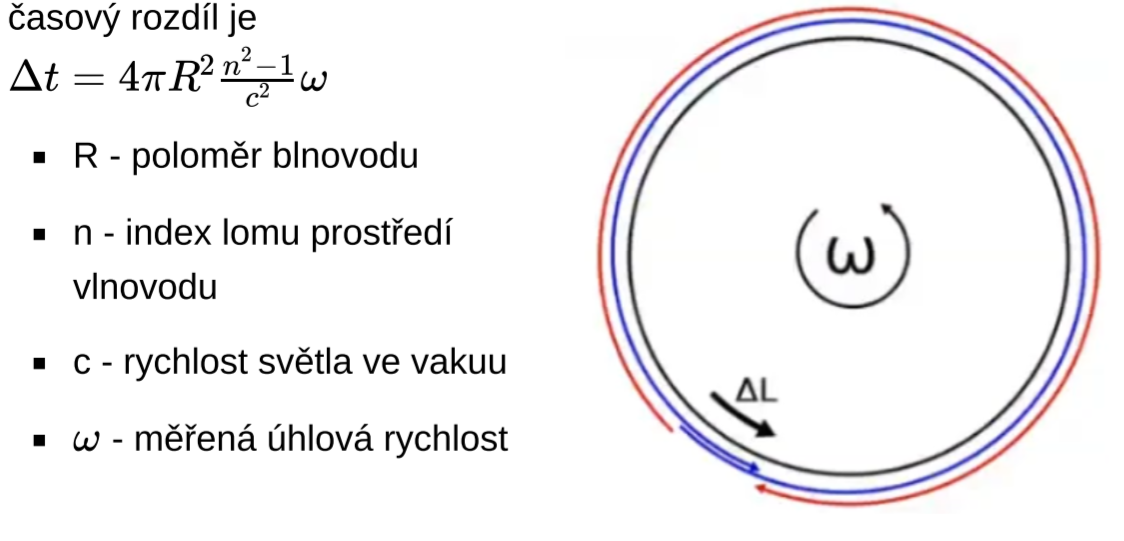
\includegraphics[scale = 0.40]{img/sagnac.png}
\end{figure}

\subsubsection*{Optické gyroskopy - FOG}
\begin{itemize}
    \item Optické vlákno, které je měřící element. Ze zdroje záření se pošle paprsek, ten se na polopropustném zrcátku rozdělí na měřící a referenční svazek. Měřící se pak ještě rozdělí na další dva svazky a to kvůli tomu, aby šly do optického vlákna každý jiným směrem.
    \item Na fázovém (de)modulátoru (FM) sledujeme vzniklé interferenční jevy.
    \item Kdybychom vyhodnocovali fázový rozdíl při nulové úhlové rychlosti, tak bude nulový, protože na vrcholu sinusovky je víceméně nulová citlivost a fázový rozdíl se tam blbě měří.
\end{itemize}

\begin{figure}[h]
    \centering
    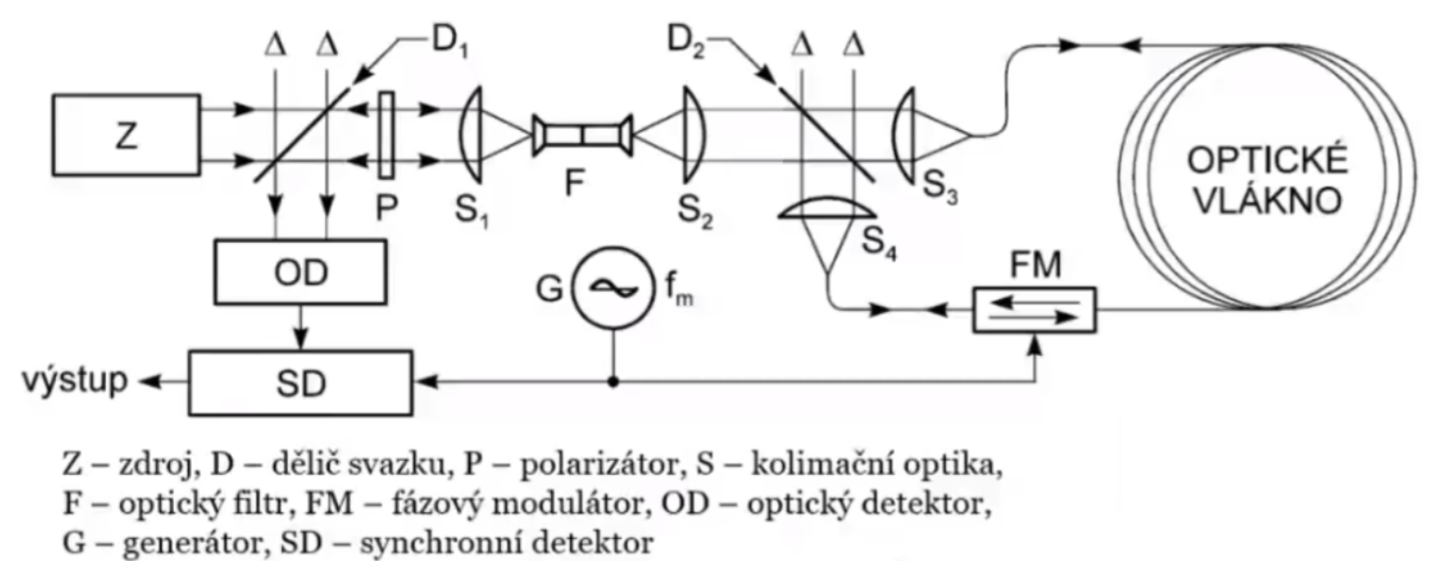
\includegraphics[scale = 0.40]{img/fog.png}
\end{figure}

\subsubsection*{Optické gyroskopy - RLG}
\begin{itemize}
    \item Zásadní rozdíl je v tom, že dutina rezonátoru je snímač, který vyhodnocuje rychlost.
    \item Rozměr rezonanční dutiny nám ovlivňuje výstupní vlnovou délku
    \item V dutině jsou současně dva rezonátory (pro oba směry), když se dutina neotáčí a dráha je stejná.
    \item Pokud budeme otáčet, tak dráha pro jeden foton bude kratší.
    \item Na detektoru se nám potkávají lasery s rozdílem kmitočtu, čím větší je úhlová rychlost, tím větší je rozdíl kmitočtů mezi lasery
\end{itemize}

\begin{figure}[h]
    \centering
    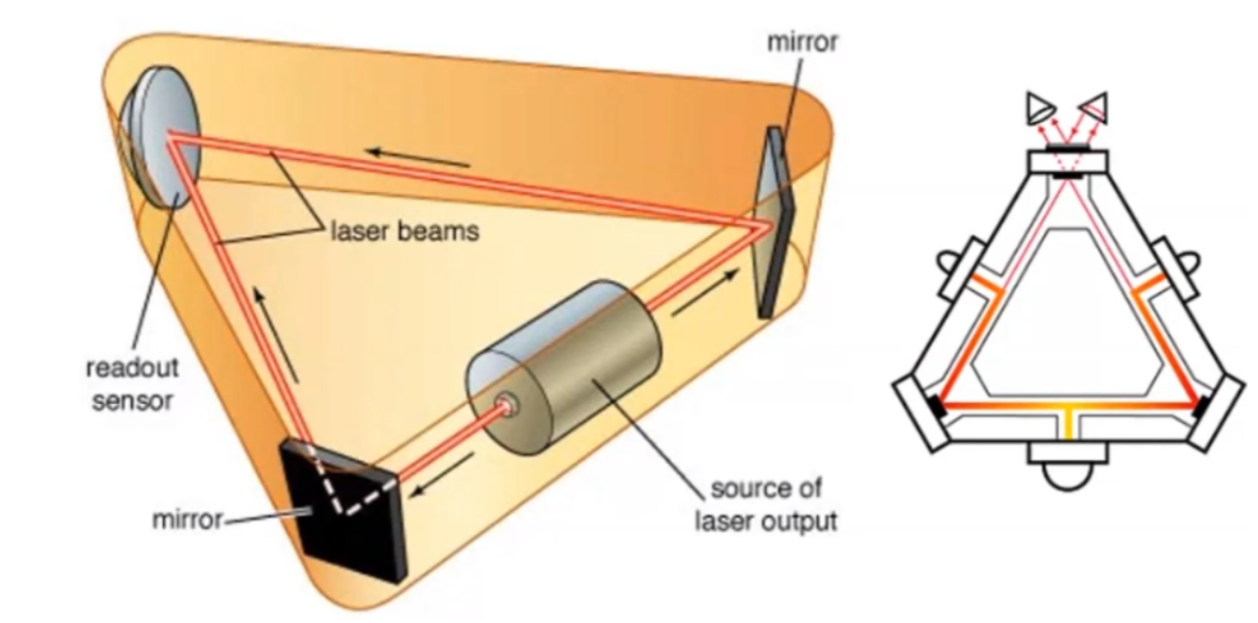
\includegraphics[scale = 0.40]{img/lgr.png}
\end{figure}

\subsubsection*{Srovnání gyroskopů}
\begin{figure}[h]
    \centering
    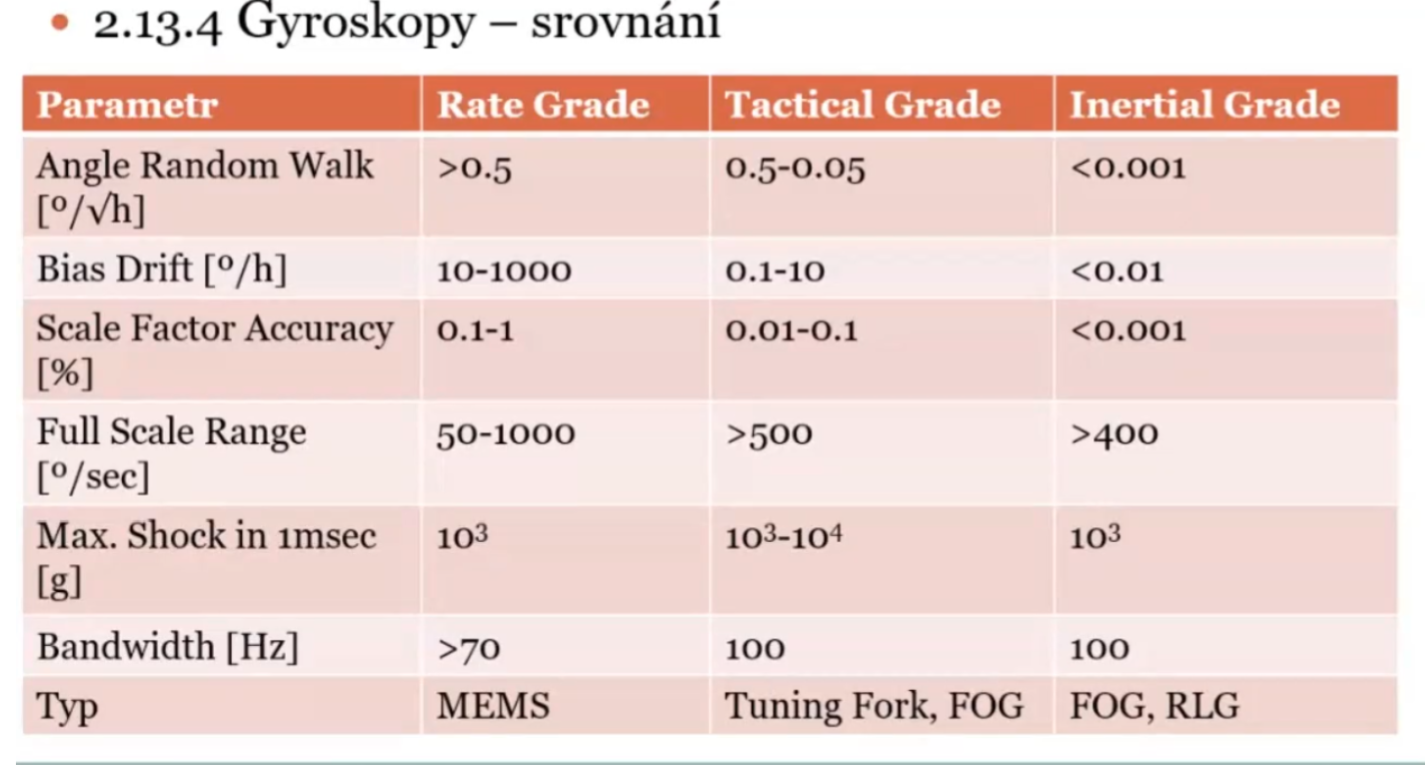
\includegraphics[scale = 0.40]{img/srovnaini.png}
\end{figure}

\section{Tenzometry, snímače síly, hmotnosti, momentu a tlaku }


\section{Měření průtoku, základní principy objemových, rychlostních a hmotnostních průtokoměrů}
\subsection*{Základní pojmy}
\begin{itemize}
    \item Problém s tím, že měřené médium je pokaždé jiné a hodí se tím pádem jiný snímač.
    \item Urostřed toku největší rychlost - tření od stěn se postupně snižuje
    \item Reynoldsovo číslo - Souvislost setrvačné síly a viskozity = čím vyšší číso, tím nižší odporové síly. Když toto číslo přesáhne 3000, průtok přejde na turbulentní propudění - zvyšuje se jeho hydraulický odpor, proudy se pohybují chaoticky, porušený rychlostní profil.
\end{itemize}
\begin{figure}[!h]
    \centering
    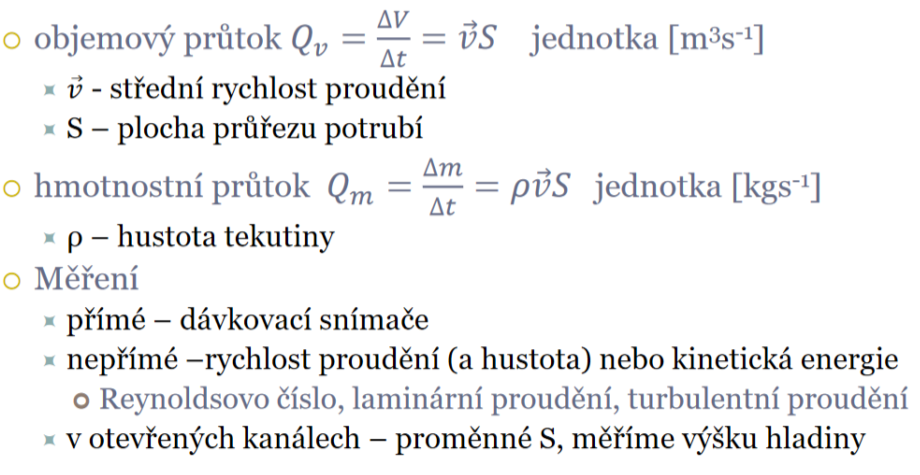
\includegraphics[scale = 0.8]{img/prutokZaklad.png}
\end{figure}

\begin{figure}[!h]
    \centering
    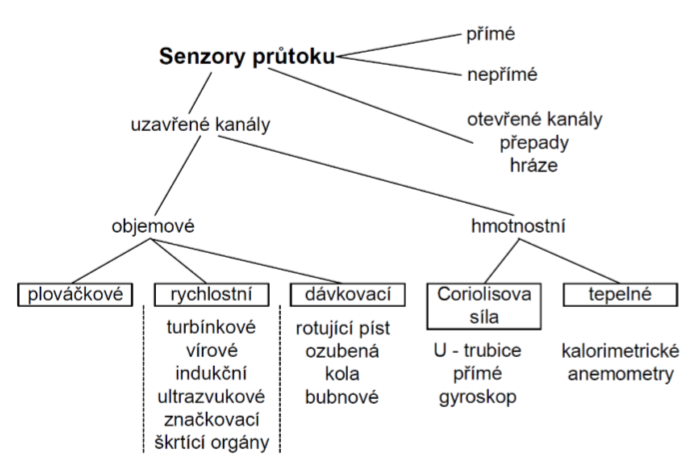
\includegraphics[scale = 1]{img/proudoverozdeleni.png}
\end{figure}

\subsection*{Plováčkové průtokoměry}

\subsubsection*{Rotametry - průtokoměry s proměnným průřezem}
\begin{itemize}
    \item Kuželovitý plovák jako indikátor rovnováhy sil
    \item Tekutina proudící zespodu plovák nadnáší, ten má drážky po obvodu pro stabilizaci rotace.
    \item Vztlaková síla díky kuželovitému tvaru umožňuje tlakovou diferenci.
    \item V určitém místě se síly vyrovnají. Tato hodnota se poté odečte na stupnici. 
    \item Snímá se bezkonaktně poloha.
    \item Opakovatelnost 0.25 \%, malá tlak. ztráta
\end{itemize}

\begin{figure}[h]
    \centering
    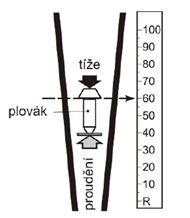
\includegraphics[scale = 1]{img/rotatometr.png}
\end{figure}

\subsubsection*{Turbínkové a lopatkové snímače průtoku}
\begin{itemize}
    \item Protékající tekutina roztočé vrtulku, měří se bezkontaktně Otáčky
    \item Citlivost cca 3 \% z rozsahu, přesnost až 0.1 \%, poměrně velká chyba při malých průtocích
    \item Lopatkové - lopatky kolmo na tok, levnější než turbínkové
    \item Turbínkové - lopatky souběžně na tok
\end{itemize}

\begin{figure}[h]
    \centering
    \includegraphics[scale = 0.7]{img/lopatkaaturbin.png}
\end{figure}

\section*{Vírové snímače průtoku}
\begin{itemize}
    \item Do průtoku vložíme překážku
    \item Za překážkou se tvoří víry, překročí se reynoldsovo číslo, víry se začnou nastřídačku odtrhávat - tzv- Karmánová stezka, kmitoče vírů je přímo úměrný rychlosti průtoku
    \item Víry jsou detekovány: \begin{itemize}
        \item Ze změn rychlosti proudění - tepelný anemometr, ultrazvuk
        \item Ze změn tlaku - tenzometry, kapacitně, piezoelektricky
    \end{itemize}
    \item Jsou víry - měříme, nejsou- neměříme
    \item Problém s vyhodnocením vírů
\end{itemize}

\begin{figure}[h]
    \centering
    \includegraphics[scale = 1]{img/ViroveSnimaceTrojskyVirPhishingBackdoormrkmrk.png}
\end{figure}

\subsection*{Ultrazvukové snímače průtoku}
\begin{itemize}
    \item Princip je skládání rychlosti ultrazvukového signálu a proudícího média
    \item Rychlost je úměrná rozdílu doby průletu ultrazvukového signálu ve směru (delta t1) a v protisměru (delta t2) proudící tekutiny.
    \item Princip je takový, že máme proti sobě umístěné dva piezoelektrické měniče, které mohou fungovat jako vysílače a přijímače \begin{itemize}
        \item Z jedné strany se pošle ultrazvukový signál, ten letí na druhou stranu k přijímači a měří se čas. Pak se pošle zpátky a opět se měří čas.
        \item Když se médium nehýbe, tak čas tam a zpět je stejný.
        \item Když se médium hýbe, tak k rychlosti šíření signálu se přicítá relativní rychlost pohybujícího se média. Takže v jednom směru je signál zrychlován a ve druhém zpomalován. Počítá se rozdíl času
        \item Jejich diferenční zapojení maže okolní vlivy.
        \item Výhoda je dodatečná montáž na potrubí, tím, že se montuje jen z "venku", tak v potrubí nic nepřekáží = nejmenší tlaková ztráta.
        \item Jsou poměrně drahé a toto řešení není tak triviální jak se zdá.
    \end{itemize} 
\end{itemize}

\subsection*{Indukční snímač průtoku}
\begin{itemize}
    \item Pro vodivé kapaliny (i voda), pohyb "vodiče" v magnetickém poli generuje napětí U = Blv
    \item Pro zpracování lepší střídavé mag. pole
    \item Levný, větší rozsah měřených průtokoměrů
    \item Princip podobný jako dynamo - pohybuje se vodič v magnetickém poli, na jeho koncích naměříme napětí.
    \item Interakce mag. pole s kapaliny s vnějším - lorentzova síla.
    \item Na stěnách trubky se začnou hromadit kladné ionty a na druhé záporné. Tím se dostane rozdíl potenciálu.
    \item Výsledkem je střídavé magnetické pole => homogenní magnetické pole a měří se rozdíl napětí na bočních elektrodách, které je přímouměrné magnetické indukci.
    \item 
\end{itemize}

\begin{figure}[h]
    \centering
    \includegraphics[scale = 1]{img/indukceViiir.png}
\end{figure}

\subsection*{Snímače průtoku s tlakovou diferencí}
\begin{itemize}
    \item Založen na měření tlakového spádu na zúženém místě potrubí
    \item Čkrtící orgán - clona, dýza, Venturiho trubice, Pitotova trubice
    \item Rozdíl tlaku se měří diferenčním snímačem tlaku
    \item Typicky průtokoměr pro měření páry
    \item Nelineární závislost
    \item Není třeba nic normalizovat - vše je spočítané
    \item Kritický parametr - snaha mít, co nejmenší tlakové ztráty a největší differenci
    \item Potřebujeme velký kus potrubí
\end{itemize}

\subsection*{Dávkové snímače průtoku}
\begin{itemize}
    \item Plní se nějaký objem průtoke, jakmile se naplní, tak se vylije a plní se znova.
    \item Existují různé varianty - rotační, pístové, membránové
    \item Pohyb je způsoben rozdílem sil nebo točivých momentů vyvolaných vstupním a výstupním tlakem
    \item Používá se pro plyny a kapaliny v rozsahu l/h, m3/h
\end{itemize}

\begin{figure}[h]
    \centering
    \includegraphics[scale = 1]{img/davkovaci.png}
\end{figure}
\newpage
\begin{itemize}
    \item Princip zubového čerpadle - médium tlačí na písty, které se kvůli tomu točí a definovaný průtok se tak dostane na druhou stranu
    \item Přesné měření průtoku oleje - kalibrační, referenční
    \item Musí být dobře těsněné, čisté a samomazné
\end{itemize}

\subsection*{Hmotnostní snímač průtoku}
\begin{itemize}
    \item Princip založen na detekci silového působení hmotného pohybujícího elementu tekutiny
    \item Praktické provedení - U trubice, Delta trubice, přímá trubice
    \item Trubice je rozkmitána silou FM na rezonančním kmitočtu, FC způsobí zkroucení, snímači polohy se vyhodnocuje fázový posun
    \item Přesnost až 0.1 \%, nezávislost na viskozitě, tlaku, teplotě.
\end{itemize}

\begin{figure}[h]
    \centering
    \includegraphics[scale = 1]{img/FC.png}
\end{figure}

\begin{figure}[h]
    \centering
    \includegraphics[scale = 1]{img/hmotnostniprutok.png}
\end{figure}

\begin{itemize}
    \item Využívá se Coriolisovy síly - hmotný bod se nám bude pohybovat určitou rychlostí a současně bude v nějakém otáčejícím/kmitajícím systému \begin{itemize}
        \item Otáčející se bod - element kapaliny - trubka, kterou nuceně rozmitáme - kapalina uvedena do rotačního pohybu - elektromagneticky rozkmitáváme
        \item Když se kapalina v trubce pohybuje, tak začne působit Coriolisova síla, na jedné straně působí dolů, na druhé nahoru.
        \item Měřená veličina je amplituda zkroucení na obou maximech - snímače polohy -> pokud tam něco poteče, bude fázový posun, pokud nepoteče, stejná fáze.
        \item Je zde problém s bublinkama - mění se tím skokově hustota - blbě se drží snímač v rezonanci
    \end{itemize}
    \item Technicky velmi náročné mechanický systém vyrobit a ten fázový rozdíl bývá ve vtečinách - "fes malo"
    \item Drahé, využívá se u drahých paliv, čerpací stanice.
    \item Z rezonančního kmitočtu můžem měřit i hustotu
    \item Vadí mu skokové změny, teplotní, znečištění a celkově prostředí mu nevadí.
\end{itemize}

\subsection*{Tepelné hmotnostní snímače průtoku}
\begin{itemize}
    \item Zahříváme nějaký element a měříme odvod tepla prouděním - proudící plyn/kapalina
    \item Odvod tepla souvisí s hustotou tekutiny - čím hustší, tím větší přestup tepla
    \item Měříme ochlazení drátku - termoanemometrie \begin{itemize}
        \item Udržuje konstantní proud nebo konstantní teplotu
        \item Okolí mu odebírá teplo
        \item Měří se kolik proudu musíme do obvodu pouštět, aby měl drát stejnou teplotu
    \end{itemize}
    \item Měříme přenos tepla - kalorimetrický princip \begin{itemize}
        \item Měříme rozložení teploty v okolí zdroje
        \item Protékající plyn deformuje teplotní pole
        \item Komplikované při větších průtocích - dělá se odbočka na menší průřez
        \item Provovnání pomocí můstku
    \end{itemize}
    \item Využívají se ve vzduchotechnice, průtok benzínu
\end{itemize}

\begin{figure}[h]
    \centering
    \includegraphics[scale = 1]{img/kalorime.png}
\end{figure}

\subsection*{Snímače průtoku v otevřených kanálech}
\begin{itemize}
    \item Princip založen na měření výšky hladiny v průtokovém kanále definovaného typu - přeliv, žlab
    \item Snímač výšky hladiny obvykle ultrazvukový
    \item Snímače výšky hladiny - nespojité (plovákové, vibrační, ultrazvuk,...), spojité (diferenčí tlak, meření vztlakové síly, kapacitní,...)
\end{itemize}

\subsection*{Srovnání}

\begin{figure}[h]
    \centering
    \includegraphics[scale = 1]{img/srovnaniprutok.png}
\end{figure}

\section{Kontaktní snímače teploty (dilatační, odporové, termoelektrické)}


\section{Měření záření (tepelné a kvantové snímače IR záření, snímače ionizujícího záření)}


\section{Chemické snímače}
Slouží pro měření koncentrace výskytu látek v některých výrobních, provozních, skladovacích, měřících a dalších procesech.\\
Chemický senzor je zařízení, které snímá sledovanou chemickou veličinu a definovaným způsobem ji transformuje chemicko-fyzikálním převodem (receptor + převodník) na veličinu výstupní.\\
Základní pojmy:
\begin{itemize}
    \item Adsorpce - materiál na svém povrchu naváže kontakt s prostředím
    \item Absorpce - látka vnikne do objemu
    \item Látková koncentrace - měření kolik objemu nějaké látky je v celkovém objemu
          \begin{itemize}
              \item Molový poměr
              \item Hmotnostní - hmotnost jedné látky v celém objemu
              \item Objemová míra - ppm(parts per million), ppb(parts per billion)
          \end{itemize}
    \item Selektivita - jestli je snímač schopen stanovit koncentraci nějaké konkrétní látky ve směsi. Čím vyšší selektivita tím větší univerzálnost a tím větší cena.
    \item Oxidačně-redukční potenciál - jak ochotně prostředí odevzdává kyslík
\end{itemize}
Často se měří koncentrace vodíkových iontů \(pH = -\log(fc_{H+}) = -\log(a_{H+})\)\\

\subsection{Fyzikální principy}
\subsubsection{Rezonanční piezoelektrické snímače}
\subsubsection*{SAW - Surface Acoustic Wave}
Máme pár dvouelektrodových systémů na destičce z piezoelektrického materiálu. Jeden elektrodový pár slouží jako generátor vibrací a druhý jako jejich snímač.\\
Když na elektrody na generátoru vybrací přivedeme napětí, které je naladěné na rezonační kmitočet piezoelektrické vrstvy, tak vybudíme povrchovou vlnu, který cestuje skrze zkoumaný materiál. Během cesty přes materiál se vlna tlumí, kvůli viskozitě materiálu. Jakmile tato vlna narazí do piezoelektrické vrstvy snímače, vlna materiál deformuje a to na elektrodách vytvoří náboj.\\
Měříme potom diferenci kmitočtů mezi vlnou vyslanou a vlnou přijatou. Z toho poznáme jak se mění hmotnost objemu.\\
\begin{figure}[h!]
    \centering
    \includegraphics[scale = 0.1]{img/ChemPiezoEl.png}
\end{figure}

\subsubsection{Tepelně vodivostní snímače}
Analýza binárních směsí, kde měříme odvod tepla po okolí.\\
Využíváme změny tepelné vodivosti, lze využít pouze u dvou materiálů, které mají významně rozdílnou tepelnou vodivost.\\
Měříme odvod tepla do okolí a pokud převažuje látka s lepší tepelnou vodivostí, tak odvod tepla do okolí je větší a když ne, tak menší.\\

\subsubsection{Paramagnetické snímače kyslíku}
Využívá se paramagnetických vlastností kyslíku(mírně zesilují vnější magnetické pole).\\
Dva principy: magnetomechanický a termomagnetický.\\
\subsubsection*{Magnetomechanický}
Je založen na přítomnosti tělíska z diamagnetického materiálu v nehomogenním magnetickém poli. Diamagnetické materiály jsou takové, které zeslabují magnetické pole a jsou jím odpuzovány.\\
V magnetickém poli senzoru jsou vloženy 2 koule spojené tyčinkou, tak že tvoří tvar činky, které jsou z diamagnetického matierálu. Po přivedení molekul kyslíku do senzoru se začne činka odkloňovat z magnetického pole určitou silou.\\
Na čince je umístěno zrcátko na které je směřován paprsek z LED diody, z něj je odražen na 2 fotodiody. Síla, kterou je činka vytlačována z pole je tak převedena na elektrický signál. Aby činka neodrotovala z magnetického pole je nutno ji udržovat na místě pomocí elektrického proudu. Tento proud je generován z fotodiod a je přímo úměrný obsahu kyslíku.\\
\begin{figure}[h!]
    \centering
    \includegraphics[scale = 0.5]{img/Paramag1.png}
\end{figure}

\subsubsection*{Termomagnetický}
V komoře snímače je umístěno topné těleso, které ohřívá kyslí přítomý v této komoře. Jakmile se kyslík ohřeje nad Curieovu teplotu, ztrácí své paramagnetické vlastnosti a je z komory vytlačen studeným kyslíkem, tímto vzniká proudění, které měříme anemometrem. Čím větší proudění je, tím větší je koncentrace kyslíku.\\

\subsubsection{Vodivostní snímače}
Konduktometrie je využívání elektrolytické(iontové) elektrické vodivosti roztoků k měření.\\
Pro měření kapalin.\\
Nízká selektivita.\\
Princip: na elektrody připojíme vnější elektrické pole, roztokem začne procházet proud a měříme mezi elektrodami.\\
Elektrody můžeme napájet jak stejnosměrně tak střídavě, avšak u stejnosměrného měření je problém takzvaná polarizace elektrod. Ta je založen na tom, že iont se fyzicky nemůže do elektrody dostat a tak zůstává na povrchu a tím vytvoří dvouvrstvu náboje, která se pak tváří jako elektrický bipól a odpuzuje další přicházející ionty a od určitého počtu iontů přestane proud procházet mezi elektrodami, proto měříme střídavě.\\
\newpage
\begin{figure}[h!]
    \centering
    \includegraphics[scale = 0.1]{img/ElektrodSonda.png}
\end{figure}
Na obrázku schéma planárních elektrod a jejich elektrické pole.\\
\begin{figure}[h!]
    \centering
    \includegraphics[scale = 0.1]{img/NahrSchemaVodiv.png}
\end{figure}
Kmitočet se volí kolem desíti kHz.\\
\subsubsection*{Čtyřelektrodový snímač}
Využije se toho, že máme snímací elektrody(2,3), kterými neprochází proud, čímž se výrazně potlačí polarizační jevy, se kterýma byl v předchozím případě problém.\\
Oddělené napěťové a proudové elektrody.\\
\begin{figure}[h!]
    \centering
    \includegraphics[scale = 0.05]{img/CtyrElektr.png}
\end{figure}

\subsubsection*{Bezkontaktní snímač konduktivity}
Zcela potlačuje efekt polarizačních jevů.\\
Funguje to tak, že máme trubičku ve tvaru uzavřeného kruhu, kde prochází kapalina a na ní jsou dva magnetické obvody(primární a sekundární).\\
Primární vybudí magnetický tok a kapalina nám vytváří jeden závit(n2) a má nějakou impedanci(Rx), který podle ohmova zákona určuje, kolik tam teče proudu a pak u druhého proudového transformátoru se proud převede a měří.\\
\begin{figure}[h!]
    \centering
    \includegraphics[scale = 0.1]{img/BezkSnimVod.png}
\end{figure}

\subsubsection{Iontové spektrometry}
\subsubsection*{Hmotnostní spektrometry}
Hmotnostní spektrometry, které jsou založeny na měření dráhy iontu v magnetickém poli. Hmotnost iontu má vliv na zakřivení této dráhy.\\
Princip: Vezmeme vzorek látky a zionizujeme ji(elektrickým výbojem nebo ionizujícím zářením). Ionty pošleme do po určité dráze do magnetického pole. Iont jako nabitá částice, která si vytváří své vlastní magnetické pole interaguje s vnějším magnetickým polem a dochází ke změně dráhy(Lorentzova síla působí kolmo na vektor MP a vektor rychlosti). To zakřivení bude různé podle toho, jaký je náboj iontu(chemické složení) a jakou má hmotnost a podle toho dopadne na určité místo matice detektorů(PN přechody, nebo fotoelektrický jev) a podle množství kolik náboje vygenerujeme a kam dopadne, tak z toho můžeme usuzovat, jaké bylo původní složení zkoumané látky.\\
\subsubsection*{Měření pohyblivosti iontů}
Opět musíme zionizovat prostředí a částice jsou urychleny napěťovým impulsem.\\
Jen jeden detektor a měří se, za jak dlouho tam doletí a jaká je hodnota náboje.\\
Čím větší náboj, tím větší impuls jí dáme a čím větší hmotnost tím pomalejší.\\
Ionty jsou v el. poli impulsně urychleny, měří se tvar a zpoždění proudového impulsu na sběrné elektrodě.\\
Využití pro detektory organických látek, bojových plynů, výbušnin.\\

\subsection{Chemické principy}
Dělí se na potenciometrické a amperometrické. Jestli elektrodama prochází nebo neprochází proud. Jestli se mění napětí na elektrodovém systému v závislosti na koncentraci.\\
\subsubsection{Polovodičové snímače plynů}
Oxidační princip
\begin{itemize}
    \item Detekce oxidačních nebo redukčních plynů
    \item Díky oxidaci povrchové vrstvy vznikají volné elektrony a navenek se to projeví jako změna vodivosti
    \item Detekce plynů sporáků.\\
\end{itemize}
Snímače s povrchovou detekcí:
\begin{itemize}
    \item Princip založen na změně vodivosti povrchové vrstvy kysličníku adsorpcí testovaného plynu
    \item Redukční plyny vodivost zvyšují, oxidanční snižují
    \item Pracovní teplota kysličníkové vrsty je 200 až 450°C
\end{itemize}
\begin{figure}[h!]
    \centering
    \includegraphics[scale = 0.1]{img/PovrchDetek.png}
\end{figure}
Snímače s objemovou detekcí:
\begin{itemize}
    \item Princip založen na změně vodivosti vnitřní struktury kysličníku absorpcí testovaného plynu.
    \item Citlivou kysličníkovou vrstvu musíme zahřát na poměrně vysokou teplotu a díky absorpovanému kyslíku dochází ke změně vodivosti, vyhodnocujeme změnu vodivosti vrstvy.
    \item Kyslík propojuje oxidy mezi sebou a dochází ke zvětšení vodivosti.
    \item Pracovní teplota kysličníkové vrstvy je až 900°C
\end{itemize}

\subsubsection{CHEMFET snímače}
Adsoprcí měřeného plynu vznikne dipólová vrstva generující napětí na řídící elektrodě MOS tranzistoru a tím ovlivňuje vodivost kanálu.\\
Na řídící elektrodě je chemická vrstva, která na měřený plyn/kapalinu zaregauje a vytvoří polarizační vrstvu(chemickou vrstvou povrch zpolarizuje), tím se vytvoří volný náboj, který na kapacitě přechodu(gate) se chová jako napětí a to ovlivňuje indukovaný kanál.\\
\begin{figure}[h!]
    \centering
    \includegraphics[scale = 0.2]{img/CHEMFET.png}
\end{figure}

\subsubsection{Termokatalytické snímače - Pelistory}
Principem je měření tepla vzniklého pry katalytickém spalování hořlavých a výbušných látek.\\
Katalytická reakce je taková kde máme chemickou látku, která je nutná k tomu aby proběhla chemická reakce, ale sama se tou reakcí nespotřebuje.\\
Jako katalyzátory se používají kovy na bázi platiny.\\
Princip: Máme vyhřívaný platinový drátek, který je ohříván. Jakmile do struktury snímače pronikne přes vnější porózní materiál hořlavý či výbušný plyn, tak dojde ke spálení. Navenek se to projeví tak, že se uvolňuje teplo, díky tomu se zahřeje platinový drátek, který slouží jako topné těleso a senzor zároveň.\\
Čím větší je koncentrace plynu, který je možno spálit tím menší proud musíme do drátku dodat abychom reakci zahájili.\\
\begin{figure}[h!]
    \centering
    \includegraphics[scale = 0.2]{img/Pelistor.png}
\end{figure}

\subsubsection{Elektrochemické snímače}
Využíváme chemické reakce na kovové elektrodě v elektrolytu.\\
Pokud strčíme jakýkoliv kov do kapaliny, dojde k chemické reakci na jeho povrchu. Tím se stane elektroda buď kladnější nebo zápornější(přidáním či odebráním elektronů). Ponořením vznikne potenciál, ale potřebujeme ještě druhý referenční potenciál, tudíž potřebujeme v elektrolytu 2 kovy. Pak můžeme měřit rozdíl potenciálů. Poté rozlišujeme jestli elektrodami protéká proud(amperometrie) či neprotéká proud(potenciometrie).\\
Elektrochemické reakce na kovové elektrodě:
\begin{itemize}
    \item Anodická oxidace - přijímání elektronů
    \item Katodická redukce - odevzdávání elektronů
\end{itemize}
Typ reakce je ovlivněn materiálem elektrody, složením elektrolytu a elektrodovým potenciálem.\\
Způsob vyhodnocení potenicálu:
\begin{itemize}
    \item Potenciometrie - bezproudé měření napětí mez měřící a referenční elektrodou, například měření pH
    \item amperometrie
          \begin{itemize}
              \item Záleží z jakého materiálu elektrody jsou, protože některé jsou schopny neustále obnovovat polarizační vrstvu a některé ne. To se projeví tím, že při konkrétní hodnotě proudu se efekt polarizace přestane projevovat a změní se napětí na elektrodách
              \item Měříme proud pro různé hodnoty napětí stejnosměrného přepětí a tím dokážem změřit koncentraci volných iontů v kapalině, protože v určitém okamžiku ionty přestanou být schopny dodávat odebraný náboj z elektrod
              \item Koncentraci pak stanovíme rozdílem napětí mezi elektrodami. Když budeme na polarizované elektrodě náboj odebírat, tak se bude napětí měnit v závilosti na koncentraci iontů. Na nepolarizované tato závislost není a díky tomu máme referenční měřidlo.
          \end{itemize}
\end{itemize}
\subsubsection*{Elektrochemické potenciometrické snímače}
Potenciometrické měření pH
\begin{itemize}
    \item Měření kyselosti a zásaditosti roztoků
    \item Měřící elektroda z (porézního skla) propustná pro ionty
    \item Referenční elektroda kalomelová s konstantním potenciálem
    \item Vyhodnocujem napětí na výstupních elektrodách, rozdíl odpovídá koncentraci vodíkových iontů
    \item Problémem je bezproudé měřením to znamená, že výstupní impedance snímače extrémně vysoká a vstupní odpor voltmetru musí být minimálně o dva větší řády větší
    \item Závislé na teplotě
    \item Dobrá citlivost
\end{itemize}
\begin{figure}[h!]
    \centering
    \includegraphics[scale = 0.1]{img/PotencPH.png}
\end{figure}

Iontově selektivní metody, ISFET:
\begin{itemize}
    \item kromě univerzálních skleněných elektrod existují i elektrody citlivé pouze na některé ionty, díky iontově selektivní membráně a vhodnému elektrolytu
\end{itemize}
\begin{figure}[h!]
    \centering
    \includegraphics[scale = 0.1]{img/IontSelMet.png}
\end{figure}
Potenciometrie s tuhým elektrolytem
\begin{itemize}
    \item pro měření kyslíku - např. lambda sondy
    \item Výstupní napětí odpovídá rozdílu parciálních tlaků kyslíku
    \item Potenciál daný množstvím kyslíku
\end{itemize}
\begin{figure}[h!]
    \centering
    \includegraphics[scale = 0.2]{img/TuhElekt.png}
\end{figure}

\subsubsection*{Elektrochemické amperometrické snímače}
Chemickou reakcí se vytvoří vrstva, kdy se změnou napětí mění procházející proud.\\
\begin{figure}[h!]
    \centering
    \includegraphics[scale = 0.2]{img/Amperomet.png}
\end{figure}

\subsection{Optické a optoelektronické principy}
Využívá se obsorpce elektromagnetického záření v měřeném prostředí dle Lamber-Beerova zákona.\\
Zdroj záření - výbojky, žárovky, laserové diody.\\
Detektor - bolometry, pyroelektrické články, fotoodpory, fotodiody, tepelně-pneumatické detektory.\\
máme zdroj světla, prochází pipetou s detekovaným plynem a my měříme útlum v jednotlivých pásech.\\
\begin{figure}[h!]
    \centering
    \includegraphics[scale = 0.2]{img/OptPrinc.png}
\end{figure}

\subsection{Biosnímače}
Předsazená vrstva, která je biocitlivá a výsledkem je změna koncentrace již měřitelné látky - kyslík, pH, apod.\\
Transformují biologicky sledovanou látku na látku, kterou umíme měřit.\\
\begin{figure}[h!]
    \centering
    \includegraphics[scale = 0.1]{img/Biosnimace.png}
\end{figure}

\subsection{Snímače vlhkosti}
Absolutní:
\begin{itemize}
    \item Absolutní vlhkost, směšovací poměr
    \item Typicky koncentrace vodních par ve vzduchu
\end{itemize}
Relativní:
\begin{itemize}
    \item Relatnivní vlhkost, rosný bod
    \item Závislost na teplotě
\end{itemize}
\subsubsection{Sorpční snímače vlhkosti}
Pára mění vodivost nebo kapacitu.\\
Princip založen na změně fyzikálně-chemických vlastností materiálu detektoru vlivem vlhkosti.\\
Vlasové vlhkoměry, odporové nebo kapacitní vlhkoměry.\\

\subsubsection{Psychometr}
Snímač relativní vlhkosti, princip založen na měření rozdílu teploty vlhčeného a suchého snímače, vlhký snímač je ochlazován výparným teplem.

\subsubsection{Snímač rosného bodu}
Detekujeme orosení zrcátka přerušením optické vazby.\\
Máme zdroj světla dopadající na zrcátko, které je ochlazováno peltierovým článkem a měříme teplotu, při které dojde k zamrznutí vody, to zjistíme tak, že se na zrcátku přestane odrážet signál. Teplotě zamrznutí odpovídá rosný bod, pomocí kterého lze dopočítat relativní či absolutní vlhkost.\\
\begin{figure}[h!]
    \centering
    \includegraphics[scale = 0.1]{img/RosBod.png}
\end{figure}